\documentclass[11pt]{book}  % 11 point font size is recommended

% Non-CVSSP members only: If you want to make your thesis fatter, you can
% print single-sided by adding "oneside" to the documentclass options:
%\documentclass[oneside,11pt]{book} 

\usepackage{a4,graphicx,eimthesis} 
\usepackage[usenames,dvipsnames]{color}
\usepackage{acronym}
\usepackage[table]{xcolor} %Table colours for highlights
\usepackage[cmex10]{amsmath}
\usepackage{amsfonts}
\usepackage{listings}
\usepackage{algorithm}
\usepackage{nomencl}
\usepackage{quotchap}
\usepackage[toc]{appendix}
\usepackage{wasysym} %For male and female symbols
%\usepackage{draftwatermark}

%\SetWatermarkText{DRAFT}
%\SetWatermarkLightness{0.9}
%\SetWatermarkScale{4}

\acrodef{NVC}{Non-Verbal Communication}
\acrodef{FACS}{Facial Action Coding System}
\acrodef{SVR}{Support Vector Regression}
\acrodef{SVM}{Support Vector Machine}
\acrodef{RBF}{Radial Basis Function}
\acrodef{AU}{Action Unit}
\acrodef{IP}{Internet Protocol}
\acrodef{UK}{United Kingdom}
\acrodef{GBR}{Great Britain}
\acrodef{US}{United States}
\acrodef{SVM}{Support Vector Machine}
\acrodef{ICA}{Independent Component Analysis}
\acrodef{LMA}{Levenberg--Marquardt Algorithm}
\acrodef{LBP}{Local Binary Pattern}
\acrodef{PCA}{Principal Component Analysis}
\acrodef{CKD}{Cohn-Kanade AU Coded Facial Expression Database}
\acrodef{HMM}{Hidden Markov Model}
\acrodef{ROC}{Receiver Operating Characteristic}
\acrodef{MIL}{Multiple Instance Learning}
\acrodef{URL}{Uniform Resource Locator}
\acrodef{LP}{Linear Predictor}
\acrodef{ASM}{Active Shape Model}
\acrodef{AAM}{Active Appearance Model}
\acrodef{HCRF}{Hidden Conditional Random Field}
\acrodef{iHCRF}{Infinite Hidden Conditional Random Field}
\acrodef{CORF}{Conditional Ordinal Random Field}
\acrodef{NMF}{Non-negative Matrix Factorisation}
\acrodef{MNN}{Modified Nearest Neighbour}
\acrodef{LLR}{Logistical Linear Regression}
\acrodef{CRF}{Conditional Random Field}
\acrodef{NMF}{Non-negative Matrix Factorization}
\acrodef{DCT}{Discrete Cosine Transform}
\acrodef{LPQ}{Local Phase Quantization}
\acrodef{FLD}{Fisher Linear Discriminant}
\acrodef{SVDD}{Support Vector Data Description}
\acrodef{EM}{Expectation Maximization}
\acrodef{kNN}{k-Nearest Neighbour}
\acrodef{MKL}{Multiple Kernel Learning}
\acrodef{MSA}{MultiScale Autoconvolution}
\acrodef{LDA}{Linear Discriminant Analysis}
\acrodef{RVM}{Relevance Vector Machine}
\acrodef{DBN}{Dynamic Bayesian Network}
\acrodef{HCI}{Human--Computer Interaction}
\acrodef{SBE}{Sequential Backward Elimination}
\acrodef{SFS}{Sequential Forward Selection}
\acrodef{ML}{Machine Learning}
\acrodef{KLT}{Kanade-Lucas-Tomasi}
\acrodef{SAL}{Sensitive Artificial Listener}
\acrodef{LGBP}{Local Gabor Binary Pattern}
\acrodef{SIFT}{Scale-invariant Feature Transform}
\acrodef{AUC}{Area Under Curve}
\acrodef{TOP}{Three Orthogonal Planes}
\acrodef{CLM}{Constrained Local Model}
\def\etal{et al. }
\DeclareMathOperator*{\argmin}{\arg\!\min}
\DeclareMathOperator*{\argmax}{\arg\!\max}
\newcommand{\diffblock}{}

\def\featureGeneration{feature extraction }
\def\featureGenerationComma{\featureGeneration, }
\def\FeatureGeneration{Feature extraction }
\def\FeatureGenerationTitle{Feature Extraction }
\def\dataFusion{feature extraction }
\def\dataFusionBracketed{(feature extraction) }
\def\DataFusion{Feature extraction }
\def\continuous{dimensional, continuous valued }
\def\culturallySpecific{culturally specific }

%Not bold, lower case (scalars)
\def\nvcCategory{c} %category label, discrete
\def\numAnnotators{d} %Integer, number of annotators overall
\def\numTemporalWindows{e}
\def\frameNum{f}
\def\lbpgridwidth{g} %Integer
\def\lbpgridheight{h} % Integer
\def\temporalWindowSize{k}
%\def\temporalWindowPosition{l}
\def\clipId{m} %Integer
%n
\def\numClips{o} %integer
\def\numSeqFrames{p} %integer
\def\numThresholds{q}
\def\numClipFrames{r}
\def\numFeatures{s}
\def\timeOffset{t}
\def\clipFeatureDigestVal{u} %scalar
\def\trustedThreshold{w}
%x reserved
%y reserved
%z reserved

%Bold, lower case (vectors)
%\def\templatepos{\textbf{a}}

\def\crossCategoryRatings{\textbf{d}}
\def\numRatingsForAnnotator{\textbf{e}}
\def\frameFeature{\textbf{f}} %Vector of scalars
\def\polyConsts{\textbf{g}} %Vector of scalars
\def\componentMean{\textbf{m}} %vector of scalars
\def\trackerWeightNorm{\textbf{n}}
\def\weightSingleFeature{\textbf{o}}
\def\systemPerformance{\textbf{p}}
\def\ratingOfClip{\textbf{r}} %rating on a single clip by one annotator
\def\annotatorOfRating{\textbf{s}} %rating on a single clip by one annotator
\def\headTranslation{\textbf{t}} %vector of scalars
\def\componentVariance{\textbf{v}} %vector of scalars
\def\numAnnotatorsOnClip{\textbf{z}} %vector of integers

%Not bold, upper case

%reserve C for SVM parameters
%A reserved
%B reserved
\def\cultureList{C}
\def\clearClipSet{E}
\def\lengthofclip{L} %set of scalars
\def\setCategories{N}
\def\allClipSet{V}
\def\polyFunc{P}
\def\workerSet{W}
\def\clipIndexAnnotated{F}

%Bold upper case (matrix)
\def\approxaffine{\textbf{A}} %2D matrix
\def\clipFeature{\textbf{B}}
\def\clipConcensus{\textbf{C}} %2d matrix
\def\dyadicCorrelation{\textbf{D}}
\def\clipFeatureDigest{\textbf{E}}
\def\frameFeatureMatrix{\textbf{F}}
\def\globalFeature{\textbf{G}}
\def\headMeshPos{\textbf{H}} %2D matrix
\def\filteredAnnotation{\textbf{I}}
\def\temporalWindowFeature{\textbf{J}} %2D Matrix
\def\globalAnnotation{\textbf{K}}
\def\slidingWindowVar{\textbf{L}} %3D matrix
\def\normalisedTracking{\textbf{M}} %Matrix 2D scalar
\def\rawAnnotation{\textbf{N}} %vector of sets?
\def\thresholdVal{\textbf{O}} %2d matrix of scalars
\def\trackerWeight{\textbf{P}}
\def\discretisedFeatures{\textbf{Q}}
\def\headRotation{\textbf{R}} %2D matrix
\def\temporalFeature{\textbf{S}} %2D matrix
\def\rawTracking{\textbf{T}} %Matrix 2D, scalar, tracking on a single frame
\def\robustAnnotation{\textbf{U}}
\def\singleAnnotatorRatings{\textbf{V}} %Matrix containing ratings for one annotator
\def\temporalWindow{\textbf{W}} %3D matrix

%Greek, lowercase, not bold

\def\currentFeatureSet{\boldsymbol\alpha} %Alpha
\def\tempFeatureSet{\boldsymbol\beta} %beta
%Gamma
%delta
\def\framesInCorpus{\epsilon}%epsilon
%Zeta
\def\numToRemoveInMask{\eta} %Eta
\def\cultureSelect{\theta}
%Iota
\def\numTrackers{\kappa} %scalar %kappa
\def\lpbWord{\lambda}
\def\modeFunc{\mu} %Mu
\def\correlTemp{\nu}%Nu
%Xi
%omicron
%reserved %Pi
\def\correlFunc{\rho} %Rho
%reserved %Sigma
\def\projFunc{\tau} %Tau, %projection function
%upsilon
\def\varFunc{\phi}%Phi
\def\rawTrackingHomog{\boldsymbol\chi}%Chi
\def\modelFitError{\psi}%Psi
\def\numFeaturesInMask{\omega} %Omega

\def\temporalFeatPlural{statistical features}
\def\temporalFeatPluralStart{Statistical features}
\def\temporalFeatPluralCap{Statistical Features}
\def\temporalFeatSingle{statistical feature}
\def\temporalFeatSingleStart{Statistical feature}
\def\temporalFeatSingleCap{Statistical Feature}

%Greek uppercase

%Alpha
%beta
%Gamma
%delta
%epsilon
%Zeta
%Eta
%Theta
%Iota
%kappa
%Lambda
%Mu
%Nu
%Xi
%Omicron
%Pi
%Rho
%Sigma
%Tau
%upsilon
%Phi
%Chi
%Psi
%Omega

%\setcounter{secnumdepth}{2}  % sets the depth of sections that get numbered
%\setcounter{tocdepth}{3}     % sets the depth of sections in Contents
%  N.B. tocdepth should always be 1 more than secnumdepth

% these 3 lines are compulsory:
\title{On the Automatic Recognition of Facial Non-verbal Communication Meaning in Informal, Spontaneous Conversation}
\author{Tim Sheerman-Chase} \centre{Centre for Vision, Speech and Signal Processing}

\newlogo % Uncomment if you prefer the new logo

% When thesis is submitted, fix publication date using 2 lines like these:
\renewcommand{\month}{9}
\renewcommand{\year}{2012}

% Summary, keywords and acknowledgements are compulsory (although they may be
% empty), but you can put them all in an "\include" file, if you prefer.

\summary{
\acf{NVC} comprises all forms of inter-personal communication, apart from those that are based on words. \ac{NVC} is essential to understand communicated meaning in common social situations, such as informal conversation. The expression and perception of \ac{NVC} depends on many factors, including social and cultural context. 

The development of methods to automatically recognise \ac{NVC} enables new, intuitive computer interfaces for novel applications, particularly when combined with emotion or natural speech recognition. This thesis addresses two questions: \textit{how can facial \ac{NVC} signals be automatically recognised, given cultural differences in \ac{NVC} perception?} and, \textit{what do automatic recognition methods tell us about facial behaviour during informal conversations?} 

A new data set was created based on recordings of people engaged in informal conversation. Minimal constraints were applied during the recording of the participants to ensure that the conversations were spontaneous. These conversations were annotated by volunteer observers, as well as paid workers via the Internet. This resulted in three sets of \culturallySpecific annotations based on the geographical location of the annotator (Great Britain, India, Kenya). The cultures differed in the average label that the culture's annotators assigned to each video clip. Annotations were based on four \ac{NVC} signals: agreement, thinking, questioning and understanding, all of which commonly occur in conversations. 
%Both the corpus and annotations were made publicly available. 
An automatic \ac{NVC} recognition system was trained based on culturally specific annotation data and was able to make predictions that reflected cultural differences in annotation. 

Various visual \featureGeneration methods and classifiers were compared to find an effective recognition approach. The problem was also considered from the perspective of regression of \continuous annotation labels, using \acf{SVR}, which enables the prediction of labels which have richer information content than discrete classes. The use of \ac{SBE} feature selection was shown to greatly increase recognition performance.

With a method for extracting the relevant facial features, it becomes possible to investigate human behaviour in informal conversation using computer tools. Firstly, the areas of the face used by the automatic recognition system can be identified and visualised. The involvement of gaze in thinking is confirmed, and a new association between gestures and \ac{NVC} are identified, i.e. brow lowering (AU4) during questioning. These findings provide clues as to the way humans perceive \ac{NVC}. Secondly, the existence of coupling in human expression is quantified and visualised. Patterns exist in both mutual head pose and in the mouth area, some of which may relate to mutual smiling. This coupling effect is used in an automatic \ac{NVC} recognition system based on backchannel signals.
}

\keywords{Non-verbal Communication, Annotation, Automatic Recognition, Cultural Factors, Subjective Labels, Crowdsourcing}
\email{t.sheerman-chase@surrey.ac.uk}

%\introquote{}
\introquote{
The living thing did I follow; I walked in the broadest and narrowest paths to learn its nature.

With a hundred-faced mirror did I catch its glance when its mouth was shut, so that its eye might speak unto me. And its eye spake unto me.

\hfill \textit{Friedrich Nietzsche}

Destroy the mind, destroy the body, but you cannot destroy the heart

\hfill \textit{The Smashing Pumpkins}}

\acknowledgements{This work was a challenge to bring to fruition. I was supported and encouraged by many people and I thank them all. While it is impossible list everyone who assisted me, I will mention of a few special people.

To my immediate research team: Andy, Brian, Dumebi, Helen, James, Karel, Liam, Matt, Matt, Nico, Phil, Segun, Simon and Stephen, thanks for our many discussions on technical matters, current affairs and for good times. Also, I am very grateful for the friendship and encouragement of Ash. My research was initiated from the EPSRC funded LiLiR project and I want to extend my gratitude to Richard, Stephen, Barry, Gari, Yuxuan, Jake and Sarah for their useful input and providing direction to this work. I also wish to thank the university staff who assisted this work, particularly Bevis King, James Field, Liz James, Dawn Duke and Shane Dowle.

Thanks goes to my family and particularly to my parents for providing support that cannot be measured. Also, thanks to my old friends (you know who you are, I hope) and new friends Martin, Cemre, Stuart, Rui, Iris, Phil for providing a spot of sunshine. Many professionals helped me keep mind and body together; special thanks to Chris Powell, Philip Bull, Duncan Sellers, Nicole Muller, Dee Ainsworth and Brenda Dilks for your timely help.

Many thanks to Rich Bowden for giving me the opportunity to do research, for providing copious guidance for my own good (most of which I followed) and particularly for how to best communicate my research. His support, persistence and patience during my active work and during my absences was invaluable. Eng-Jon Ong was my scientific guru for the past 5 years and this work would have been impossible without his help.}

% Comment out this line when you want to compile the whole thesis; 
% otherwise just include chapters you are currently working on:
%onlinetracking/onlinetracking
\includeonly{introduction/introduction,litreview/litreview,corpus/corpus,nvcclass/nvcclass,backchannel/backchannel,annotation/annotation,nvcregression/nvcregression,featureselection/featureselection,conclusion/conclusion,appendices} 

\begin{document}

% This inserts the front page, as well as the summary & acknowledgements
% defined above (a bit like "\maketitle").
\frontmatter
\makefront 

\tableofcontents  % include  list of figs. etc. here also, if required

\small
\listoffigures

\listoftables
\normalsize

\newpage
\huge 
\textbf{List of Symbols and Abbreviations}
\normalsize

\begin{center}
\begin{tabular*}{0.75\textwidth}{  c | l  }

$\nvcCategory$		& \acf{NVC} category \\
$\numAnnotators$	& Number of annotators \\
$\numTemporalWindows$	& Number of temporal windows \\
$\frameNum$		& Frame number  \\
$\lbpgridwidth$		& \ac{LBP} histogram grid width \\
$\lbpgridheight$	& \ac{LBP} histogram grid height \\
$\temporalWindowSize$	& Temporal Window size \\
$\clipId$		& Clip ID number \\
$\numClips$		& Number of videos in the corpus \\
$\numSeqFrames$		& Number of frames in original video\\
$\numThresholds$	& Number of discretisation thresholds \\
$\numClipFrames$	& Number of frames in a video clip \\
$\numFeatures$		& Number of feature components\\
$\timeOffset$		& Time offset \\
$\clipFeatureDigestVal$	& Clip digest feature value\\
$\trustedThreshold$	& Threshold for trusted worker subset \\
\end{tabular*}

\begin{tabular*}{0.75\textwidth}{  c | l  }
%Bold, lower case (vectors)
$\crossCategoryRatings$	& Combined ratings for a single annotator \\
$\numRatingsForAnnotator$	& Number of clips rated by each annotator \\
$\frameFeature$		& Feature vector based on a single video frame \\
$\polyConsts$		& Polynomial curve constants \\
$\componentMean$	& Mean value of feature components \\
$\trackerWeightNorm$	& Tracker relevance weights \\
$\weightSingleFeature$	& Performance increase during feature selection \\
$\systemPerformance$	& Performance during feature selection\\
$\ratingOfClip$		& Annotator rating of a single video clip \\
$\annotatorOfRating$	& Annotator index of clip rating \\
$\headTranslation$	& Head translation\\
$\componentVariance$	& Variance value of feature components\\
$\numAnnotatorsOnClip$	& Number of annotators for each clip\\
\end{tabular*}

\begin{tabular*}{0.75\textwidth}{  c | l  }
$\cultureList$		& Cultural sets of annotators \\
$\clearClipSet$		& Set of intense \ac{NVC} examples \\
$\lengthofclip$		& Length of video clip\\
$\allClipSet$		& Set of all video clips\\
$\setCategories$	& Set of \ac{NVC} categories \\
$\polyFunc$		& Quadratic polynomial function \\
$\workerSet$		& Set of annotators \\

\end{tabular*}

\begin{tabular*}{0.75\textwidth}{  c | l  }
$\approxaffine$		& Affine transform to frontal pose\\
$\clipFeature$		& Feature matrix for a video clip\\
$\clipConcensus$	& Matrix of filtered consensus annotations\\
$\dyadicCorrelation$	& Correlation of pairs of features\\
$\clipFeatureDigest$	& Digest feature matrix for a clip\\
$\frameFeatureMatrix$	& Feature matrix for original video \\
$\globalFeature$	& Feature matrix of concatenated original videos\\
$\headMeshPos$		& Tracker positions in homogeneous coordinates\\
$\filteredAnnotation$	& Filtered annotation data \\
$\temporalWindowFeature$& Polynomial curve feature matrix\\
$\globalAnnotation$	& Cross cultural mean of annotation data \\
$\slidingWindowVar$	& Variance of features in a sliding window \\
$\normalisedTracking$	& Normalised tracking \\
$\rawAnnotation$	& Raw annotation data\\
$\thresholdVal$		& Discretisation thresholds\\
$\trackerWeight$	& Relevance weight of trackers\\
$\discretisedFeatures$	& Discretised clip feature matrix \\
$\headRotation$		& Head rotation matrix\\
$\temporalFeature$	& \temporalFeatSingleStart{ }matrix from multiple windows \\
$\rawTracking$		& Tracking position data \\
$\robustAnnotation$	& Consensus ratings of trusted annotators\\
$\singleAnnotatorRatings$ & \ac{NVC} ratings from a single annotator\\
$\temporalWindow$	& Feature matrix inside temporal window\\
\end{tabular*}

\begin{tabular*}{0.75\textwidth}{  c | l  }
$\currentFeatureSet$	& Current set of feature components \\
$\tempFeatureSet$	& Feature component set for testing \\
$\framesInCorpus$	& Number of frames in the corpus \\
$\numToRemoveInMask$	& Number of features to remove in iteration\\
$\numTrackers$		& Number of trackers\\
$\modeFunc$		& Statistical mode function\\
$\correlTemp$		& Variable for correlation computation\\
$\correlFunc$		& Pearson's correlation function\\
$\projFunc$		& Camera projection function \\
$\varFunc$		& Variance function \\
$\rawTrackingHomog$	& Tracker positions in homogeneous coordinates\\
$\modelFitError$	& Model fit error\\
$\numFeaturesInMask$	& Number of feature components in set\\

\end{tabular*}
\end{center}

\newpage

\begin{center}
\begin{tabular*}{0.65\textwidth}{  c | l  }

{AAM}&Active Appearance Model\\
{ASM}&Active Shape Model\\
{AU}&Action Unit\\
{AUC}&Area Under Curve\\
%{CKD}&Cohn-Kanade AU Coded Facial Expression Database\\
{CLM}&Constrained Local Model\\
{CORF}&Conditional Ordinal Random Field\\
{CRF}&Conditional Random Field\\
{DBN}&Dynamic Bayesian Network\\
{DCT}&Discrete Cosine Transform\\
{EM}&Expectation Maximization\\
{FACS}&Facial Action Coding System\\
{FLD}&Fisher Linear Discriminant\\
{GBR}&Great Britain\\
{HCI}&Human--Computer Interaction\\
{HCRF}&Hidden Conditional Random Field\\
{HMM}&Hidden Markov Model\\
{ICA}&Independent Component Analysis\\
{iHCRF}&Infinite Hidden Conditional Random Field\\
{IP}&Internet Protocol\\
{KLT}&Kanade-Lucas-Tomasi\\
{kNN}&k-Nearest Neighbour\\
{LBP}&Local Binary Pattern\\
{LDA}&Linear Discriminant Analysis\\
{LGBP}&Local Gabor Binary Pattern\\
{LLR}&Logistical Linear Regression\\
{LMA}&Levenberg--Marquardt Algorithm\\
{LP}&Linear Predictor\\
{LPQ}&Local Phase Quantization\\
{MIL}&Multiple Instance Learning\\
{MKL}&Multiple Kernel Learning\\
{ML}&Machine Learning\\
{MNN}&Modified Nearest Neighbour\\
%\end{tabular*}
%\end{center}
%
%\begin{center}
%\begin{tabular*}{0.75\textwidth}{  c | l  }
%{MSA}&MultiScale Autoconvolution\\
{NMF}&Non-negative Matrix Factorisation\\
{NVC}&Non-Verbal Communication\\
{PCA}&Principal Component Analysis\\
{RBF}&Radial Basis Function\\
{ROC}&Receiver Operating Characteristic\\
{RVM}&Relevance Vector Machine\\
{SAL}&Sensitive Artificial Listener\\
{SBE}&Sequential Backward Elimination\\
{SFS}&Sequential Forward Selection\\
{SIFT}&Scale-invariant Feature Transform\\
{SVDD}&Support Vector Data Description\\
{SVM}&Support Vector Machine\\
{SVR}&Support Vector Regression\\
{TOP}&Three Orthogonal Planes\\
{UK}&United Kingdom\\
%{URL}&Uniform Resource Locator\\
{US}&United States\\

\end{tabular*}
\end{center}

\mainmatter

%Unfortunately most people like to pad out their thesis to make it look bigger,
%so use this line for 1.5 x spacing:
\renewcommand{\baselinestretch}{1.5}\small\normalsize   

%\newcommand{\thesiscomment}[1]{\colorbox{SkyBlue}{\parbox{0.98 \columnwidth}{#1}}}
%\newcommand{\thesisstatement}[1]{\colorbox{yellow}{\parbox{0.98 \columnwidth}{#1}}}

%highlight
%\newcommand{\thesiscomment}[1]{}
%\newcommand{\thesisstatement}[1]{\colorbox{yellow}{\parbox{0.98 \columnwidth}{#1}}}

%hide comments
\newcommand{\thesisstatement}[1]{}
\newcommand{\thesiscomment}[1]{}

% At last you can put in the serious work:
\include{introduction/introduction}
\begin{savequote}
To effectively communicate, we must realize that we are all different in the way we perceive the world and use this understanding as a guide to our communication with others.
\qauthor{Tony Robbins}
\end{savequote}

\chapter[Research Context of This Work]{Research Context of This Work}
\label{ChapterLiteratureReview}


\label{BackgroundFramingClassificationProblem}

%\section{\acf{NVC}}

%\subsection{What is Human Non-verbal Communication?}

\label{BackgroundHowIsNvcExpressed}
\label{BackgroundCompareContrastEmotionWithNvc}

One of the central themes of this thesis is \acf{NVC} and, for clarity, it may be useful to define this term and compare it to the related concept of emotion. \ac{NVC} is the process of communicating by means other than words \cite{Knapp2009}. However, Knapp and Hall \cite{Knapp2009} argued that it is difficult to separate verbal from non-verbal behaviour and to determine if the expression ``by means other than words'' refers to the way \ac{NVC} was expressed, or the interpretation that is assigned by an observer. They did say that the broad but inexact definition will serve, as long as these issues are understood and appreciated. For the purposes of this thesis, communication is considered as an intentional \cite{Jandt2004, Pearce1987} action of exchanging thoughts, opinions or information (which contrasts with the view that communication can be expressed with or without intent). This perspective of \ac{NVC} is similar to Ekman and Friesen's definition of ``communicative non-verbal behaviour'' which they define as ``those acts which are clearly and consciously intended by the sender to transmit a specifiable message to the receiver'' \cite{Ekman1969}. The exact manner in which an \ac{NVC} message is communicated can be carefully planned, or performed without conscious awareness \cite{Knapp2009, Lehtonen1981}. This means that some \ac{NVC} signals are intentionally expressed while the expresser is unconscious of the exact mechanism by which they are expressed. \ac{NVC} can also be defined in terms of behavioural preferences of the communicators themselves, which relates to the use of gestures, posture, touching behaviour (haptically), facial expressions, eye behaviour and vocal behaviour \cite{Knapp2009}.
%Intentionally expressed \cite{Hall2012} \cite{Lehtonen1981}

\ac{NVC} is important for understanding the meaning of communication, because the verbal component is often complemented or augmented by \ac{NVC} \cite{Archer1977, Knapp1978}. Non-verbal signals are often used to regulate a conversation, including turn taking \cite{Kendon1967, Avons1989}. It may be helpful to clarify the terms ``vocal'' and ``verbal''. Verbal means to be or pertain to words, while vocal means to be or to pertain to voice. There can therefore be spoken \ac{NVC} signals, which includes prosody and various non-word utterances such as gasping, groaning, laughing and sighing. The non-verbal component of the voice is also referred to as ``paralanguage''. The audible part of \ac{NVC} is not explored in this thesis, with the focus being on visual, and specifically facial \ac{NVC} signals.

\begin{figure}[tb]
\centering
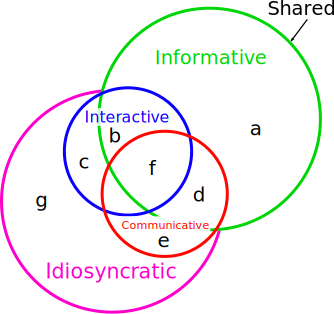
\includegraphics[width = 0.6 \columnwidth]{litreview/EkmanNvb.pdf}
\caption[The relationships between various types of non-verbal behaviours]{A set diagram showing the relationships between various types of non-verbal behaviour, adapted from Ekman and Friesen \cite{Ekman1969}, p. 57. This thesis aims to address communicative non-verbal behaviour, however an annotation's perception of communicative non-verbal behaviour is limited to subsets d and f.}
\label{FigureEkmanNvb}
\end{figure}

This thesis treats non-verbal communication and non-verbal behaviour as distinct concepts (similar to \cite{Krauss1996, Hall2012}), although these terms are sometimes used interchangeably \cite{Negi2009}. Non-verbal behaviours that convey information, called ``informative nonverbal behaviours'' by Ekman and Friesen \cite{Ekman1969}, are defined as acts that ``elicit similar interpretations among some set of observers''. Informative nonverbal behaviour includes both intentional and unintentional transfer of information. A separate issue is if a particular behaviour is communicative, in the sense that the behaviour was intended to be expressed by the sender to convey a particular message. As previously mentioned, Ekman and Friesen defined ``communicative nonverbal behaviour'' as ``those acts which are clearly and consciously intended by the sender to transmit a specifiable message to the receiver'' \cite{Ekman1969}. The terms \ac{NVC} and communicative non-verbal behaviour are treated interchangeably in this thesis and are characterised by their intentional expression \cite{Hall2012, Ekman1969, Lehtonen1981} and the use of a shared decoded meaning \cite{Hall2012, Ekman1969, Lehtonen1981, Wiener1972}. Similarly, Burgoon \etal \cite{Burgoon1996} limited the scope of \ac{NVC} to behaviours that ``are typically sent with intent, are used with regularity among members of a social community, are typically interpreted as intentional, and have consensually recognized interpretations''. An implication of this definition is that some non-verbal behaviours are not communicative \cite{Ekman1969, Engle1998}. Ekman and Friesen define a third type of non-verbal behaviour: interactive non-verbal behaviour which ``clearly modify or influence the interactive behaviour of the other person(s)'' \cite{Ekman1969}. These definitions of non-verbal behaviour are overlapping concepts; the relationship between them is shown in Figure \ref{FigureEkmanNvb}.

In contrast to the definition of \ac{NVC} above, it is popular to define \ac{NVC} in a much broader sense. This view considers communication to encompass all forms of information transfer, including unintentionally expressed behaviour and informative non-verbal behaviour. The broader definition was described by Fiske \cite{Fiske2010} as the ``semiotics school'' and the narrower \ac{NVC} definition (in the previous paragraph) as the ``process school'', with both approaches being necessary for appreciation of the field (see also \cite{Rozelle2006} for a broad literature review). Motley argued that, irrespective of the controversy of definitions, intentional and unintentional behaviour are distinct \cite{Motley1986}. The broad definition excludes the possibility of non-communicative non-verbal behaviour because any behaviour can be potentially interpreted, therefore ``one cannot not communicate'' as claimed by Paul Watzlawick \cite{Andersen1991}. However, this definition was considered to be over-broad by MacKay \cite{MacKay1972}, leading him to joke that by this broader definition, the study of \ac{NVC} would ``cover every interaction in the universe except the use of words!''

%Definition stuff \cite{Thirumalai2003}  \cite{Verderber2007} 
%NVC important \cite{Archer1977} \cite{Knapp1978} \cite{Nakatsu98} \cite{Proyas2004}

Mental state is a broad term for describing temporary mental conditions that have characteristic properties (see \cite{Perner1999} for a review). Mental states include emotion, attitudes, moods and cognitions \cite{Martin1990}. Many mental states manifest themselves as an outward expression and this expression can be intentionally modified to form a partly impulsive and partly controlled expression \cite{Frith2009}. This means mental state displays have both voluntary and involuntary aspects. However, some mental states are not necessarily externally observable, which distinguishes them from \ac{NVC} which is always externally observable. Emotions are a group of mental states that have connections to particular behaviours, have particular physiological manifestations (such as facial expression) and are also subjective experiences \cite{Frijda1986}. They tend to be triggered by stimuli, which are evaluated by a person, and spontaneously results in an emotion. Emotions are often expressed by facial expressions, vocal utterances, behavioural changes, and physical responses. The facial area is particularly important in emotion perception \cite{Ekman2009}. A facial gesture is a motion executed with the facial muscles and may be associated with mental states, emotion or \ac{NVC}. Emotion is an ill defined concept \cite{BeckerAsano2011, Shaver1987, Fehr1984}.
%which lead Fehr and Russell to quip, ``Everyone knows what an emotion is, until asked to give a definition. Then, it seems, no one knows''. 
However, this does not imply that there is no such thing as emotion, nor that it is not a subject worthy of investigation.

\ac{NVC} is a communication act that is only expressed in social situations. While some hold the view that emotions are also limited to social situations, others have observed that some forms of emotion can be expressed in non-social situations such as reading \cite{Mar2008} or dreaming \cite{Nielsen1991}. In a similar way to \ac{NVC} which typically lasting from a few seconds \cite{Lee1998} up to hours or longer, emotions can last from a fraction of a second (e.g. surprise) to hours or even longer (such as with empathy) \cite{Aaron1997, Verduyn2009}. The choice of clothing is an example of \ac{NVC} that has a long duration. A person's internal emotional state is sometimes manifested by facial expression, but the extent to which this is a direct relationship is controversial \cite{Azar2000}. At one stage Ekman claimed that six emotions (Anger, Disgust, Fear, Happiness, Sadness and Surprise) occurred across cultures \cite{Ekman1972} and called them ``basic emotions'', but later appended additional emotions to this list \cite{Ekman99}. He holds the position that different emotions are physiologically discrete and separate. This contrasts with approaches that describe emotions using continuous value labels \cite{Cowie2005}.

A social signal is `a communicative or informative signal which, either directly or indirectly, provides information about ``social facts'', that is, about social interactions, social attitudes, social relations and social emotions' \cite{Poggi2011}. Social signals include `interest, determination, friendliness, boredom, and other ``attitudes'' toward a social situation' \cite{Pentland2007}. The term social signals is used in animal behaviour\cite{Lin2005} and for human non-verbal behaviour \cite{Pentland2007}. The definition does not specify if the signals are necessarily verbal or non-verbal and many authors use the term ``non-verbal social signal'' for clarity \cite{Okwechime2011, Vinciarelli2008}. They are distinct from ``social behaviours'' which ``convey information about feelings, mental state, personality, and other traits of people'' and includes expressions of politeness and empathy \cite{Vinciarelli2008}.
%It is unclear if agreement is a social signal \cite{Poggi2011b} or rather a social behaviour \cite{Vinciarelli2008}.
%Emotion definition \cite{Frijda1991} \cite{Azar2000} \cite{Darwin2002} \cite{Fasel2003} \cite{Frith2009} 
The next section discusses the factors on which \ac{NVC} expression depends.

\section{What Factors Influence \ac{NVC} Expression?}
\label{BackgroundWhatFactorsInfluenceNvc}

There are many factors that influence human expression and perception, and specifically \ac{NVC}. If an automatic system is intended to be trained and deployed in a single environment, this will be of little concern. Although encoding based on motion is not sensitive to context, a system that is to recognise communicative intention for multiple people, or in multiple social and cultural situations, needs to account for contextual factors that can change how \ac{NVC} messages are interpreted\footnote{``From this example, it is obvious that in order to determine the communicative intention conveyed by an observed behavioural cue, one must know the context in which the observed signal has been displayed'' \cite{Pantic2008}}. \ac{NVC} is largely determined by the social situation in which it is used and therefore it is important to study \ac{NVC} in natural social situations \cite{Bavelas97}. Social context is also a factor that is used by human observers to interpret the behaviour of other humans, and humans are not reliable observers when this context is removed \cite{Hoque2009}. Social context, also referred to as social environment, ``encompass[es] the immediate physical surroundings, social relationships, and cultural milieus within which defined groups of people function and interact'' \cite{Barnett2001}. A waving gesture can be a greeting or a sign of distress depending on the context in which it occurs. Although cultural differences in expression exist for many \ac{NVC} signals, some signals have a similar appearance across cultures and social situations. There has been little research of the automatic recognition of \ac{NVC} messages that are specific to contexts, with most existing approaches only considering a single context or seek to generalise \ac{NVC} across different contexts.

%Context important, don't see how this particular paper is relevant \cite{Mower2009}

Factors which influence the expression and interpretation of human behaviour include:

\begin{itemize}
 \item culture (this is discussed in depth in Section \ref{BackgroundCrossCulture}),
 \item gender,
 \item personal style,
 \item personality and
 \item social situation.
\end{itemize}

People naturally vary in expressiveness; some individuals being animated while others being comparatively inexpressive \cite{Afzal2009}. Buck claimed that encoding and perceiving accuracy for \ac{NVC} was dependent on gender, personality and age \cite{Buck1979}. However, these studies assume that there can be ``correct'' and ``incorrect'' interpretations of emotion and \ac{NVC}. This view seems questionable because the use of posed behaviour does not necessarily imply that the samples are directly associated with an objective, exemplar basis of human behaviour. However, the study does highlight the differences in the interpretation. Gender difference in expression style was investigated by Morrison \etal \cite{Morrison2007}, who found there were specific facial movement styles that could be used by humans to identify gender. Some medical conditions, such as schizophrenia spectrum disorder, can change how \ac{NVC} is expressed \cite{Brune2009}. %A study of \ac{NVC} expression in wild chimpanzees also shows individual and age based variations in gesture repertoire \cite{Hobaiter2011}, which is notable because chimpanzee emotional behaviour is comparable to human behaviour except for the lack of verbal communication. 
All these studies provide evidence that there are individual variations in how \ac{NVC} or emotion is expressed.

% 
When humans experience emotion, the emotion often manifests itself in body language and facial expression. Emotion expression is based on many factors. The mapping from emotional state to emotional expression can be thought of as a set of rules, according to Ekman and Friesen \cite{Ekman1975} with each culture having a specific set of encoding rules. Other researchers have extended this idea to specific social situations having distinct display rules \cite{Feldman1991, Brinton2007} that encode the internal state. For this reason, a person expressing an emotion is sometimes referred to as an ``encoder''.
%Matsumoto \etal \cite{Matsumoto08} conducted cross cultural studies and found display rules had commonalities and differences across various cultures. However, cultural differences in gaze aversion was described in terms of cultural rules by McCarthy \etal \cite{McCarthy2006}. 
Research related to the effect of culture is described in more depth in Section \ref{BackgroundCrossCulture}.
Studying the mapping from emotion to expression across cultures can be challenging. To demonstrate that cultural display rule differences or similarities exist, the underlying emotions used must be shown to be equivalent across cultures. \ac{NVC} expression may also have encoding rules which are analogous to encoding and display rules. %However, the terminology of encoding and decoding rules is less commonly applied to \ac{NVC}.
Just as emotions have shared social norms and expectations that are used when managing and modifying emotional displays in different social circumstances, \ac{NVC} expression is also dependent on social circumstances.

%Cross species: \cite{Fridlund94}, \cite{Darwin2002}, \cite{Ekman2009}, \cite{Hobaiter2011} 
%Personality and career choice are associated \cite{Vuust2010}, which leads to personality based perception differences.
%Subjects given shock or no shock, then asked to rate \ac{NVC} of other subjects \cite{Lanzetta1970}, 
%Classifying full body motion with emotion labels \cite{Bernhardt07}, 

Social situation is also a factor in \ac{NVC} and emotion expression. The effect of social situation itself shows cultural, gender and personality differences \cite{Argyle1994} making these factors interdependent. Social situation is significant for capturing a corpus of \ac{NVC} behaviours, because the situation in which the recording takes place affects the type and frequency of observed behaviours. It is often convenient to record posed data, because behaviours directly correspond to pre-determined labels and little time is wasted on recording uninteresting behaviour\footnote{Even if acted data is considered as having no social context, the absence of a social context is a factor in \ac{NVC} expression.}. All human behaviour occurs in a situational context, although acted behaviour may be a special case in that it has a context in terms of social interaction with the audience. Unfortunately, human behaviour is significantly different in posed situations when compared to spontaneous behaviour. Cowie \cite{Cowie2005} argues that the use of posed data cannot be completely excluded but posed data should not be used uncritically. There has been a recent shift in the automatic human behaviour recognition community to use natural data, rather than posed. However there is a wide range of approaches to collect so called ``natural data'' to the point that the word can be misleading. The definition of natural language proposed by Stubbs \cite{Stubbs1983} can be adapted to suit \ac{NVC}: that natural \ac{NVC} occurs ``without any intervention from the linguist [or experimenter]'' and ``is spontaneous in the sense of unplanned, and which is composed in real time in response to immediate situational demands''. Applying this to \ac{NVC}, this definition excludes posed examples of \ac{NVC}, as well as \ac{NVC} based on artificial tasks, stages scenarios, role play tasks or experimenter controlled stimuli (such as a ``Wizard of Oz'' apparatus). The issue of social situation is discussed in more depth in Section \ref{BackgroundSocialContextUsedInTwoTalk}. Just as the expression of \ac{NVC} depends on many factors, the perception of \ac{NVC} is also dependent on multiple factors. These will be discussed in the next section.

%Language word order doesn't seem to change \ac{NVC} order \cite{SusanGoldin2008} although the situation in mime is rather different to natural?

\section{Perception of \ac{NVC}}
\label{BackgroundWhatFactorsInfluenceNvcPerception}
\label{BackgroundPeopleVaryInExpression}

The interpretation of emotion is based on various contextual factors, such as culture, social situation, age, etc. Building on the idea of encoding rules, Argyle \cite{Argyle1994} suggested there exists a mapping from observable behaviour to a meaningful interpretation and termed this mapping as ``decoding rules''. Several studies have found context and conditions that affect perception of human behaviour, including \ac{NVC} and emotion. Terracciano \etal \cite{Terracciano2003} found there is a relationship between personality and emotion perception. Matsumoto \etal \cite{Matsumoto2000} claimed that accuracy in emotion recognition was correlated with personality measures such as Openness and Conscientiousness. Personality differences of experimental participants, such as neuroticism, were associated with different subject gaze patterns being observed during an emotion recognition task \cite{Perlman2009}. However, little work has been conducted in the association between personality differences and \ac{NVC} perception. Behaviour mirroring, which is the tendency of people to adopt the behaviour of another person in a conversation, is more pronounced in people who had tested highly on an empathic personality measure \cite{Chartrand1999}. Lanzetta and Kleck \cite{Lanzetta1970} found that a person's \ac{NVC} perception ability was related to personality and that highly able subjects were themselves difficult subjects for others to read. All these findings provide evidence that both personality and individual style have a role in the perception of emotions and \ac{NVC}.

% The role of personality is thought to influence the choice of career, although that role not well understood \cite{Vuust2010}. 

Another factor in behaviour perception is gender. Vassallo \etal \cite{Vassallo2009} found that gaze patterns during evaluation of emotion were different between genders and that females arrived at a judgement faster than males. Gender based differences in annotator judgements have also been observed in several studies \cite{Buck1979, Terracciano2003, Abrilian2006}. Context can be a factor in perception, but this may still be specific to certain cultures and personalities. The way face images are viewed can affect perception. The presence and expression of surrounding faces changes the judgement of a central face in some cultures but not others \cite{Masuda2008}. Goren and Wilson \cite{Goren2006} found that intense, posed emotion is easier to categorise than weak, posed emotion, as well as finding that emotions are harder to rate accurately if viewed by peripheral vision. Perception of emotion was significantly affected by the level of familiarity with the person being observed \cite{Hoque2009}. El Kaliouby \etal \cite{ElKaliouby03} found that while basic emotions (Ekman 6 and contempt) were almost instantaneously recognized by humans, temporal context improved human recognition for complex emotions, such as interest, boredom, confusion, etc. All these factors make annotation a challenging task, because these variables cannot be easily controlled while maintaining the naturalness of the data. Using multiple annotators and finding a consensus is one common approach. However, personality, relationship and familiarity of people in a social situation are important contextual factors in the expression of \ac{NVC} and using a consensus score discards this aspect of context.

%Perception of hearing is coupled with sight \cite{McGurk1976}

%\cite{Fernandez-Dols2003}, \cite{Reidsma2008Thesis}, \cite{Reidsma2008}, \cite{Eckhardt2009}, \cite{Frith2009}, 

%Perception in context \cite{Archer1977}, \cite{Cowie1999}, 

%\subsection{Models of \ac{NVC} and Emotion}

%Why care about this? Is later discussion sufficient?

%Taxonomies: \cite{Ortony1988}, \cite{Bavelas97}, \cite{Cowie1999}, \cite{Scherer1999}, \cite{Darwin2002}, \cite{Hillard03}, \cite{Jandt2004}, \cite{Darn2005}, \cite{Harrigan2005}, \cite{Matsumoto2006}, \cite{Verderber2007}, \cite{Zara2007}, \cite{Vinciarelli2008}, \cite{Cowie2009b}, \cite{Ekman2009}, \cite{GaticaPerez2009}, \cite{Knapp2009}, \cite{Mower2009}, \cite{Truong2009}, \cite{Wollmer2009}, \cite{Griggs2010}, \cite{Hobaiter2011}.

%Labels: Basic emotions \cite{Ekman1972}, \cite{Ekman1975}, \cite{Matsumoto1990}, \cite{Argyle1994}, \cite{Rosenblum1996}, \cite{Ekman99}, \cite{Cohen2000}, \cite{Marsh2003}, \cite{Feng2005}, \cite{He2005}, \cite{Hong2006}, \cite{Kanaujia2006}, \cite{Datcu2007}, \cite{Moore07}, \cite{Jack2009}, \cite{Moore2009}, \cite{Vassallo2009}, \cite{Fanelli2010}, \cite{Griggs2010}, \cite{Jeni2011}, \cite{Pfister2011b}.

%Abstract scales \cite{Ekman99}, \cite{Cowie2000}, \cite{Liscombe2003}, \cite{Fontaine2007}, \cite{Grimm2007}, \cite{McRorie2007}, \cite{Kanluan2008}, \cite{Truong2009}, \cite{Nicolaou2011}

\section{Supervised Learning for \ac{NVC} Recognition in Video Sequences}

One of the aims of this thesis is to create an automatic system to perform facial, intentional \ac{NVC} recognition, based on previously observed examples of behaviour. As well as directly relevant studies in the field of automatic behaviour recognition, this review discusses research from other fields if they are particularly relevant to this thesis. Video recording of \ac{NVC} has been previously been used in the behavioural sciences \cite{Matsumoto1991}, as well as studies into facial biometrics \cite{Goswami2010}, automatic lip reading \cite{Ong2011}, character animation \cite{Bickel2008} and affective computing systems \cite{Pantic2008, Bartlett2010, Zeng2009}.

Based on video of facial behaviour, training data and manually annotated labels are used to create a model; this process is known as supervised learning. Based on the model, labels for unseen samples can be automatically predicted. The input data and labels are digitised to allow computers to process the input data. Supervised learning is often divided into \featureGeneration, which provides a set of higher level features, followed by a classification technique. 
%Feature generation is also called a feature transform methods, feature construction or feature extraction in the literature \cite{Torkkola2003}. 
Given an ideal training set with total coverage of the feature space, the use of \featureGeneration and a sophisticated classifier would not be necessary; nearest neighbour classification \cite{Cover1967} would be sufficient. However, the available data sets contain a limited number of samples and also contain noise. To improve the performance of a classifier on limited training data, visual changes that are not relevant to the task at hand should be separated or removed from the input data. This improves the robustness of an automatic system and is usually achieved by manual design of the system or by feature selection. This is often accomplished by \featureGenerationComma which aims to improve robustness and reduce the quantity of training data required. Almost every application of supervised learning uses \featureGeneration which transforms the data into a ``higher level'' representation; common approaches are described in Section \ref{BackgroundEncodeFacialInfo}. The \featureGeneration technique used in an automatic system is usually selected manually. There are also many supervised classification methods (described in Section \ref{BackgroundSupervisedClassification}). The type of classifier used may dictate which \featureGeneration approach is optimal and visa-versa, so these issues are closely interrelated. %Manually selecting an appropriate \featureGeneration method and classification technique is necessary because prior knowledge of the problem domain must be exploited \cite{Wolpert1996}.

\begin{figure}[tb]
\centering
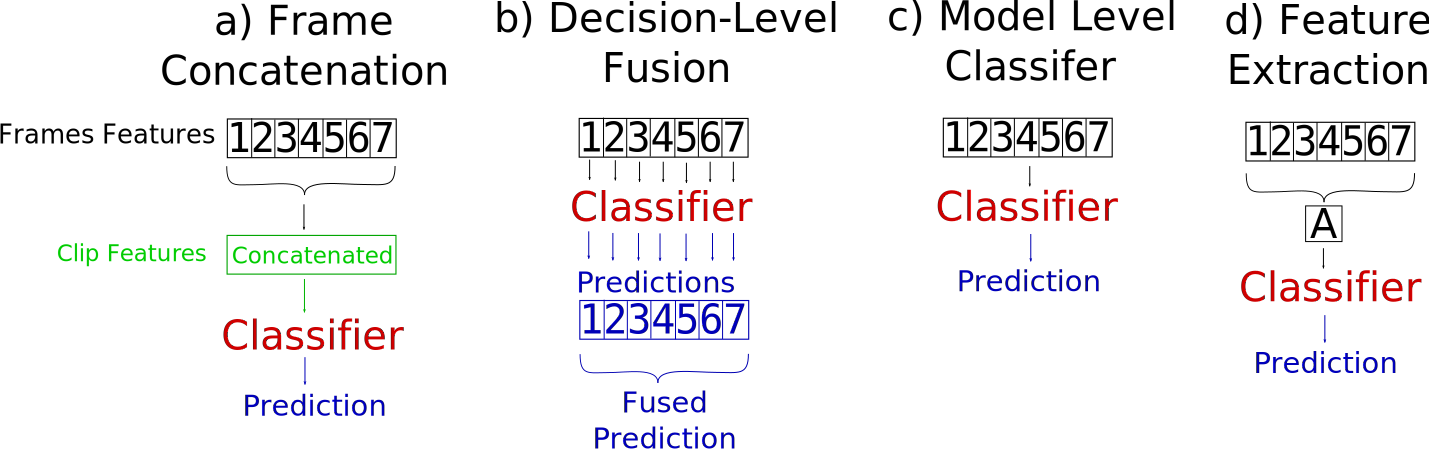
\includegraphics[width = 0.9 \columnwidth]{nvcclass/VideoRecognition.pdf}
\caption[The common approaches to using a classifier with video sequences.]{The common approaches to using a classifier with video sequences. \FeatureGeneration and machine learning have a different role in each case.}
\label{FigureVideoRecognition}
\end{figure}

Once \featureGeneration has been performed on a sequence of video frames, the variable length of examples and temporal nature of a video must be considered to achieve effective automatic recognition performance. This section only considers the processing of visual information and does not consider the issues of fusing audio and video, which is beyond the scope of this thesis. A temporal \ac{NVC} signal can be recognized using data from multiple observations by using \dataFusion which encodes temporal variations early in the recognition process. Alternatively, a model based recognition system may be used, which deals with temporal variation at a higher level.
%Data fusion, or more strictly speaking ``information fusion'', is the exploitation of ``the synergy in the information acquired from multiple sources [...] such that the resulting decision or action is in some sense better [...] than would be possible if any of these sources were used individually [...]'' \cite{Elmenreich2002}. Data fusion is usually used to combine different modalities of data, but may also be used to combine features of a single modality \cite{McKee1993, Zhang2004, Dietrich2001, LakshmiDeepika2009}. 
\DataFusion of multiple observations that were acquired at different times is referred to as ``temporal fusion'' \cite{Varshney1997, Ko2008}. 
%There are different levels of fusion, including: sensor level fusion, feature level fusion and post classification ``expert fusion'' \cite{Poh2010}. Post classification fusion methods include match score level, rank level or decision fusion methods \cite{Poh2010}. Many of these approaches can also be considered as temporal fusion. 
These \dataFusion approaches will now be described in more detail, in the context of temporal, uni-modal video based recognition (see also Figure \ref{FigureVideoRecognition}).

\begin{itemize}
 \item Sensor level feature extraction consolidates raw video image images into a combined raw feature. This is rarely used in the context of human behaviour recognition.
 \item In one form of temporal feature extraction, all frames can be concatenated and directly used by a standard classifier. This can be directly applied to fixed length examples. (Figure \ref{FigureVideoRecognition} a) Frame concatenation is a special case of feature-level encoding. If different modalities are sampled at different frequencies or if samples are of varying length, re-sampling can enable feature concatenation.
 \item Decision level fusion: Each frame can be classified individually using standard machine learning, then the predictions combined and used in a second classifier step to provide an overall overall clip prediction. Decision level fusion may use multiple samples from one or more types of sensor \cite{Vakayallapati2011}. (Figure \ref{FigureVideoRecognition} b). Variants of decision level fusion include rank level fusion and match score fusion. Rank level fusion: multiple recognisers rank possible hypotheses and these rankings are combined to form a final label. Match score fusion: prediction labels are provided by multiple recognizers based on multiple, individual observations and these labels are then combined to generate information for decision making.
 \item Model level recognition: individually encoded frames can be directly used by some types of machine learning methods. The order of the frames in the clip can be used (as typically done with \ac{HMM}, \ac{CRF}) or ignored (e.g. as Nearest Neighbour or \ac{MIL}). (Figure \ref{FigureVideoRecognition} c)
 \item Feature extraction methods 
 %are often used to combine samples of different modalities, but may also be used to fuse features of the same modality \cite{Zhang2004}. They also may 
 encode how low level observations vary over time in a way that can be interpreted by a classifier. Frames can be summarised or combined into a fixed length vector, then classified using a standard supervised learning technique. This approach is used in Sections \ref{SectionTemporalFeatures} and \ref{SectionClipFeatureExtraction}. (Figure \ref{FigureVideoRecognition} d). One simple approach is to concatenate frames into a single vector (Figure \ref{FigureVideoRecognition} a). 
\end{itemize}

Concatenating frame based shape or appearance features before classification is rarely used because videos of varying lengths cannot be directly compared and the approach tends to be sensitive to the speed of activity in the video. For varying length videos, one approach is to re-sample the frame features to produce a fixed length vector, as done by Pfister \etal \cite{Pfister2011}. However, the feature vector can be sensitive to whether an event of interest occurs at the start of a clip, or at the end; this may not be desirable if the occurrence of the event at any time is of significance. This is not an issue for approaches that use unsegmented videos \cite{Oikonomopoulos2011}.

Feature extraction is a popular group of approaches that combine one or more frames into a feature vector, usually of fixed length. Multimodal feature extraction by up-sampling video features and concatenating them with audio features was performed by Petridis and Pantic \cite{Petridis2008, Petridis2009, Petridis2011} and others \cite{Potamianos2001, McCowan2005, Nicolaou2011b}. This can increase the dimensionality of the data, which may reduce the performance of the final system. Other feature-level extraction approaches try to encode temporal variations \cite{Dietrich2001}. Valstar \etal \cite{Valstar2006} calculated the mean and maximum change in the displacement and velocity of feature points during facial deformations, which is a form of temporal feature extraction at the feature level. This reduces the dimensionality of the data while hopefully retaining temporal information about the face. In a similar way, face deformation based on heuristic features was encoded by taking the variance of each feature by Datcu and Rothkrantz \cite{Datcu2007}. As well as using the mean and standard deviation of features in a clip, Petridis and Pantic \cite{Petridis2008} fitted a quadratic curve to each feature component to encode temporal variation. Most of these approaches use geometric deformation based features, however temporal encoding has also been used for texture and audio. Aligned facial textures were compared using the mean shape and appearance features by Fang and Costen \cite{Fang2009}, however, using only the mean does not encode temporal variation information. For audio features, Grimm \etal \cite{Grimm2007} used seven simple statistical measures on the features, as well as the feature's first and second derivatives, which may be useful in encoding the rate of feature variation.

Fusion after matching combines the predictions from multiple classifiers to form a final decision. This is also known as match score fusion and is a form of decision level fusion. This may be used to combine different types of features, different modalities, predictions from independent video frames or the predictions of different classification methods. The most popular decision level fusion methods are the ``sum rule'' and rank based voting \cite{Kittler2003}. The sum rule takes the class dependent average of the predicted probabilities and selects the class label with the highest score. Rank based fusion has each classifier rank each label and these are combined, using one of several approaches, to form a final prediction. One ranking fusion method is majority voting, which takes the highest probability label from the classifiers and the label with the highest proportion is taken as the fused prediction. Audio and visual decision level fusion has been used in many studies \cite{Vakayallapati2011, Poh2010, Petridis2008, Petridis2010, Kanluan2008}. Pfister \etal \cite{Pfister2011b} used majority voting to combine predictions of three types of classifier for visual features. Three different rank based fusion methods were compared by Akak{\i}n and Sankur \cite{Akakin2011} to combine different types of visual features, although there were no appreciable performance differences between the ranking approaches. Audio and video modalities were fused at the decision-level by the sum rule by Petridis and Pantic \cite{Petridis2008}. The sum rule allows the decisions to be weighted to change the emphasis on different modalities, as done manually by Kanluan \etal \cite{Kanluan2008}, or automatically by \ac{LLR} fusion as performed by Lucey \etal \cite{Lucey2009}. Oikonomopoulos \etal \cite{Oikonomopoulos2011} used voting to combine information from different human action models. Ko \etal \cite{Ko2008} showed that dynamic time warping can result in a higher performance than a \ac{HMM} approach for recognizing hand gestures based on multi-sensor fused data. Based on these studies, combining multiple modalities with decision-level fusion often results in a large increase in performance compared to a single modality (although exceptions exist to this pattern \cite{Nicolaou2011b}) and often has recognition performance advantages over feature level fusion (although some studies have shown that the performance using feature fusion is comparable to other approaches in some cases \cite{McCowan2005, Petridis2008}).

Rather than combining features or decisions, feature vectors from multiple frames may be considered directly by a machine learning algorithm. There are two general classes of algorithms: sequential temporal model classifiers (e.g. \ac{HMM}, \ac{CRF}) that consider an ordered group of items, and ``unordered set'' classifiers (e.g. \ac{MIL}) which considers a set of items in which the ordering is not considered. These are among the most popular approaches in the recognition of human behaviour. They are discussed in more depth in Section \ref{BackgroundSupervisedClassification}.

Petridis \etal \cite{Petridis2010} used a different approach to combining multimodal information by using the audio mode to predict the expected visual features and visa-versa. A positive prediction is made if the predicted features match the observed features and this approach exceeded feature level fusion performance for laughter vs. speech discrimination.

\thesiscomment{DISCUSS going via a known intermediary representation e.g. FACS? Emphasis similarity in approach?}

%This section has examined different high level frameworks for human behaviour recognition, and in particular how \featureGeneration and classification are related. The next section will examine the common \featureGeneration techniques.

\section{Encoding Facial Information}
\label{BackgroundEncodeFacialInfo}

\thesiscomment{DISCUSS what part of the body are we trying to encode? ignoring the audio?}

\thesiscomment{DISCUSS features are important \cite{Shan2009} \cite{Yang2009}}

% Almost all automatic approaches use \featureGeneration to encode information about human behaviour. This thesis focuses on facial features, because the facial area is rich in emotion and communication information \cite{Ekman2009}. However, \ac{NVC} signals may be communicated by many other non-facial means, as described in Section \ref{BackgroundHowIsNvcExpressed}. 
Facial features encode shape information by shape or appearance changes, or by combining both types of information. The common approaches will now be described and some of their strengths and weaknesses will be discussed.

\subsection{Encoding Behaviour Using Appearance Based Features}

Changes in facial expression often cause changes in facial appearance due to wrinkles, deformations that change the visibility of the inside of the mouth, etc. However, to make effective use of limited training data, images are typically aligned to a canonical head position or to a canonical head shape. This ensures correspondence between local areas of different face images is maintained and the effect of head pose changes and translation is reduced, making the method much more effective. An alternative is to use changes in an overall image without using alignment which would be effective in encoding head movements, as done by Escalera \etal \cite{Escalera2009}, but this cannot accurately encode subtle facial deformations. Some papers on emotion recognition deliberately ignore the image alignment problem and instead focus on the robustness of later steps in the automatic process \cite{Shan2009}. %Image alignment approaches can be broadly split into part based (or landmark) detection based methods and methods that employ an overall face model \cite{Yang2009b, Boom2010}. 

Some approaches to face alignment begin with interest point detection; the face can be subsequently re-scaled or affine transformed to a canonical alignment \cite{Zhu2009b}. Yang \etal \cite{Yang2009b} used SIFT interest points and a similarity transform. Yang and Bhanu \cite{Yang2011} found point correspondences between images using the SIFT-flow technique and removed shape information in the alignment process. This would help to reduce the effect of identity in emotion recognition. Zhu \etal used Lucas-Kanade based local correspondences to perform a non-rigid transform \cite{Zhu2009b}.

Other approaches for face alignment use whole face detection or a more general model for the overall face shape or colour. The most popular basis for face alignment is the Viola and Jones object detector \cite{Viola2002}, with several studies using this as a basis for image alignment \cite{Kanluan2008, Bartlett2006, Moore07}. Skin colour based detection was used by Feng \etal \cite{Feng2005} to align images; this was robust to illumination changes and, to a limited extent, to pose changes. Some models attempt to fit an expression model (which is often inspired or validated using \ac{FACS} \cite{Cosker2010, Ahlberg2001}) or a shape and appearance model to the observed face, or be limited to variations of shape, head position and pose. Shape based approaches will be discussed below in more depth but there are a few studies that use face models for the purposes of alignment pre-processing before extracting appearance based features. Pfister \etal \cite{Pfister2011} used an active shape model to achieve alignment. \ac{AAM}s may also be used for normalisation \cite{Lan2009} but it common to use the model's parameterisation directly for recognition, rather than to the normalised face as a preprocessing step. Dornaika and Davoine \cite{Dornaika2005} used a 3{D} head model to not only normalise the face translation and pose, but also to remove shape information from the features. Other whole face based approaches avoid shape models and use image information more directly to determine an appropriate alignment transform. Visser \etal \cite{Visser1999} used \ac{PCA} on training images to perform lip localisation, however this was computationally expensive. The alignment transform may be directly found by the affine transformation of an input image on to a canonical image, by maximising pixel intensity correlation \cite{Tzimiropoulos2011}. Rudovic and Pantic \cite{Rudovic2011} used a shape constrained Gaussian process to fit a facial point based model while retaining an anatomically plausible shape. Dhall \cite{Dhall2011} \etal used \ac{CLM} to normalise head positions for emotion recognition, which fits a parameterised model to landmarked positions based on an ensemble of local feature detectors.

Image alignment is intended to remove appearance variations caused by face translation and pose. Often a simple affine or re-scaling transformation is employed. However, natural conversations contain extreme head poses. Until recently, alignment of images based on detection of facial features over a wide range of head poses was an unsolved problem \cite{Zhu2012}. An affine transform from an input image to a canonical face is challenging because of self-occlusions \cite{Yang2011}. For these reasons, using an approach that depends on face alignment to frontal view may fail at extreme poses.

Once the input image has been aligned, appearance features may be extracted that correspond across multiple faces. Two broad approaches are employed: holistically encoding pixel information or part based methods. These types of appearance based features will be discussed.

\begin{itemize}
 \item Holistic approaches use dimensionality reduction techniques to encode changes in overall pixel intensity. Visser \etal \cite{Visser1999} and Seguier \etal \cite{Seguier2002} performed \ac{PCA} on the lip region of interest. Chew \etal \cite{Chew2012} used shape normalised textures to recognise \ac{AU}s and compared this method to local texture approaches under the effect of noise, on four public datasets. Texture descriptors may be applied to every pixel in the image as the basis for classification \cite{Bartlett2006, Moore07}. If a transform is applied on a per pixel basis, the feature vector may become excessively large. Using histograms of texture reduces the representation to a manageable size and also reduces spatial sensitivity, which may be advantageous in improving robustness to insignificant differences in face shape. Kanluan \etal \cite{Kanluan2008} performed \ac{DCT} on lip and eye pixels. He \etal \cite{He2005} used \ac{ICA} on facial images to find independent modes of variation. These methods are useful for finding low frequency spatial information, which is often more relevant than using individual pixels or high frequency components, which correspond to very small areas or very small changes that are unlikely to be significant on their own. However, changes in individual components of these methods typically correspond to a global change in the region of interest and would involve multiple muscle movements. It is likely that features that do not isolate changes based on individual facial muscles would be sub-optimal. %This is due to the inter-person correspondence between muscles for facial expression, as encoded by \ac{FACS}, is closer in similarity than for the face's visual appearance (due to interpersonal differences e.g. face shape, wrinkles, facial hair, etc).

 \item Rather than encode an overall image, a feature can attempt to encode local texture information near points of interest. This makes localised changes in the face affect only some feature components. As mentioned, this decoupling of the different parts of the face may be useful because it is expected that local changes in the face are useful for recognition. Texture descriptors may be applied to limited regions and encoded using histograms, which provides a more compact representation \cite{Feng2005, Shan2009, Pfister2011, Moore2009, Yang2011, Tingfan2012}. There are several popular texture descriptors used in facial recognition, particularly Gabor filters (\cite{Bartlett2006, Wang2006, Rose2006}) and \ac{LBP} features (\cite{Feng2005, Shan2009, Yang2011, Moore2009}). Recent work has considered layers of texture descriptors. Senechal \etal \cite{Senechal2012} used \ac{LGBP} histograms for \ac{AU} recognition, which are \ac{LBP} operators applied to Gabor filtered images. Tingfan \cite{Tingfan2012} compared using a single layer (Gabor energy filters and \ac{LBP}s) with double layer texture filtering, finding that double layer is more effective in multiple data sets.
%These techniques are effective for constrained, basic emotion recognition. 
\ac{LBP}s were extended to encode temporal variation, and named \ac{LBP}-\ac{TOP}, by Pfister \etal \cite{Pfister2011}, however considering changes on a short time scale, such as consecutive frames, may not be optimal for all facial gestures. \ac{LBP} features are also noted for being relatively robust to illumination changes, and in some forms are also robust to rotation. Other approaches include edge based texture descriptors, such as Moore and Bowden \cite{Moore07} using Canny edge detection to form chamfer images as the feature extraction step. Yang and Bhanu \cite{Yang2011} used \ac{LPQ} features that exceeded \ac{LBP}s performance for emotion recognition on acted data. Jiang \cite{Jiang2011} extended the \ac{LPQ} to consider temporal variation (\ac{LPQ}-\ac{TOP}) and found it exceeded performance of \ac{LBP}-\ac{TOP}.
\end{itemize}

Donato \etal \cite{Donato1999} compared many appearance based approaches and found Gabor features with \ac{ICA} dimensionality reduction was the most effective for facial expression recognition.

\thesiscomment{DISCUSS Facial action dynamical models \cite{Dornaika2005}? combines steps into one?}

As previously mentioned, images are usually aligned before appearance features are extracted. While these features have been successfully employed for many constrained datasets, appearance based features are only as good as the face alignment process, which may be problematic for extreme head pose. Appearance based features encode information about the face that can be used as the basis of classification, but also includes information that is not necessarily relevant. Depending on the behaviour under consideration, these irrelevant appearance differences include facial hair, wrinkles, skin colour, glasses, etc. Although some emotions are associated with colour change in the face, colour information is rarely considered because differences in skin colour make interpersonal facial colour comparisons problematic. Various approaches can be employed to remove personal differences in features (Section \ref{SectionPostProcessingFacialFeatures}). Appearance features also may be non-optimal if significant facial movements occur that do not cause a detectable change in local appearance. 
%Wrinkles only form in larger facial movements and small deformations may be ignored by texture descriptors. 
Facial deformations are expected to be important for automatic \ac{NVC} recognition. For this reason, many approaches attempt to encode face shape directly. The next section will consider these types of features.

\subsection{Encoding Behaviour Using Shape Based Features}
\label{BackgroundTemplateTracking}

Shape based features are used to encode information about facial deformation and head pose. Because many human \ac{NVC} signals are based on body and face gestures, encoding the shape captures this type of information. Shape based features usually involve fitting a model to an observation image. The body part selected for feature extraction and sophistication of the model depend on the task that is being attempted. Various approaches have used simple head models that can encode head pose changes, or both the pose and facial expression. Yang \etal \cite{Yang2009} used a simple 2{D} model to encode the face. Chen and Ji \cite{Chen2011} apply \acl{DBN}s to combine facial tracking with expression recognition in a hierarchical framework. Zhu and Ramanan \cite{Zhu2012} used mixtures of trees with a shared pool of parts to localise faces, estimate pose, as well as locate points of interest in unconstrained photographs. Petridis \etal \cite{Petridis2009} used a 3{D} cylindrical model to track the face, with six degrees of freedom corresponding to translation and rotation. This would not encode facial expression but should be sufficient for gestures based on overall head movement. Dornaika and Davoine \cite{Dornaika2005} used a more sophisticated model including deformation to fit facial expression. Zeng \etal \cite{Zeng2006} used a {3D} model based visual tracker for expression recognition. However, complex models are computationally demanding, have higher training requirements and usually require advanced methods to fit the model reliably and robustly. Other approaches use 3{D} shape based on structured light capture systems for emotion recognition \cite{Sandbach2011, Fanelli2010b, Chen2011}. The face is of most interest for \ac{NVC} recognition, but may be complemented by other parts of the body. Occasionally other parts of the body are used for model fitting and recognition, including the shoulders \cite{Petridis2009} or the overall body pose \cite{Bernhardt07}.

Some studies use a hybrid approach to extract a model, such as \ac{AAM}s, and then use only the components corresponding to the shape for recognition \cite{Girard2011}. This has been done by heuristic feature extraction from \ac{AAM} features \cite{Datcu2007}, as well as distance ratios of points of interest \cite{Tang2007}. Other approaches use both shape and appearance, which will be discussed in the next section.

Another approach is to treat the body as independently moving parts, localise the position of each part in the frames of the video sequence and use this information directly, or fit a model based on the independent parts. This is conceptually simpler than fitting a complex model with inter-dependent parts. However, position and motion of areas of the body can provide information for the movement of nearby body areas and this is not used by tracking independent points of interest. Tracking attempts to localise a feature of interest in a series of video frames. Tracking uses the assumption that a point of interest has a locally constant appearance. This separates motion from other non-shape changes in the video. However, large changes in appearance caused by pose changes or occlusions make tracking spontaneous videos difficult. Lucas and Kanade  \cite{Lucas1981} proposed a method based on minimising the least squares difference of a training patch to a test image by gradient descent. However, it can suffer from local minima, noise and occlusions which can lead to tracker drift. An alternative is to use a particle filter based approach, which is robust to noise by using multiple hypotheses of tracker position \cite{Isard1998}. However, this approach does not scale well to high dimensionality. This was addressed by partitioning the model space components into groups by Patras and Pantic \cite{Patras2004}. This tracking method is limited to small head pose changes of approximately 20 degrees \cite{Valstar2012}. This is because of the change of appearance caused by head rotation breaks the assumption of an unchanging local appearance near to a tracked point of interest. Chew \etal \cite{Chew2012} used a \ac{CLM} to detect \ac{AU}s, which uses detections of facial points of interest as the basis to fit a shape model. \ac{CLM}s \cite{Cristinacce2008} are similar to \ac{AAM}s but generate likely feature templates that correlate with the target image, rather than trying directly fitting a model to pixel intensities. Baltrusaitis \etal \cite{Baltrusaitis2012} extended \ac{CLM}s to {3D} and applied it to head pose tracking. Liwicki \etal \cite{Liwicki2012, Liwicki2012b} proposed a kernel \ac{PCA} method, which retains desirable properties of \ac{PCA} while being robust to outliers; this encodes behaviour as shape information. They applied the method to different computer vision problems, including visual tracking and found it was better than 4 other state-of-the-art tracking methods in most video sequences.

The approach used in this thesis is the pre-existing tracking technique proposed by Ong \etal \cite{Ong2009} called \acf{LP} tracking; this method encodes behaviour as face shape changes. This method learns a linear mapping from intensity changes in a sparse template to a tracker positional offset. The tracker is trained on multiple training frames which improves its robustness to appearance change, including an amount of head rotation. The maximum tolerated head rotation is not known, but it is suitable for tracking spontaneous human behaviour. The tracker does not automatically recover from occlusions, so the tracker must be manually re-initialised when a feature becomes visible. This could be addressed by incorporating an automatic feature detector to re-initialise tracking positions. This tracking process results in the facial behaviour being encoded as a series of shape deformation frames. The technical details of \ac{LP} tracking are discussed in Appendix \ref{BackgroundLpTracking}.

Tracking data encodes facial deformation changes and can be used directly for behaviour recognition. Tracking is not effective in areas which contain relatively little local texture, such as can be seen in puffed cheeks. Tracking has often been applied to estimate optical flow and this approach encodes the overall face deformation. This method was used to recognise emotions by Rosenblum \etal \cite{Rosenblum1996}. Overall head translation information is usually unrelated to facial expression and is often separated from facial deformation information. However, differences in face shape can prevent direct comparison of optical flow features generated on two different people. Also, optical flow based approaches tend to be sensitive to head rotations and require a constant frontal view of the face. Other approaches use tracking of points that corresponds to known positions on the face. This correspondence makes inter-person comparison of deformations easier. Tracker movements are caused by both head movement and expression changes, but this is not ideal for existing machine learning techniques. Head motion was separated from deformation changes using \ac{PCA} by Petridis and Pantic \cite{Petridis2008}. Another way to improve person independent recognition is to remove the effect of face shape by mean shape subtraction \cite{Tax2011}.

%Direct use of tracking features? \cite{Nicolaou2011}

\subsection{Encoding Behaviour Using Both Shape and Appearance}

The previous sections have discussed features that encode either the shape or the appearance of human \ac{NVC} and emotion. To guide future work, it may be useful to know which approach is most effective, or if these approaches can be combined effectively. Some papers compare shape features to appearance feature approaches and this provides insight into the best approach for encoding behaviour. However, comparisons of specific techniques do not rule out the creation of superior \featureGeneration techniques. Lien \cite{Lien1998a} compared three methods (feature point tracking, dense flow and texture descriptors) for emotion recognition of posed examples and found dense optical flow is most effective. Both Fanelli \etal \cite{Fanelli2010} and Akak{\i}n and Sankur \cite{Akakin2011} had similar findings, with optical flow or tracking being effective but optical flow or tracking combined with appearance and shape demonstrating a higher performance. However, optical flow techniques are susceptible to head rotation, which commonly occurs in spontaneous behaviour. Some model based methods extract both shape and appearance information which can be used for recognition. A popular approach for facial analysis is an \acf{AAM} \cite{Cootes1998}. This has been used for emotion recognition and studies have found that while shape is more important than appearance, use of combined shape and appearance has a higher performance \cite{Ashraf2007, Lucey2009}. However, \ac{AAM}s have difficulty fitting to faces under a wide range of poses and expressions, and require additional specialised models to account for this variability \cite{Peyras2008, Lee2009}. This increases the training requirements of \ac{AAM}s, making their application to new subjects very time consuming. Koelstra \etal \cite{Koelstra2010} used motion both history images (which encodes appearance information) and a motion field (which encodes face shape changes) to form local histograms, as the basis for classification of facial actions with motion deformation features being the more effective approach.

%An early work on lip reading by Luettin \etal \cite{Luettin1996} found that lip shape and intensity information provided the same performance, but combining the approaches improves performance. Lip shapes, low pass filtering of mouth pixels better than optical flow \cite{Gray1997}
%Uses ASMs and AAMs on lips, some performance as \ac{MSA} texture descriptor on lip region, \cite{Matthews1998}
%Heuristic \cite{Smith2005}

The FERA2011 Challenge on emotion and \ac{AU}s attempted to benchmark different approaches to provide a clear ranking for current approaches \cite{Valstar2011}. Despite the apparent dominance of shape based features in other comparisons, the best performing approach in this challenge used appearance features on aligned faces \cite{Yang2011}. Several other approaches used fusion of both appearance and shape \cite{Valstar2011slides, Valstar2012b}. Senechal \etal \cite{Senechal2012} used an \ac{AAM} to recognise \ac{AU}s but this was found to be less effective than \ac{LGBP} histograms. Tariq \etal \cite{Tariq2011} fused local optical flow, \ac{SIFT} histograms and Hierarchical Gaussianization achieved the best person-specific emotion recognition performance.

Only a single paper used shape \featureGeneration exclusively but did not have a competitive performance. All the published comparisons of different classes of features have used posed data. The relative importance of shape and appearance is still under debate for this problem, but combining both types of features usually results in improved performance.

\subsection{Encoding Behaviour Using Audio Features}

Paralangauage, which is a form of non-verbal audible communication, provides information that is not necessarily available if only visual facial behaviour is considered. Many studies have employed audible signals exclusively or combined both audio and visual signals (see \cite{Schuller2011} for a review). Audio feature extraction methods include fundamental frequency (F0) \cite{Liscombe2003, Grimm2007}, intensity, Mel Frequency Cepstral Coefficients \cite{Grimm2007}, distribution energy in spectrum \cite{Truong2009}, speech rate \cite{Truong2009} and manually extracted features e.g. spectral tilt \cite{Liscombe2003}. Automatic systems have been created that recognise arousal and valence labelled data \cite{Truong2009}, categorical emotional labels \cite{Liscombe2003, Hassan2009} and affective states \cite{SobolShikler2010}. Hassan and Damper \cite{Hassan2009} showed that finding an appropriate subset of features, using \ac{SFS}, can enable a simple classifier (k-nearest neighbour) can provide a better performance than \ac{SVM} classification without feature selection. Speaker normalisation is sometimes used to improve generalisation to new subjects \cite{SobolShikler2010} or languages not contained in the training data \cite{SobolShikler2010, Hassan2012}.

Many studies use both visual and audio features to recognise behaviour and emotion \cite{Petridis2011, Kanluan2008, Haq2009}. There is a close association between facial behaviour and the non-verbal channel of communication \cite{Busso2007}. The next section describes further processing that can be applied to features, in an attempt to improve robustness.

\subsection{Post-processing of Facial Features}
\label{SectionPostProcessingFacialFeatures}

As discussed in the previous section, \featureGeneration attempts to extract relevant information from raw observations while ignoring variations that are irrelevant for the intended task. Many \featureGeneration approaches consider individual frames and do not consider the overall video sequence. However, facial expressions can evolve over many frames, rather than being restricted to one or two frames. Using the information for multiple frames can be useful to generate better features and to make the final system more robust. Face shape is associated with a person's identity but this is not of interest for automatic \ac{NVC} recognition. Also, individual feature components can be processed by dimensionality reduction algorithms to attempt to isolate the information of interest. This makes the features more suitable for machine learning, particularly when combined with feature selection.

Using the set of feature values over a long time period, various normalisations may be applied. Face shape for neutral expression cannot easily be inferred from a single frame of video because of the possible presence of expression, but over many frames the neutral face shape is relatively easy to determine, particularly in naturalistic behaviour which often contains long periods of neutral face expressions. The effect of face shape can then be subtracted from the features which improves a system's robustness to identity. Other inter-personal differences, such as facial hair, skin colour and glasses can affect appearance based features but can be managed in a similar way to face shape. There have been several different feature normalisation methods proposed including mean feature subtraction \cite{Jeni2011, Tax2011} and scaling features to a standard variance \cite{Yang2009} (also referred to as ``whitening''). Six audio feature normalisation methods were compared by W\"{o}llmer \etal \cite{Wollmer2008} who found that normalising features to a range of -1 to +1 was advantageous in some cases and was thought to remove identity based differences. Such normalisations are suitable for recorded data but cannot be immediately used for prediction based on a previously unseen face. 

\thesiscomment{DISCUSS invariance \cite{Taheri2011}}

Features often encode both information of interest as well as irrelevant information. It can be beneficial to use dimensionality reduction in an attempt to separate relevant information into specific feature components in an unsupervised way. Lien \etal \cite{Lien1998a} used \ac{PCA} on dense optical flow features of the face from multiple frames to produce ``eigenflows''. Fang and Costen \cite{Fang2009} used \ac{PCA} to encode facial feature position motions and Akak{\i}n and Sankur \cite{Akakin2011} applied \ac{ICA}, \ac{NMF} and \ac{DCT} on sequences of facial feature positions. Individual components of features in the eigenvector based methods correspond to deformations of part or all of the face. These deformations are found in an unsupervised fashion and are not necessarily optimal for recognition. Also, the order of events that are encoded in the sequences are either not encoded at all, or encoded in a way that is not appropriate for machine learning. 

\thesiscomment{DISCUSS feature selection, \cite{Bartlett2006}, reference later chapter}

Another important feature processing stage is feature selection, which is discussed in Chapter \ref{ChapterFeatureSelection}. The next section describes techniques for supervised classification based on features.

\section{Classification}

\label{BackgroundSupervisedClassification}

\begin{figure}[tb]
\centering
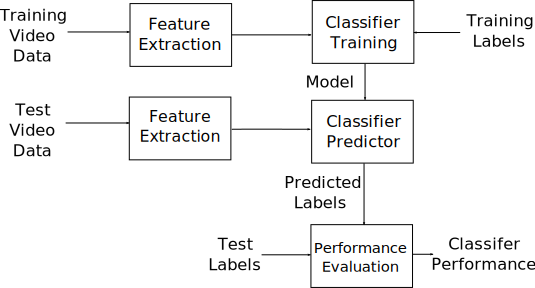
\includegraphics[width = 0.6 \columnwidth]{nvcclass/supervisedSystem.pdf}
\caption{Supervised learning uses labelled training data to create a model that can make label predictions for unseen data.}
\label{FigureSupervisedClassification}
\end{figure}

One of the aims of this thesis is to create an effective automatic system for \ac{NVC} recognition. After feature extraction and processing, the final step in an automatic system is often classification, which is the process of automatic prediction of a label based on a test sample observation. Many different classifiers have been applied to emotion, speech reading and gesture problems. This section provides an overview of the significant existing approaches to classification.

A supervised classifier is used to create a model based on labelled training data. This model can be used to predict labels for unseen test samples. The samples' features are usually the result of a \featureGeneration process from raw observations such as video frames. In this case, a test or training sample is a video clip of one or more frames. Given a set of training and test data, the performance of a classifier can be evaluated by comparing its predictions for unseen samples to the test data labels, also known as ``ground truth''. An illustration of this process is shown in Figure \ref{FigureSupervisedClassification}. There is a vast number of classification techniques in the published literature. Specific disciplines often have a set of preferred techniques that have been found to be effective. This is because each classifier has different requirements and makes different assumptions about the problem's characteristics. Also, each \featureGeneration technique has different properties, so features vary in suitability based on the problem and the specific classifier used. Rosenblum suggested that expressions with greater motion are easier to classify \cite{Rosenblum1996}. This section will focus on the use of classifiers in various facial classification applications and will discuss some of the classifier's properties in each context.

There are a few major families of classifiers, each requiring different formats for the input features and input labels. 
%The most common type of classifier have a single vector as an input feature, and a single discrete value as a label (and this is often restricted to a two class problem). Sequence classifiers, in contrast, have an ordered set of vectors to encode a sample's features. Multiple instance classifiers are similar to sequence classifiers but relax the ordering requirement for the sample's features. Classifiers also vary in that some require the feature vectors to use discrete values and others do not. 
For this reason, it is not possible to apply every classification technique to every problem. 
%Regression techniques are similar to classification techniques but use real values for their data labels. Regression is discussed further in Chapter \ref{ChapterNvcRegression}. 
The main families of classification techniques will now be discussed, along with the problems to which they have been applied.

\subsection{Single Instance Classifiers}

Single instance classifiers operate on samples that are represented by a single feature vector and a label value. This reliance on a fixed length feature vector makes classification of variable length clips problematic, but this can be overcome by \featureGeneration or decision level fusion. An early classifier was based on finding the $k$ nearest neighbours for a test sample \cite{Cover1967}. This approach is conceptually simple but it has high computer memory requirements. It also considers all feature components as equally significant, which can be problematic if some of the components of the feature vector are irrelevant. This may be the case for \ac{NVC} and emotion recognition, because typically only part of the face is relevant in determining the label. Donato \etal \cite{Donato1999} applied the nearest neighbour technique to facial expression classification. Nearest neighbour is appropriate for problems that have a large quantity of training data. Most classification techniques use a statistical model to approximate the decision boundary between different classes in feature space. One of the earliest classification techniques is \ac{FLD}, which attempts to use a linear manifold to separate two classes. Linear discrimination was applied to facial expression by Rose \cite{Rose2006}. 
%The boundary hyperplane can be specified by two points in feature space that are on opposite sides of the manifold and are equidistant from each point on the manifold. For facial features, these feature points corresponds to two exemplar face configurations; one exemplar corresponds to the positive class and one for the negative class. Hong \etal \cite{Hong2006} applied the enhanced Fisher linear discriminant model, which combines \ac{PCA} dimensionality reduction with \ac{FLD} to emotion classification. \ac{LDA} assigns class labels based on a test sample based on their proximity to each of the two samples. Based on this concept, we can see \ac{LDA} simplifies a complex nearest neighbour partitioning of feature space to a very simple partitioning. 
Unfortunately many problems in facial analysis require the use of non-linear decision boundaries to achieve acceptable performance.

\thesiscomment{DISCUSS \cite{Wang2006} using LDA for emotion?}
\thesiscomment{DISCUSS which methods are robust to outliers?}

A neural network is a machine learning technique based on an interconnected group of artificial neurons. Neural networks have high training requirements, and high computational and memory requirements. They also generate an internal model that is hard for humans to interpret and therefore only provide limited scientific insight. Their partitioning of feature space is also hard to grasp intuitively. However, neural networks have been used in a wide range of applications including speech reading \cite{Visser1999, Seguier2002}, emotion recognition \cite{Rosenblum1996, Petridis2009, Wollmer2009}, classifying laughter or no laughter \cite{Petridis2010} and many other non-facial analysis applications.

Boosting classifiers are a family of machine learning techniques that combine a set of weak learners into a single strong classifier. This is usually done iteratively and greedily, with weak learners being weighted and added to a bank of weighted weak learners. Many boosting approaches limited the weak learners to produce Boolean feature vectors and also require Boolean class labels. This makes some boosting methods less attractive if facial deformation features and \ac{NVC} labels can be considered as continuous values. One popular boosting method is Adaboost \cite{Freund1996}, which is a binary classifier known to be sensitive to outliers \cite{Natsuki2008}. Adaboost was applied to emotion classification by Moore and Bowden \cite{Moore07} and He \etal \cite{He2005}. Adaboost has been extended to temporal sequences and this is discussed in the later section on temporal model classifiers. The technical details of Adaboost are discussed in more depth in Section \ref{SectionAdaboost}. Boosting methods often explicitly select a subset of features which is easy to interpret and this can be useful in finding the types of face deformations that are responsible for determining the label of a test sample.

%Omitting Probabilistic Boosting-Tree? \cite{Tu2005} did someone use it? Adaboost was extended to multiclass \cite{Zhu2006}

A \acf{SVM} is a kernel based learning technique that attempts to learn a decision boundary that provides the maximal separation between positive and negative samples (Vapnick \cite{Vapnik1998}). In the input feature space, the boundary is non-linear and allows many complex problems to be addressed but at the risk of over-fitting, resulting in lower performance. The boundary model is based on adding weighted kernels centred at particular training samples. A test sample's distance from the boundary provides a mapping to a SVM space in which the problem is linearly separable. \ac{SVM} was originally formulated for binary classification and have since been extended in various ways, including for regression, which is used later in Chapter \ref{ChapterNvcRegression}.
%The original formulation was based on the two class problem, but various extensions for multi-class \ac{SVM} have been proposed and a compared between them was conducted by Duan and Sathiya Keerthi \cite{Duan2005}.
The \ac{SVM} method is popular and has been applied to facial analysis many times. It has been shown to be effective in emotion classification \cite{Goecke2006, Datcu2007, Seppi2008, Moore2009, Truong2009, Tariq2011, Jeni2011, Yang2011}, classifying pain or no pain \cite{Ashraf2007} and on \ac{AU} based expression recognition \cite{Taheri2011, Girard2011}. However, \ac{SVM}s do not provide an intuitive way to interpret their internal model, or to easily determine which features are most relevant. The technical details of the \ac{SVM} is discussed in more depth in Section \ref{SectionSupportVectorMachines}. A \acf{RVM} is a kernel technique that is closely related to \ac{SVM} but uses \ac{EM} to find a model to provide probabilistic label prediction. However \ac{EM} does not necessarily find a globally optimal model but still is an effective classifier that results in a sparser model and is often seen to result in a higher performance when compared to \ac{SVM} \cite{Nicolaou2011b, Xiangmin2007}. \ac{RVM} was applied to classifying brow action samples as posed or spontaneous by Valstar \etal \cite{Valstar2006}. \acf{SVDD} is another kernel method but in this case addresses the problem of modelling a single class's distribution. This was used by Zeng \etal \cite{Zeng2006} to model samples in one class labelled as ``emotional'' and this was used to classify test samples as either emotional or unemotional. This one class approach is useful if it avoids the problem of attempting to model a class which has a  complex feature space occupancy.

\thesiscomment{CHECK what does it mean when RVM is probabilistic?}

A decision tree classifier learns a graph of simple rules that recursively divide the feature space along axis parallel planes \cite{Breiman1984}. Decision trees are fast to train and apply, they provide a simple way for human inspection of the internal model and allow feature relevance to be determined. Decision trees were applied by Hillard and Ostendorf \cite{Hillard03} to agreement and disagreement classification in audio. Decision trees have been extended to random forests \cite{Breiman2001} in an attempt to improve performance. Random forests use an ensemble of decision trees with each tree trained on a different subset of features, using the concept of bagging. Random forests produce a verbose model that is difficult to interpret, in comparison to decision trees, but relevant features can still be evaluated. Random forests have been applied to emotion classification on posed data \cite{Fanelli2010}.

\thesiscomment{DISCUSS? Linear programming on emotion recognition \cite{Feng2005}, Dynamic Cascades with Bidirectional Bootstrapping on FACS \cite{Zhu2009}, Pair-wise machines on emotion \cite{SobolShikler2010}}

While some approaches to facial analysis have used human designed \featureGeneration, it is uncommon to attempt to manually create a classification model. However manual classification rules were created by Pantic and Patras \cite{Pantic2006} to classify \ac{AU} based facial expression. This allows human technical and intuitive abilities to be applied to the task to produce a tailored model, but this might not be appropriate for complex feature space distributions or in cases where the relevant features are unknown.

The classifier methods in this section have been concerned with samples having a single feature vector. The following section considers classifiers that specialise in modelling temporal and sequential problems.

\subsection{Temporal, Model Level Classifiers}

Temporal model classifiers are trained on samples that have been encoded as features that are an set of vectors. An ordered sequence of vectors is often based on sequential audio features, video frames or gestures in a clip of limited duration. This discussion will focus primarily on video classification, which is the topic of this thesis. Sequential temporal model classifiers attempt to model the temporal variation of features for each class. This model can then be used to predict a label for test samples. The most popular sequential classifier is the \acf{HMM}, which assumes a process can be characterised by transitions in a hidden state model. The transitions between hidden states are assumed to have a Markov property, which means the transition to the next state depends on the current hidden state but does not depend on previous hidden states. Each hidden state is associated with an emission model, which maps a hidden state onto a distribution of observable states. A separate \ac{HMM} is trained for each class, including a class specific hidden state transition model and an emission model. For gesture recognition, the hidden states are usually discrete labels, and the emission model is typically a Gaussian distribution. If features that encode facial expressions are used, each hidden state corresponds with a distribution of facial expressions. A particular class would be characterised by the transitions from one distribution of facial expressions to the next. 

\ac{HMM} is an elegant theory which has been successfully used in many applications. However, there are a number of disadvantages arising from model used and assumptions that are made. The hidden state model usually allows for self transitions to remain in a state. Because of the Markov property, the probability of remaining in one state reduces exponentially in time, and it is difficult to say if this would be appropriate for \ac{NVC}, or not. The emission model is assumed to be a Gaussian distribution which, for facial features, makes certain assumptions as to the properties of facial expression. Many of these issues can be addressed by increasing the number of hidden states in the model, but this quickly increases the number of unknown parameters in the transition model and the emission model. \ac{HMM}s typically operate best when there is a large quantity of training data available. The number of hidden states and the topology of the transitions are difficult to determine without manual adjustment, which makes the application of \ac{HMM}s rather time consuming and heuristic. Also, \ac{HMM}s use discrete class specific models and these cannot directly be used to predict continuous value labels.

\ac{HMM}s have been successful in the other form of human communication: verbal language recognition. Speech recognition often considers only the audible component but some studies have combined audio and visual facial analysis with \ac{HMM}s to improve recognition \cite{Potamianos2001, Nefian2002}. Language recognition can even be attempted with visual only features, although previous studies have been restricted to a limited grammar \cite{Luettin1996, Gray1997, Matthews1998, Saitoh2005}. Another quasi-verbal mode of human communication is sign language, to which a \ac{HMM} classifier has also been applied \cite{Starner1995}. Although almost entirely visual, sign language is generally not regarded as \ac{NVC} because multiple gestures are combined to form complex meanings. The difference between sign language and \ac{NVC} is that sign language has a grammar while \ac{NVC} does not. Emotion is also thought not to have a grammatical structure \cite{Cohen2000}. This lack of grammar makes it unlikely that \ac{HMM}s will be particularly effective for \ac{NVC} recognition. On more constrained problems, such as posed emotion or posed facial expression that begins and ends on neutral expression, a clear pattern of expression onset (appearance), peak and offset (disappearance) \cite{Ekman1984} can be seen. This may serve as a grammar of sorts, which can be used by a \ac{HMM} in facial expression classification \cite{Lien1998a} or emotion classification \cite{Cohen2000, Mower2009}. However, naturalistic emotion and \ac{NVC} does not necessarily begin and end with neutral expression and this reduces the consistency on which sequential temporal model classifiers depend. el Kaliouby and Robinson \cite{Kaliouby2005} use \ac{DBN}s, which are a generalisation of \ac{HMM}s to classifying mental states. Their approach integrates modelling of different temporal and spatial scales into a single classifier.

\thesiscomment{HMM on identity from lip shapes \cite{Mok2004}}

Adaboost was extended to consider temporal sequences as the TemporalBoost classifier and was tested on facial gestures by Smith \etal \cite{Smith2005}. This technique considers frames in a window of variable length, ending with the last frame of the sample. For each boosting iteration, the binary input features in the variable window have a logical ``AND'' and ``OR'' operator calculated, which are the values used for boosting. The variable window size is optimised to minimise the prediction error by gradient descent. As with most boosting methods, the trained model provides informative feature relevance information. Although this classifier considers multiple frames, it does not model how features vary in time in any direct sense. In testing, the order of frames in the window is not considered. Also the classifier is limited in that consecutive frames in a window must be considered, and the window end must correspond to the end of the clip, which makes it inappropriate if significant events occur at the start of a clip. As with Adaboost, TemporalBoost is limited to binary inputs and binary labels which makes it less relevant to continuous value problems.

A \acf{CRF} is a class of machine learning tools that, unlike conventional classification, which considers test samples independently, the label assignment of each sample considers the labels of ``nearby'' samples, which when applied to temporal data corresponds to nearby in time. In classification of video, this can enable a video frame to be classified based on adjacent frame labels. Hidden \ac{CRF} extends this with the addition of a latent, unobserved state. This method, like a \ac{HMM}, has discrete state transitions that are usually considered over short time periods. This may not be suitable for gradually varying human emotion and \ac{NVC} signals. Morency used \ac{CRF} to predict and recognise the behaviour of a human listener \cite{Morency2011}. Bousmalis \etal \cite{Bousmalis2011} used \ac{HCRF} to classify agreement and disagreement in political debates. This was later extended to \ac{iHCRF} \cite{Bousmalis2012}, which is capable of automatically finding the optimal number of hidden states. Rudovic \etal \cite{Rudovic2012} extended the \ac{CRF}-like \ac{CORF} method \cite{Kim2010} to take account of the ordinal relations between onset, apex and offset for \ac{AU} recognition. 

\thesiscomment{DISCUSS that we are classifying clips with a single label, rather than continuously varying sequences?}

Sequential classifiers consider samples that contain a set of ordered video frames. However, the following section will consider classifiers that specialise in classification of unordered sets, which may be appropriate for ``grammar free'' \ac{NVC}.

\subsection{Multiple Instance and Trajectory Classifiers}

\acf{MIL} considers classification of a set or ``bag'' containing one or more vectors or ``instances'' \cite{Maron1998}. This may be applicable to \ac{NVC} recognition, because it is possible that the presence of a single face configuration to be important in determination of the predicted label. If a particular area of feature space is critical to determine the label, it is known as a ``concept'', which corresponds to a specific face configuration. However, \ac{MIL} places minimal constraints or assumptions on the nature of the data, so there is no common \ac{MIL} approach. There are rather many different \ac{MIL} algorithms that have been proposed for domain specific problems. Also, it is unclear whether a single exemplar or concept is sufficient to encompass a range of naturally occurring \ac{NVC} signals. Tax \etal \cite{Tax2011} applied \ac{MIL} to emotion to find concepts that correspond to each class and applied the concept model to emotion classification. The face configurations corresponding to these concepts were not shown in the paper.

%Orther MIL approaches \cite{Wang2000}, \cite{Amar2001}, \cite{Zhang2001}, \cite{Andrews2003}, \cite{Goldman2003} \cite{Auer2004} \cite{Hiransoog2006}, \cite{Viola2007}, \cite{Leistner2010}

Time varying facial expression can be represented as a trajectory in feature space. Instead of attempting to model a class's trajectories' temporal pattern, Akak{\i}n and Sankur \cite{Akakin2011} directly compared trajectories using a modified nearest neighbour approach. The mean and median distance from a test trajectory to a class's trajectories was summed to produce a similarity score. As with conventional nearest neighbour classification, this method can be sensitive to irrelevant features, so this approach may benefit from feature selection.

The discussion so far has focused on papers that apply a classification method to facial analysis. The next section discusses papers that compare different classification methods for a specific application.

\subsection{Published Comparisons of Classifier Methods}

Various classification methods have been discussed, as well as their properties with respect to facial analysis and \ac{NVC}. However, it is difficult to discuss their relative performance without studies that directly compare classifiers on the same task. The best classifier for a problem is task specific, so these comparisons on emotion recognition provide circumstantial evidence that certain classifiers will be effective for \ac{NVC} recognition. However, this expectation is only by analogy and needs to be confirmed experimentally. Emotion and \ac{NVC} recognition are often interrelated but they are distinct problems.%, as discussed in Section \ref{}.
 
Sun \etal \cite{Sun2004} compared many classifiers for emotion recognition based on shape based, model fitting feature extraction. Their comparison included various Bayesian classifiers, variants of decision trees, \ac{kNN}, \ac{SVM}, etc. The authors were surprised that k-nearest neighbour classifier was most effective for this task. This suggests that the decision boundary between emotion classes is non-linear. Bagging and boosting, as an additional measure, was found to be beneficial to statistical model based classifiers. The large quantity of training data available for this application also makes \ac{kNN} more suitable in this case. Shan \etal \cite{Shan2009} used various classifiers for emotion recognition based on appearance based \ac{LBP} and Gabor features. The classifiers used were nearest neighbour, \ac{SVM} and Adaboost. In this case, \ac{SVM} was the most effective method, with nearest neighbour being the worse in performance. As well as providing another example of how different classifiers are effective for different tasks, the authors stress that effective \featureGeneration is critical to achieving good performance. Various \ac{SVM} kernels were compared and the \ac{RBF} kernel was found to have the best performance and generalisation. W\"{o}llmer \etal \cite{Wollmer2008} used audio features to classify emotional activation and valence. \ac{CRF} performance exceeded \ac{SVM} performance for classification. However, a regression approach to this task may be more appropriate than the use of classification.

Other comparisons of classifiers for facial analysis have been conducted that do not use emotion labels. Petridis \etal \cite{Petridis2009} compares static and temporal model classifiers for smile classification based on shape features. When considering frame based features, there was no significant difference between sequential and non-sequential classifiers. For window based features, static classification exceeds the performance of sequential classification. This suggests that \featureGeneration that encodes temporal information is more important than temporal modelling by a classifier for this task. Escalera \etal \cite{Escalera2009} used appearance and detection based features on conversation dominance labelled data. The compared classifiers were Discrete Adaboost and \ac{SVM} (with \ac{RBF} and linear kernels) with Adaboost having the best performance and generalisation. Tax \etal \cite{Tax2011} used tracking based features to classify facial expression. Several classifiers were used including \ac{LDA}, diverse density \cite{Maron1998} (a \ac{MIL} method), a \ac{MIL} clustering based method, \ac{HMM} and \ac{CRF}. The performance for several different \ac{AU}s is shown but there is no single classifier that is optimal for all.  In some cases a sequential classifier is useful, sometimes a \ac{MIL} classifier is optimal and in other cases, a non-sequential classifier is best. A similar mixed result of performances was found by Akak{\i}n and Sankur \cite{Akakin2011} in use of various features to recognise head gestures. Their results are discussed in more depth in Section \ref{SectionHmm}, because their paper is partly a response to results in Chapter \ref{ChapterClassification}. There was no clear winner between sequential and \ac{MIL}-like approaches. However, they found that better performance could be gained by decision level fusion of different classifiers. Pfister \etal \cite{Pfister2011, Pfister2011b} used a temporal appearance based feature to attempt to classify masked emotion from microexpressions. In this study, \ac{MKL} provided a performance advantage over \ac{SVM} in classifying emotion into present or not-present. However, random forests were best at detecting the presence of micro-expressions from a background of neutral expression. The experimental conditions of this study were different from natural social situations, so it is hard to draw firm conclusions on the best approach to \ac{NVC} recognition. Rose \cite{Rose2006} compared multi-class classification to single class recognisers for expression recognition and found that linear discrimination and kernel based multiclass classifiers was most effective. Rudovic \etal \cite{Rudovic2010} compared \ac{RVM}s, \ac{SVM}s, linear regression and Gaussian Process Regression on the CMU Multi-PIE facial expression database and found that \ac{RVM}s combined with pose normalisation was most effective. Buciu \etal \cite{Buciu2009} compared the cosine similarity matrix with \ac{SVM}s for expression recognition, based on various \ac{ICA} approaches. They found that different \ac{ICA} methods reduced mutual energy in basis images, which was negatively correlated with recognition performance.

\section{Conclusion}

There are a few conclusions that can drawn from the literature. There is no single approach, be it a \featureGeneration method, temporal analysis method or classifier that is suitable for all problems. There are certainly differences in popularity of classifiers, with \ac{HMM} and \ac{SVM} being dominant in facial analysis, while decision tree based methods are relatively rare. It is also frequently observed that for a set of behaviours, a subset is easier to automatically recognise than others. The next chapter describes the collection of a corpus of informal conversations that is suitable for training an automatic system.

\thesiscomment{DISCUSS feature and decision level fusion, decision: \cite{Kittler2003}, \cite{Lucey2009}, \cite{Pfister2011b}, fusion: \cite{Kanluan2008}, \cite{Petridis2008}, \cite{Petridis2009}}


%
\def\meshpos{\textbf{p}}
\def\templatepos{\textbf{a}}

\chapter[Online Tracking]{Online Tracking}
\label{ChapterOnlineTracking}

\section{Introduction}

\section{Related Research}

\subsection{Boston Head Pose Corpus}

\section{Description of System}

\subsection{Initialisation}

\subsection{Head Pose Estimation by LM}
\label{SectionLmHeadPose}

Original idea: \cite{Liu2000}

\begin{equation}
\mathcal{F}(\textbf{R},\textbf{t}) = \displaystyle\sum_{i=1}^{\numFeatures} { ||\textbf{\templatepos}_{i} - proj(\textbf{R} \textbf{\meshpos}_i + \textbf{t})||^2 }
\label {LmPoseEquation}
\end{equation}

\subsection{Online Learning}

\subsection{Tracking with Multiple Templates}

\subsection{Estimate pose using Weighted RANSAC LM}

\subsection{Update tracker positions}

\section{Experimental Results}

\subsection{Head Pose Estimation}

\subsection{Facial Feature Tracking on Boston}

\subsection{Facial Feature Tracking on TwoTalk?}

\thesiscomment{Do we need to do these experiments?}

\section{Discussion}

\thesisstatement{Some features accurately track over a wider pose range than others}

\thesisstatement{Banks of pose specific head trackers can be used to extend the pose range that can be accurately tracked.}

\thesisstatement{The proposed online learning system can track faces accurately over a wide range of poses for smooth head motion.}

\thesisstatement{Poor initialisation of head pose in the online tracking system, often caused by difference face shapes, causes poor performance throughout the video.}

\thesisstatement{Online tracking system works on smooth motion sequences (Boston) but fails on unconstrained video.}

Why we don't use online tracking system later in the thesis?

\thesisstatement{LP Flocks are better than Online Tracker for TwoTalk videos.}


\section{Conclusions}

DISCUSS: Say how this is still an unsolved problem and neither this nor LPs fully address it


\begin{savequote}
Verbal and nonverbal activity is a unified whole, and theory and methodology should be organized or created to treat it as such.
\qauthor{Kenneth L. Pike}
\end{savequote}

\chapter[The LILiR TwoTalk Corpus and Annotation Data]{The LILiR TwoTalk Corpus and Annotation Data}
\label{ChapterCorpus}

\thesiscomment{MAIN POINT: Because NVC is dependent on social situation and no appropriate database is available, we record and annotate a new NVC database that has minimum experimental constraints and annotated using high dimensional labels.}

\thesiscomment{WHAT we do}

\thesiscomment{HOW we do it}

\thesiscomment{RESULTS, IMPACT and NOVELTY}

\ac{NVC} occurs as a component of almost all forms of human communication. In order to study it, it is usually convenient to record a representative sample of human communication for later analysis. This set of data is called a ``corpus''. The observations in the corpus are usually labelled by a group of observers or annotators. 
%Annotations are used to systematise the content in the corpus to facilitate further analysis. 
The manner of recording and the type of annotation is dependent on the behaviour under investigation. This chapter describes the collection of a new corpus that occurs during informal conversations. Minimal experimental constraints are used in order to retain the natural and spontaneous characteristics of informal conversation. %However, the recorded sessions were conducted in a studio environment between pairs of selected participants, which may differ from informal conversations in the field.

The corpus described in this chapter has been named the LILiR TwoTalk corpus\footnote{The name derives from this work being associated with the EPSRC LILiR project.}. 
%At the time of recording, there were no similar publicly available \ac{NVC} data sets that were naturalistic (non-role play or otherwise contrived by the experimenter), suitable for tracking and spontaneous\footnote{This is discussed further in Section \ref{SectionExistingDataSets}}. 
At the time this work was conducted, there were limited appropriate data sets that were publicly available. Corpuses have been recorded in various situations with a range of spontaneity and naturalness. The most viable candidate was the AMI meeting corpus \cite{Carletta2007}. However, only a portion of this corpus is naturalistic and it was not suitable for the feature tracking method employed in Chapter \ref{ChapterClassification} and subsequent chapters. This chapter describes a new corpus that was designed specifically to fit the requirements of this study.

Posed data differs from spontaneous data in many ways because \ac{NVC} signals are dependent on social context\footnote{Even if posed data is considered as having no social context, the absence of a social context is a factor in \ac{NVC} expression.}. Informal conversations can be recognised in other cultures because they have some characteristics that are cross-cultural. The choice of a common, reproducible social situation is attractive for cross cultural study. The social situation of informal conversation is easy to organise and reproduce experimentally. However, spontaneous data is challenging to annotate because of the \ac{NVC} signals being sparsely distributed throughout lengthy videos. Also, there is no clear application for informal conversation behaviour recognition at this time apart from further improving our understanding of human behaviour.
%This corpus is used in later chapters of this thesis for training an automatic system. 
Previous annotation approaches have focused on encoding a subject's internal state, emotions, gestures, dialogue acts, social relationships, topic, attention or expressions. The LILiR TwoTalk corpus uses annotation labels that encode the communicative non-verbal behaviour \cite{Ekman1969}, including both the verbal and \ac{NVC} aspects. 
%The labels of overall meaning provide a basis for an investigation into the association between \ac{NVC} gestures and communication meaning.

The main contributions of this chapter are:

\begin{itemize}
 \item a new corpus of informal conversations between pairs of people which is suitable for the study of \ac{NVC} signals,
 \item an annotation set of communicative non-verbal behaviours. The annotation was performed using a new set of \ac{NVC} quantised, dimensional labels,
 \item inter-annotator agreement of the collected data was analysed and 
 \item co-occurrence of \ac{NVC} signals was found and
 \item the recordings and annotation data are publicly
 available\footnote{\scriptsize{http://www.ee.surrey.ac.uk/Projects/LILiR/twotalk\_corpus/}}.
\end{itemize}

The next section provides an overview of recording conditions, annotation systems and related work. The recording of the new corpus is described in Section \ref{SectionDataCapture}. Section \ref{SectionDescribeQuestions} describes the questionnaire used by the annotators. Section \ref{SectionMultiCultitureAnnotation} describes how multiple annotators rated the corpus video samples. Demographics of the annotators are described in Section \ref{SectionAnalysisOfHumanAnnotation} and Section \ref{SectionAnalysisOfMeanRatings} investigates patterns occurring in the annotation data.

\section{Related Research}
\label{BackgroundCorpus}

This section describes the creation and use of corpuses that can be used as the basis for computer based analysis. The most significant social situations and annotation systems are discussed, as well as the existing data sets. %The situation in which a corpus is recorded, if used to train an automatic recognition system, determines in which situations the system may be deployed effectively.

%An early use of video recording to study \ac{NVC} was performed by Condon and Ogston \cite{Condon1971} in which the material was replayed slowly to allow better manual observation. More recently, the use of computers enables some types of human behaviour to be analysed automatically, and patterns can be found that are difficult for humans to manually identify.

%Practical guidance on recording \cite{Frank2005}
%High level look at factors in designing human databases \cite{Cowie2008}
%Emotaboo design considerations \cite{Zara2007}, also EmoTV \cite{Devillers2008}, \cite{Afzal2009}, FreeTalk \cite{Campbell2010}, B3D(AC)\^2 \cite{Fanelli2010b}, D64 \cite{Oertel2010}

\subsection{Social Context}
\label{BackgroundSocialContextUsedInTwoTalk}

%Context is important for literal meaning too \cite{McHoul08}
% Review of data sets, etc \cite{Cowie2005}
%Other acted data set use \cite{Smith2005}, \cite{SobolShikler2010}, FERA \cite{Tariq2011}, movie extracts \cite{Kipp2009}
%Meeting, AMI corpus , \cite{Hillard03}, \cite{Petridis2010}, \cite{Truong2009}
%Interview \cite{Grimm2007}, \cite{Kanluan2008}, \cite{Devillers2008}

Acted corpuses are convenient to use because the samples have a predetermined ground truth and little recording time is wasted on uninteresting behaviour. It is impossible to predict or control the specific behaviours that will occur in naturalistic behaviour, and therefore videos require annotation to determine the labels. The sections of the video that are of interest to researchers may be unevenly distributed. Contrived situations, such as role play, tasks and games are an intermediate approach, in which participants are guided by the experimenter to maximise the useful content and allow for natural reactions to unnatural stimuli. As discussed in Section \ref{BackgroundWhatFactorsInfluenceNvc}, the situation in which a corpus is recorded affects the behaviours that occur. 
%The type of situation in which a corpus is recorded should be driven by the intended application of the final system. 
%This section will review some of the common contexts used for recording corpus data, and some background on the informal conversational context.

Historically, a large amount of emotion recognition research has been conducted on acted data sets, in which participants are told to express or pose particular behaviours, or the behaviour is expressed in a contrived or rare social situation. Often, a sequence starts and ends with a neutral expression. However, spontaneous emotion can change without transitioning through a neutral expression. Novel methods continue to be proposed for acted data sets \cite{Chew2012b}, including: {BU-3DFE} \cite{Moore2009}, {JAFFE} \cite{He2005}, Mind Reading {DVD} \cite{Kaliouby2005} \cite{SobolShikler2010} and {GEMEP}-{FERA} \cite{Valstar2011}. Emotion recognition based on basic emotions is generally considered a solved problem \cite{Valstar2012}. Many studies are based on elicited emotional responses from subjects that are interacting with a device being controlled by the experimenter \cite{Afzal2009}, e.g. viewing videos \cite{Sun2004, Pfister2011}, interacting with computer characters (e.g. SAL) \cite{Wollmer2009} or a robot \cite{Seppi2008}. This method is also referred to as a ``Wizard of Oz'' situation. Further naturalism is added by having a social situation with two or more humans participating in a task. Data can be recorded in a game environment, such as EmoTaboo \cite{Zara2007}, interviews \cite{Cowie2009} or in a niche social situation, such as speed dating \cite{Madan2005}. Contrived social situations, in which participants spontaneously react to an experimenter designed social situation, include staged interviews \cite{Zeng2006} or meetings, such as in the majority of the AMI meeting corpus \cite{Carletta2007} for which approximately ''two-thirds of the data has been elicited using a [role-play] scenario'' \cite{amiproject}. Few studies consider social situations that are not contrived or goal based activities. Almost all studies occur in the laboratory, due to the practical difficulty of recording natural social situations. Controlled situations can be useful for data collection if the automatic system is intended to be deployed in such an environment. %Given the need for naturalistic data, it might be advantageous to select a common social situation, such as informal conversation, that contains rich and diverse \ac{NVC}.

Informal conversations are used throughout this thesis. An informal conversation is a common social situation and one which almost everyone experiences on a daily basis. This context is also referred to as ``casual conversation'' or as ``chatting''. These conversations are usually relaxed, unfocused discussions about trivial matters. Eggins and Slade \cite{Eggins1997} defines casual conversation as ``talk which is NOT motivated by any clear pragmatic purpose''. This social context has not received much attention from linguists or from the human behaviour recognition community. Humphrey claimed that casual chatting can be recognised across cultures because of the activity's characteristics \cite{Humphrey1993} which are:

\begin{itemize}
 \item being informal,
 \item lacking focus,
 \item containing haphazard reiteration and
 \item having ``topics of conversation crumble away in the compulsion of people saying what they can't help saying''.
\end{itemize}

Automatic recognition of \ac{NVC} in informal conversations is attractive for a number of reasons. Informal conversation is a specific social situation that is relatively easy to replicate (specifically, the social context can be staged relatively easily). It is also commonly occurring, cross cultural and occurs in almost all social groups.

However, there are potential drawbacks compared to other approaches:

\begin{itemize}
 \item the frequency of strong emotion and intense \ac{NVC} is relatively low,
 \item there are times in which the participants are passive, which contains little information of interest and
 \item labelling must be performed by annotators.
\end{itemize}

The annotation of the data is discussed in the next section.

\subsection{NVC Annotation, Questionnaire Design and Labels}
\label{BackgroundWhyNvcAnnotationIsBoring}
\label{BackgroundMultipleAnnotation}
\label{BackgroundQuestionaireDesign}

Annotation uses human observers to review and provide judgements regarding the content of the corpus. Video clips are viewed by each annotator and rated based on questions set by the experimenter. The purpose of annotation is to record the way the corpus is perceived by the annotators and thereby provide a basis to study the content of the corpus.

%NVC annotation difficult 

Many factors influence the perception of \ac{NVC} signals (see Section \ref{BackgroundWhatFactorsInfluenceNvcPerception}). For annotation of a corpus, these factors are still present but can be somewhat controlled. Studies have focused on the annotation perception issue, in an attempt to reduce inter-annotator disagreement and to improve the quality of the data. Reidsma claimed that inter-annotator agreement is caused by poorly chosen annotation concepts and annotation schema, clerical errors, lack of annotator training, as well as context \cite{Reidsma2008}. His thesis is currently the broadest review of the annotator agreement issue. Experts can be more consistent than untrained observers for some annotation tasks, e.g. high quality \ac{FACS} \cite{Donato1999}. Annotation can be improved by showing the video leading up to an emotion \cite{ElKaliouby03}, as well as showing them the entire corpus before starting to annotate \cite{Hoque2009}. Studies have noted that inter-annotator agreement was lower for stylised emotion than for spontaneous emotion \cite{Bernhardt07, Afzal2009b}. Annotation labels that require less interpretation might be thought of as advantageous because they have higher inter-annotator agreement \cite{Fasel2003}, but this avoids the problem of perceptual differences which needs to be addressed for effective \ac{NVC} recognition.

Annotation of emotion data sets have often been performed by multiple observers. The annotators use a task specific encoding system that is selected or designed by the experimenter. These annotations are usually combined to form a consensus score, either by taking the majority vote in the case of discrete classes \cite{Seppi2008, Escalera2009}, or taking the mean in the case of dimensional variables \cite{Wollmer2008, Mower2009}. In this case dimensional is defined as ``the range over which or the degree to which something extends'' \cite{merriamwebster}. This is done to reduce the effect of different interpretation among the annotators and emphasise the generally agreed content of the corpus. However, this attempt to minimise the role of interpretation differences makes the ground truth differ from the individual human observations. A less common approach is to consider subsets of annotators and model them individually. A subset of annotators that had inter-agreement was modelled by Reidsma and op den Akker \cite{Reidsma2008b}. Groups of annotators can be collected and handled separately, as in the case of naive and expert annotators \cite{Donato1999}. Although judgement based annotation is almost universally used, a few studies have used self assessment \cite{Madan2005} or a combination of self-assessment and annotator judgements \cite{Hoque2009}. 
%We have discussed how selection of corpus data and annotators is important for useful annotation data. 
%The choice of encoding schemes, including labels and discrete/continuous scales selection, will now be reviewed.

%The choice of annotation label used is important in determining the possible applications for the data. 
There are many pre-existing annotation systems that encode facial expression, emotion, mental states, affective state, gesture, dialogue acts, social relationships, attention and communication. These systems can be broadly grouped into four classes: those that assess the internal state of a person, a person's physical behaviour, social dynamics between people and those that describe the meaning of specific actions. Emotion labelling is one of the most popular facial or mental state labelling systems. The most common emotion labelling system is based on discrete classes, occasionally using the original Ekman 6 basic emotions \cite{Cohen2000}. There are no commonly agreed set of emotions and the choice of appropriate labels would depend on the intended application. Discrete emotional classes cannot comprehensively cover all emotional states and instead focus on episodic occurrences \cite{Cowie2005} while ignoring pervasive emotion. Pervasive emotions are emotional states that are routinely experienced in life but not present in an emotionless state. 

Emotion labelling has often been expressed in a dimensional, abstract 2{D} space such as activation and evaluation \cite{Cowie2000} or valence and activation \cite{Cowie1999, Liscombe2003, McRorie2007}. In this case, abstract means ``non-prototypical'' and ``defined in terms of natural language'' \cite{Kazemzadeh2013}. It is unclear how many dimensions are necessary to faithfully encode human perception of \ac{NVC} or emotion. A 2{D} space may not be enough to encode all emotions unambiguously \cite{Fontaine2007}. Schr\"{o}der \etal claimed that emotion could be effectively encoded using only 2 dimensions \cite{Cowie2000} in a system such as ``FeelTrace'', but they admit there was ambiguity in distinguishing between anger and fear. However, dimensional encoding is not limited to these labels: Ashraf \etal \cite{Ashraf2007} used a dimensional scale for rating pain, Mikels \etal \cite{Mikels2005} collected emotional annotation data for images using \textit{fear}, \textit{sadness}, \textit{disgust}, and \textit{anger}, each measured on independent, 7 point Likert scales and Ball and Breeze \cite{Ball2000} using dominance and friendliness dimensions to encode personality. Dimensional scales have also been used to rate toddler behaviour \cite{Lorber2003}, facial action intensities \cite{Fasel2000}, happiness and sadness \cite{Hsee1992}, classroom interactions\footnote{http://www.teachstone.org/about-the-class/} and non-verbal behaviour \cite{Feldman1991}. The diversity of labels used in dimensional systems is broad to cover the variety of scientific problems to be addressed.

The AMI corpus includes many types of annotation labels including dialogue acts, attention and specific gestures \cite{Carletta2007}. The annotation was later expanded with dominance \cite{Aran2010} and emotion. Devillers \cite{Devillers2008} used a different labelling system based on appraisal theory \cite{Scherer1999}, in which the emotion stimuli are rated rather than the mental state.

%Other emotion labelling examples  \cite{Dornaika2005} \cite{Abrilian2006} \cite{Hong2006} \cite{Wang2006} \cite{Zeng2006} \cite{Lee07} \cite{Datcu2007} \cite{Grimm2007} \cite{Moore07} \cite{Zara2007} \cite{Kanluan2008} \cite{Seppi2008} \cite{Moore2009} \cite{Mower2009} \cite{Fanelli2010b} \cite{SobolShikler2010} \cite{Tariq2011} \cite{Nicolaou2011}
%other Ekman based \cite{Feng2005}
%other abstract \cite{Cowie2000}, 

Various encoding systems have been discussed but the choice of the most appropriate system is dependent on the type of behaviour of interest to the experimenter. Annotation labels can focus on either the internal mental state or the intentional communication but not usually both. An example of labels that focus on internal states is the Mind Reading corpus, originally created to assist autistic observers to recognise a mental state in others. This was applied to automatic recognition by el Kaliouby and Robinson \cite{ElKaliouby2004} for a subset of labels: agreeing, concentrating, disagreeing, interested, thinking and unsure, with the emphasis on mental state. Afzal \etal used similar affect labels for recognition \cite{Afzal2009b}. Pain has also been used for annotated and automatic recognition \cite{Ashraf2007, Lucey2009}. 

Annotation labels which focus on verbal communication meaning can also be applied to \ac{NVC}. Hillard and Ostendorf \cite{Hillard03} performed classification using agreement and disagreement labels on intentional verbal utterances. Zara \etal \cite{Zara2007} used high level groupings of verbal communication acts in EmoTaboo, some of which correspond to a meaningful communication. Bavelas and Chovil \cite{Bavelas97} counted the frequency of meaningful facial gestures. 
%The other labelling systems that have been used for automatic system training have focused on mental states, expression or gesture.

Another group of human behaviours that are of interest to researchers is facial expression. Facial expressions are an externally observable movement of the body which require less interpretation than emotion to annotate. This is in contrast to emotions which largely occur in the mind and only sometimes manifest themselves in behaviour or expression. 
%A facial expression can be associated to an \ac{NVC} meaning or emotion but this association is dependent on context. 
The most popular method for encoding facial expression is the \acf{FACS} \cite{Ekman1978}, in which facial \acf{AU}s correspond to sets of muscles. \ac{FACS} is widely used for labelling expressions and has been used as the basis for regression systems (\cite{Savran2012}), although most papers only use a subset of \ac{FACS}. However, \ac{FACS} annotation exhaustively encodes expressions, requires trained observers and is very time consuming to perform. The encoding is typically based on binary classes and does not consider the intensity of expression. 
%This loss of information may be significant for some applications, such as lip reading. 
Others have used expression labels that did not use the \ac{FACS} system, for example Kanaujia \etal \cite{Kanaujia2006} labelled nodding and blinking.

%other FACS based labelling \cite{Bartlett2006} \cite{Tang2007} \cite{Zhu2009} \cite{Tax2011} \cite{Taheri2011} \cite{Girard2011} \cite{Jeni2011} \cite{Valstar2012}

There are other facial analysis labelling approaches that do not fit with the previously discussed groups but have some relation to \ac{NVC}. Deception and truthfulness modifies the perception of communication and have been used as labels and in recognition \cite{Tsiamyrtzis07, Pfister2011}. 
%Naturalistic deception is not an intentional action and is therefore not a communication act. 
The outcomes of speed dating was labelled and recognised \cite{Madan2003} and this again is largely based on perception of \ac{NVC}, but the labels themselves do not correspond to meaningful communication. 
%Labels-laughter \cite{Petridis2008} \cite{Petridis2009} \cite{Truong2009} \cite{Petridis2010}
%Labels-identity \cite{Mok2004} \cite{Fang2009}
%Labels-social-dynamic \cite{Escalera2009}
Given that the situation in which data is recorded is significant, the next section discusses why a new naturalistic data set is needed for studying occurrences of meaningful \ac{NVC} signals.

\subsection{The Need for a Naturalistic Corpus}
\label{BackgroundNeedNaturalistic}

\thesisstatement{Recording social situation while seated in the lab and with no constraints on conversation topic provides data useful for studying social interactions (compromise between spontaneous conversations and getting useful data).}

\thesisstatement{Literature suggests significant differences in posed vs. natural human interaction}

\thesisstatement{Classifying naturalistic data is harder than posed data \cite{Akakin2011}}

There has long been criticism of the study of social phenomena in a laboratory environment. Although a laboratory is intended to assist the control of experimental variables, Argyle \cite{Argyle1975} claimed that too often study subjects ``sit in cubicles by themselves, watch flashing lights and press buttons; often there is no verbal communication, no NVC, no real motivation, and there are no situational rules''. Moving a social situation from its normal location to the laboratory can have significant effects, due to the subject's knowledge that they are being recorded \cite{Beattie1982b} but ethical and practical considerations make this fact hard to conceal \cite{Frank2005}. Posed and spontaneous data also have significant differences. If meaning in communication is the subject of study, context is significant which makes posed or over simplified data unsuitable \cite{Bavelas97}. However, not all human related research needs to be naturalistic and researchers need to assess the suitability of any database \cite{DouglasCowie2003}. Many emotion recognition systems have used posed data and this seems unlikely to change. However, different recording conditions have been shown to result in different behaviours. If an automatic system is trained based on a corpus and deployed in a different environment, it is quite possible that human behaviours will be significantly different and the automatic system will have poor performance. For example, the timings of natural and posed emotions are different \cite{Cohn2004}. This difference is so significant that posed and spontaneous examples of emotions can be manually and automatically distinguished \cite{Valstar2006, Pfister2011b}. Strong emotion is rarely expressed or is expressed in unusual circumstances, making recording of naturalistic examples difficult \cite{Cowie2008}. For natural data, the information content is unevenly distributed in time \cite{Cowie2009}. Rapid emotional transitions are more common in natural data than in posed data \cite{McRorie2007, Bavelas97}. Rapidly changing emotion has higher annotation demands and less predictability in recognition. Cowie \cite{Cowie2008} reviewed these issues in the context of creating databases suitable for human behaviour and concluded the challenges for recording and annotating such a database are significant, but stressed that these issues must be addressed to make progress. An alternative to using naturalistic data as the basis for automatic systems is to use data ``of a kind that might have to be dealt with in an application'' \cite{Cowie2009b}. In recent research, these types of datasets are becoming more popular. It is likely that some applications of \ac{NVC} recognition require the use of naturalistic data and this remains the focus of this thesis. 
%Given the need for naturalistic data, the next section reviews the existing data sets, focusing on naturalistic corpuses.

\subsection{Existing Data Sets}
\label{SectionExistingDataSets}

The majority of facial analysis and human behaviour data sets have focused on emotion or expression recognition. As discussed in the previous section, there is a need to use natural data, therefore many of the existing data sets are not appropriate for \ac{NVC} recognition. The existing naturalistic, public databases will be reviewed and the reasons for recording a new data set will be discussed in this section.

\begin{itemize}
\item \textit{Belfast Naturalistic Emotional Database} is a corpus using both television programmes and interviews \cite{Cowie2005}. The clips are between 10 and 60 seconds in duration. The variability of social context would make expression of \ac{NVC} rather diverse. Also, some of the social situations are rare, such as being an interviewee on a television programme.
\item \textit{EmoTV} comprises of 89 television interview monologues. The duration of video clips varies between 4 and 43 seconds. Again, the variability of social context is an issue, as well as the low quality of analogue broadcast TV. \cite{Devillers2008}
\item \textit{FreeTalk} is a four person conversation which was not limited in topic. Participants remained seated throughout. The conversation was conducted in a laboratory. This corpus is similar to the one presented in this chapter but FreeTalk was publicised after the TwoTalk corpus was recorded and used \cite{Campbell2010}.
\item \textit{D64 Multimodal Conversational Corpus} used unrestricted, multi-person conversation in a domestic environment \cite{Oertel2010}. This corpus is a significant improvement on previous data sets in that it recorded casual conversation outside of the laboratory environment. The subjects could move around or leave as desired. This data set was also publicised after the corpus in this chapter was recorded and used.
\end{itemize}

Although not the primary focus of this thesis, existing non-naturalistic datasets include:

\begin{itemize}
\item \textit{Canal9} is a series of broadcast television political debates between 2 or more participants and a moderator. This corpus is discussed in more detail in Section \ref{SectionCanal9}.
\item The majority of the \textit{AMI Meeting corpus} is a series of recordings of role play meetings in a group of 4 people. Approximately two thirds of the meetings are role play scenarios, and the remainder are naturalistic. People occasionally moving from seated to standing (Figure \ref{FigureAmiMeetingStanding}).
\item \textit{EmoTaboo} is a set of recordings of role play games between two participants.
\item \textit{MMI} is a searchable database of posed and elicited emotions.
\item \textit{Mind Reading} corpus is a library of short, silent videos of mental states performed by actors. This was originally produced as training material management of autism spectrum disorders. This corpus is described in more detail in Section \ref{SectionMindReading}.
\item \textit{Sensitive Artificial Listener (SAL)} is a corpus of elicited emotion based on a human interacting with a computer character that exhibits one of a set of personality types.
\item \textit{Green Persuasive Dataset} is a series of recordings of a role play situation between an experimenter and a volunteer with the discussion topic focused on environmental issues. The experimenter attempts to persuade the volunteer to adopt a more environmentally sustainable lifestyle.
\item \textit{MHi-Mimicry-db\cite{Sun2011}} is a 15 camera, 3 microphone recording of dyadic conversations. The participants were either in a political debate (34 recordings) or in a role-playing game (20 recordings).
\end{itemize}

\begin{table}
\centering
\caption{Summary of data sets used for emotion and conversation oriented research.}
\tiny
\begin{minipage}{0.99 \columnwidth}
\begin{tabular}{ | c | c | c | c | c |}
\hline
Corpus & Duration & Context & Participants & Labels \\% & Availability \\
\hline
Belfast Naturalistic \cite{Cowie2005} & 86 min labelled & emotional & Dyadic & Emotion  \\%& Subset is public \\ %(Feeltrace)
& 12 min available & interview & & \\
\hline
EmoTV \cite{Devillers2008} & 89 clips, 12 minutes & interview monologues & Monologue & Various \\% & Proprietary \\
\hline
FreeTalk \cite{Campbell2010} & 270 minutes & lab, conversation & 4 person & Various \\% & Public \\
\hline
D64 Multimodal \cite{Oertel2010} & 8 hours & domestic, conversation & 4-5 people & Unknown \\% & ? \\
\hline
Canal9 \cite{Vinciarelli2009}& 42 hours & debate & 2 to 4 person & Shots, ID \\% & Public\\
& & & \& moderator & \\
\hline
AMI Meeting \cite{Carletta2007}& 100 hours & Role play meeting& 4 people & Various \\% & Public, hi quality video on DVD\\
\hline
EmoTaboo \cite{Zara2007}& 8 hours & Mime game & Dyadic & Emotional Events\cite{Devillers2008} \\%& By arrangement\\
\hline
MMI \cite{Valstar2010}& Increasing with time & Various induced & Single participant & Various \\% & Public\\
\hline
Mind Reading\footnote{http://www.jkp.com/mindreading/} & \textasciitilde19 minutes & Posed & 1 Actor & Mental state \\% & Commercial\\
\hline
SAL \cite{Schroder2011}\footnote{http://semaine-db.eu/}& \textasciitilde10 hours & Wizard-of-OZ & 1 person & Emotion \\% & Available on CD\\ %(Feeltrace)
& & & with computer & \\
\hline
Green Persuasive& videos 25-48 minutes & role-play & dyadic & persuasiveness \\% & Public\\
Dataset\footnote{http://green-persuasive-db.sspnet.eu/} & 8 dyads & & & \\
\hline
MHi-Mimicry-db\cite{Sun2011} & \textasciitilde12 hours & discussion/role play & 40 people, dyadic & various \\
\hline
\end{tabular}
\end{minipage}
\normalsize
\label{TableAvailableDatasets}
\end{table}

\begin{table}
\centering
\caption{Summary of adverse factors for the suitability of existing datasets.}
\tiny
\begin{minipage}{0.99 \columnwidth}
\begin{tabular}{ | c | l |}
\hline
Corpus & Suitability \\
\hline
Belfast Naturalistic \cite{Cowie2005} & Staged interview, only a \textasciitilde12 min subset is available \\
& not labelled for \ac{NVC}, face size is small (approximately 150 by 200 pixels) \\
\hline
EmoTV \cite{Devillers2008} & Not publicly available \\
\hline
FreeTalk \cite{Campbell2010} & Video is small and faces are approximately 18 by 18 pixels \\
& unsuitable for tracking, only publicly available recently (since 2010) \\
\hline
D64 Multimodal \cite{Oertel2010} & not publicly available at time of writing \\
\hline
Canal9 \cite{Vinciarelli2009}& Unusual social situation, only a subset is annotated \textasciitilde10 min \\
 & not continuous view of subject, low quality interlaced broadcast video,\\
 & standing multiple participants may result in larger head pose changes \\
\hline
AMI Meeting \cite{Carletta2007}& Mostly contrived role play scenario \\
& although some meetings are naturalistic, \\
& not \ac{NVC} annotated, emotion annotations are not publicly available \\
& multiple participants may result in larger head pose changes \\
& and more complex interactions, video is highly compressed, \\
& face size is small (typically 110 by 70 pixels), \\
& contains a mixture of standing and seated behaviour \\
\hline
EmoTaboo \cite{Zara2007}& Not publicly available \\
\hline
MMI \cite{Valstar2010}& Focused on posed and induced expression not \ac{NVC} \\
& Only uses a single participant and not dyadic\\
\hline
Mind Reading& Acted, low quality video, face only 100 by 150 pixels, focuses on mental states not \ac{NVC} \\
\hline
SAL \cite{Schroder2011}& Human to computer character conversation rather than human to human conversation \\
& Available since Mar 2009 \\
% \hline
\hline
Green Persuasive& Contrived social situation, available since 2009, \\
Dataset & Small videos with face approximately 104 by 145 pixels\\
\hline
MHi-Mimicry-db\cite{Sun2011} & staged discussions or role-playing games, \\
& labelled for facial expression not \ac{NVC}, only recently available (since 2011)\\
\hline
\end{tabular}
\end{minipage}
\normalsize
\label{TableDatasetSuitability}
\end{table}

\begin{figure}
\centering
\includegraphics[width = 0.50 \columnwidth]{corpus/amimeeting-standing.jpg}

\caption[A participant getting up from a seated position in the AMI Meeting corpus]{An instance in the AMI Meeting corpus of a participant getting up from a seated position and standing near a white board with their back facing the camera (in video IN1014.Closeup2.avi frame 5200). This behaviour makes facial tracking problematic.}
\label{FigureAmiMeetingStanding}
\end{figure}

There are many other task based or induced emotion corpuses (see Table \ref{TableAvailableDatasets}), but they exhibit greater variability in social context, low video quality or the task being too specific make these data sets unsuitable. See Table \ref{TableDatasetSuitability} for the suitability of each data set. Also, many corpuses use more than two participants but limiting conversations to two persons is likely to be simpler to understand and analyse. Corpus videos in which the face has a small size can be difficult to accurately track. Corpus videos that feature more than two participants may have a larger head pose variation due to people turning to face different people during the conversation. These factors can make tracking less effective. Later chapters use Canal9 and Mind Reading for regression (see Sections \ref{SectionCanal9} and \ref{SectionMindReading}), but this thesis is primarily focused on a new \ac{NVC} corpus TwoTalk.
%No naturalistic corpus has \ac{NVC} annotation, which is at least as challenging as recording a suitable data set. 
The next section describes how the TwoTalk corpus was recorded.

%Naturalistic corpus from TV \cite{Devillers2008} 
%Survey paper \cite{Vinciarelli2008} 
%Good list of naturalistic databases \cite{Afzal2009} 

\section{Description of LILiR TwoTalk Corpus}
\label{SectionDataCapture}
\label{SectionDescriptionOfTwoTalkCorpus}

%This section describes how the ``LILiR TwoTalk Corpus'' was recorded and how the selection of video samples was performed. 
%As described in Section \ref{BackgroundNeedNaturalistic}, naturalistic data should have minimal experimenter constraints. 
Two participants were selected from the department and invited to a data capture session in a visual media lab. The only criteria used to select participants was the requirement to have people of roughly equal social seniority. Culture, familiarity and gender were not controlled in participant selection. However, these differences may affect the type and frequency of \ac{NVC} signals.

\begin{figure}
\centering
\includegraphics[width = 0.24 \columnwidth]{corpus/1008.jpg}
\includegraphics[width = 0.24 \columnwidth]{corpus/1011.jpg}
\includegraphics[width = 0.24 \columnwidth]{corpus/2008.jpg}
\includegraphics[width = 0.24 \columnwidth]{corpus/2011.jpg}

\includegraphics[width = 0.24 \columnwidth]{corpus/3008.jpg}
\includegraphics[width = 0.24 \columnwidth]{corpus/3011.jpg}
\includegraphics[width = 0.24 \columnwidth]{corpus/6008.jpg}
\includegraphics[width = 0.24 \columnwidth]{corpus/6011.jpg}

\caption[An example frame from each of the eight participants.]{An example frame from each of the eight participants. The top row, looking left to right, are participants 1008, 1011, 2008 and 2011. The bottom row are participants 3008, 3011, 6008 and 6011.}
\label{FigureExampleCorpusFrames}
\end{figure}

The laboratory was selected as the setting to perform data capture. This choice was based on the available cameras being directly wired into a fixed, non-portable data recording system. Videos were recorded using two progressive scan, PAL digital video cameras with a frame resolution of 720 by 576 pixels and 25 Hz frame rate. The cameras were arranged to record facial behaviour, which is involved in the expression of many types of \ac{NVC} \cite{Argyle1976} \cite{Morency2011}. The face size in the video was typically around 200 by 300 pixels. The cameras were genlocked to ensure frame synchronisation. The error in synchronisation was smaller than the limits of measurement (a fraction of a microsecond). To minimise synchronisation error, cameras of the same type and synchronisation cables of the same length were used (this ensures the signal propagation from the generator to the cameras takes the same time duration). The arrangement of the lab equipment is shown in Figure \ref{FigureVideoCaptureEquipment}. 
%The resulting video cameras are capable of producing a series of digital frames. 
The corpus was recorded in 2009 and before the availability of affordable consumer depth cameras (which provide both an optical image and a depth map). Recent data sets have begun to utilise ``two and half''{D} or 3{D} recording \cite{Fanelli2010b} with this type of equipment.
%An obvious alternative is to use portable cameras that are battery powered and record to local media.

\begin{figure}
\centering
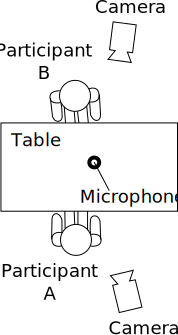
\includegraphics[width = 0.30 \columnwidth]{corpus/VideoCapturePlan.pdf}
\caption{Plan view of video capture equipment arrangement.}
\label{FigureVideoCaptureEquipment}
\end{figure}

Once both participants arrived in the laboratory, they were given only two instructions: to be seated and to communicate until told to stop. Having the participants seated reduces the amount of variation in body and head pose. Without this constraint, participants tend to turn away from the camera which makes facial tracking difficult. The experimenters were not visible to the participants during the recording. The participants were then allowed to talk without further experimenter interaction for 12 minutes. The conversations were of limited duration because the participants may begin to tire and change their behaviour. The instruction to communicate was considered necessary because the laboratory is not a normal place for socialising. The participants seemed to ignore their artificial surroundings and interacted in a natural fashion. The demographics of the participants in the four dyadic conversations are shown in Table \ref{ParticipantDemographics}. The number of conversations and duration was based the need to capture a range of \ac{NVC} behaviours without tiring the participants. The use of eight subjects is suitable for person independent cross validation testing with the majority of the data being available for training (87.5\% in training, 12.5\% in test). Using the person specific \ac{LP} tracker, more individuals and conversations also requires more person specific training to achieve acceptable tracking accuracy and additional resources required to organise and record the corpus. However, more participants results in an increased number of cross validation folds, which allows the standard deviation of the performance to be estimated more accurately. Less individuals in the corpus requires less training data for \ac{LP} tracking (see Appendix \ref{BackgroundLpTracking}), but results in a smaller proportion of data available for training in cross validation. Different cultural pairings were used in each conversation, which rules out the possibility of a study of cultural differences in expression within the TwoTalk corpus. Later chapters consider cultural perception differences, rather than expression differences caused by cultural background. Example frames from the corpus are shown in Figure \ref{FigureExampleCorpusFrames}.

%Samples in the recorded video corpus are informal, unfocused, without pragmatic purpose and topics changes occur in an unstructured way. This fits the description of causal conversation as previous discussed in Section \ref{BackgroundSocialContextUsedInTwoTalk}. 
%Many existing studies use specialised social situations, it is unclear to what extent these findings apply to applications outside the laboratory. Ideally, naturalistic recording of social interactions should take place in their normal location and context. However, it is hoped the near universality and flexibility of informal conversations that they can be recorded in the lab while still having a resemblance to social situations outside the lab.

\diffblock{
\begin{table}
\centering
\caption{Demographics for Conversation Participants in the LILiR TwoTalk Corpus. Abbreviations: UG is an undergraduate degree. M is a master's degree. Certain entries are omitted in cases where the participant was no longer contactable.}
\small
\begin{tabular}{ | c || c | c | c | c | c | c | c |}
\hline
Participant & Country   &  & Age   & Years UK &Education & Languages &  \\
            & of Origin &        & Years & Resident &          & Spoken & Natively \\
\hline
\hline
1008 & Nigeria & \male & 25 & 16 & M  & English & Yes\\
1011 & British & \male & 29 & 25 & UG & English & Yes\\
2008 & Spain   & \male &    &    &                &         & \\
2011 & British & \female  & 27 & 27 & UG & English & Yes\\
     &         &         &    &   &               & French & No \\
     &         &         &    &   &               & British Sign & No \\
3008 & Mexico & \male     & 29 & 5.5 & PhD & Spanish & Yes \\
     &        &           &    &     &     & English & No \\
3011 & Sri Lankan & \male & 25 & 6 & M & Bengali & Yes \\
     &        &          &    &   &             & English   & No \\
     &        &          &    &   &             & Hindi   & No \\
6008 & Indian & \male     & 27 & 1 & M & English & Yes \\
     &        &          &    &   &             & Hindi   & Yes \\
6011 & Ukranian & \female & 27 & 2 & M & Ukrainian & Yes \\
     &          &        &    &   &             & Russian & Yes \\
     &          &        &    &   &             & English & No \\
     &          &        &    &   &             & French & No \\
     &          &        &    &   &             & German & No \normalsize\\
\hline
\end{tabular}
\label{ParticipantDemographics}
\end{table}
}

Four conversations of 12 minutes length provide 48 minutes of conversation. The conversation was recorded by two cameras, resulting in 96 minutes of video. 
%As discussed in Section \ref{BackgroundWhyNvcAnnotationIsBoring}, annotation of \ac{NVC} and emotion is a time consuming and tedious process. 
%Individual \ac{NVC} signals vary from under a second to several seconds or more. 
For multiple annotators, the inter-annotator agreement for corpuses of emotion \cite{Reidsma2008} and \ac{NVC} is low. For this reason, each \ac{NVC} signal clip was rated by multiple annotators to reduce the effect of person specific factors. Much of the recorded conversations contain only passive listening, with no apparent \ac{NVC} displays, which is only marginally interesting. As Cowie \etal \cite{Cowie2009} observed, the distribution of signs is not uniform in human communication. 
%Given these considerations and limitation of resources that could be committed to annotation, the entire video could not be annotated. 
\thesiscomment{QUESTION: To what extent to others manually select a subset of their data? Examples?}
Sections of recordings that contained little or now activity were manually identified and excluded. The remaining sections of video contained potentially interesting behaviours. The annotators were not informed of the particular \ac{NVC} that was potentially present in clips of interest, so the \ac{NVC} content of the corpus was rated entirely by the annotators.
407 clips were selected as potentially of interest. The proportions of \ac{NVC}s that were thought to be present in the initial clip selection process is shown in Figure \ref{FigureManuallySelectedClips}. The different \ac{NVC} frequencies are due to the natural frequencies of occurrence of the various \ac{NVC} signals. An additional 120 randomly selected clips were also included to increase the variety of samples in the corpus. This may include common \ac{NVC} signals that were not considered in the questionnaire and also samples of null \ac{NVC} expression. This increases the richness of the videos shown to the annotators and prevents them reducing the problem to a hard assignment, 4 class problem which may influence the resulting annotation data. Both the manual and random sets of clips are combined, to form a final set of $\numClips=527$ clips with an overall duration of 38 minutes. The clip lengths used ($\lengthofclip=0.6$ to $10$ seconds, average $\overline{\lengthofclip}=4.2s$, standard deviation $\sigma(\lengthofclip)=2.5s$) are similar in duration to Lee and Beattie's work in discourse analysis \cite{Lee1998} (sample lengths of $\overline{\lengthofclip}=4.8s$, standard deviation $\sigma(\lengthofclip)=2.5s$). 
%The clips were presented to the annotators, but without informing them as to what the clip was thought to contain. 
If only total duration is considered, this data set is somewhat smaller than other data corpuses. For example, the emotionally labelled subset of the Belfast Naturalistic Emotional Database has a duration of 86 minutes \cite{DouglasCowie2003}, AMI Meeting corpus has 100 hours \cite{Carletta2007} and Madan's speed dating corpus has 350 minutes \cite{Madan2003}. However, these corpuses have different annotation methodologies and goals, and in many respects are not comparable with the TwoTalk corpus. Canal 9 is a large corpus (42 hours) but only a 10 minute subset is annotated for agreement and disagreement \ac{NVC}.
%Given that there are around 100 positive samples for each category of \ac{NVC} and many more negative samples, we expect that this will be sufficient for training and testing an automatic system.

\thesiscomment{DISCUSS duration of NVC in \cite{Verduyn2009}}

\begin{figure}
\centering
\includegraphics[width = 0.60 \columnwidth]{corpus/FigureManuallySelectedClips.pdf}
\caption[Number of manually selected and randomised clips in each of the NVC categories of interest.]{Number of manually selected and randomised clips in each of the NVC categories of interest. For \textit{agree}, \textit{understand}, \textit{thinking}, \textit{question} and \textit{random}, the number of clips are 109, 140, 93, 65 and 120 respectively.}
\label{FigureManuallySelectedClips}
\end{figure}

\thesiscomment{QUESTION: Several areas for improvement. Location, instructions, social context, selection of participants?}

\thesiscomment{QUESTION: Does changing the balance of clips presented to the user change their perception?}

\section{Design and Description of the Annotation Questionnaire}
\label{SectionSelectionOfNvcCategories}
\label{SectionDescribeQuestions}

%There are many approaches to coding inter-personal corpora.  This section describes the questionnaire used in this study along with a rationale for its design choices.

In attempting to encode \ac{NVC} signals, a system was selected that encompasses as many \ac{NVC} signals as possible, while making the annotation system easy for the annotators to use. In a similar manner to emotion, \ac{NVC} signals change over time and, due to the flexibility of human expression and human interpretation, a vast range of communication signals are possible. 
%An overview of related work is provided in Section \ref{BackgroundQuestionaireDesign}. 
%We use the common assumption that a complex system, \ac{NVC} expression in this case, can be expressed by a combination of more basic components, or in other words, that human communication is a superposition of one or more \ac{NVC} signals. 
However, the specific labels used for \ac{NVC} encoding need to be selected as the basis for annotation. 

%A corpus can be manually encoded based on a description of shape and appearance or in an interpretative sense, which considers the meaning or function of human actions \cite{Kipp2009}. For example, a particular set of muscle contractions (such as \ac{FACS} \cite{Ekman1978} or gaze and Duchenne smiles \cite{Lee1998}) is a descriptive model which can be objectively assessed, in contrast to estimating the intended meaning of a person's gesture which is interpretative. Because many practical applications of \ac{NVC} recognition require an interpretive encoding scheme, this approach is used in this thesis. Of course, it is possible to use descriptive encoding as an intermediate representation, before attempting to recognise interpretative labels and is a complimentary area of study.

An interpretative label is used to encode meaning in \ac{NVC}. An encoding scheme can have a ``categorical'' or ``dimensional'' encoding basis \cite{Cowie2005}. 
%Emotions may also be encoded using appraisal based methods (an observer evaluation determines the true label) \cite{Scherer1999}, but it is unclear if this can be applied to \ac{NVC}. 
Categorical systems rate events based on its similarity to a set of exemplars. Usually these exemplars are based on language that is easy to interpret (e.g. Ekman 6 basic emotions \cite{Ekman1972}). Abstract dimensional systems, which are not based on a simple similarity between an observed to an exemplar expression, attempt to represent a much broader range of events using abstract rating scales. Abstract dimensional encoding includes the commonly used scales activation and valence \cite{Devillers2005}.
%The range of possible meanings conveyed by \ac{NVC} signals is unknown and may be effectively unlimited. This implies that both the categorical and dimensional approach cannot comprehensively encode \ac{NVC}. 
Given the ease of use of exemplar NVC concept labels and the lack of any low dimensional, abstract encoding system for \ac{NVC} encoding, an prototypical (exemplar) \ac{NVC} basis was selected.

%As far as practically possible, categorical encoding of \ac{NVC} should to accurately encode natural conversation. 
Multiple \ac{NVC} signals may occur simultaneously and with a range of intensities. \ac{NVC} encoding needs to address these possibilities. 
%For example, nodding and winking can occur together but can be considered a superposition of nodding and winking. 
For this reason, the popular approach of using multi-class, hard assignment (mutually exclusive) labels is not suitable for capturing the nuances of \ac{NVC} signals. A high dimensional prototypical approach was adopted, which considers \ac{NVC} on multi-dimensional scales \cite{Kruskal1978} which can independently vary. This method is relatively easy to use while accurately encoding a subset of co-occurring \ac{NVC} signals.

%Because the physical actions of \ac{NVC} signals vary in time, the conveyed meaning varies in a similar fashion. 
For temporal annotation of video there are a few approaches that may be used:
\begin{itemize}
 \item One annotation strategy is to evaluate the video using a continuous input device in real time to form a temporally continuous annotation. This thesis considers the issue of temporally continuous to be distinct from being \continuous labels in an \ac{NVC} or emotion dimensional space, however a corpus may possess both properties as in the case of the FeelTrace system \cite{Cowie2000}. Dimensional encoding is typically used for encoding \continuous labels \cite{Nicolaou2011}, although it would be possible in principle to use temporally continuous categorical encoding. Temporally continuous encoding requires  specialised equipment and additional effort by the annotators.
 \item The alternative is to use individual clips rather than long uninterrupted videos. However, this raises the issue of how the start and end frame of clips are selected.
%As discussed in Section \ref{FigureVideoCaptureEquipment}, resource constraints dictated that annotation was performed on a subset of clips. 
\end{itemize}
To control the resources expended in annotation, short clips were manually extracted from the original video recordings and used as the basis for \continuous annotation in this study. This study is therefore not temporally continuous.

%The Ekman basic emotions were not used because this study is concerned with \ac{NVC}, not emotion. 
There is no standardised, comprehensive set of \ac{NVC} signals and little existing research in this area. In one of the few direct studies of \ac{NVC}, Lee and Beattie \cite{Lee1998} examined the use of gaze and Duchenne smiles in an \ac{NVC} context. However these \ac{NVC} signals do not have any obvious practical application. Another study, based on recognizing mental states, was conducted by el Kaliouby and Robinson \cite{ElKaliouby2004}. The mental states they studied were \textit{agreeing}, \textit{concentrating}, \textit{disagreeing}, \textit{interested}, \textit{thinking} and \textit{unsure}. Mental states are not necessarily expressed outwardly and can be expressed with or without communicative intent; this is in contrast to \ac{NVC} which is always communicative, outwardly expressed and intentional. The criteria used in this study for selection of \ac{NVC} signals to study were:

\begin{itemize}
 \item the signal should be an intentional \ac{NVC} action,
 \item they commonly occur in the social context used (i.e. casual chat/informal conversation),
 \item they may be potentially useful in one or more application and
 \item they may modify the meaning of the literal words used.
\end{itemize}

\begin{table}
\centering
\caption{Questions used in web based annotation of the LILiR TwoTalk corpus.}
\begin{tabular}{ | c | c | c | }
\hline
Question for Category & Minimum Rating & Maximum Rating \\
\hline
\hline
Does this person disagree or & Strong  & Strong  \\
agree with what is being said? & disagreement & agreement\\
(A score of 5 is neutral or not applicable.) & & \\
\hline
Is this person thinking hard? & No indication & In deep thought \\
\hline
Is this person asking & No & Definitely \\
a question? & indication & asking question\\
\hline
Is this person indicating they & No indication & Strongly  \\
understand what is being & or N/A & indicating\\
said to them? & & understanding\\
\hline
\end{tabular}
\label{CategoryLabels}
\end{table}

Based on the previous design decisions, the questionnaire is a quantised, multi-dimensional\footnote{Questionnaires can be used to collect multi-dimensional responses e.g. \cite{Tellegen2008}.} encoding using Likert scales of short video clips. The questionnaire presented to the annotators is summarised in Table \ref{CategoryLabels} and reproduced in Appendix \ref{ChapterQuestionnaire}. In this thesis, the 4 categories are abbreviated to \textit{agree}, \textit{thinking}, \textit{question} and \textit{understand}, and refer to the content of this questionnaire. The labels are exemplar based (in a similar fashion to the Ekman basic emotions), unlike activation and valence which are not exemplar based. This thesis uses dimensional labels that are tailored for the needs of \ac{NVC} encoding. As previously discussed in Section \ref{BackgroundQuestionaireDesign}, dimensional encoding is used in a wide variety of human behaviour annotation and is not limited to activation and valence.

As with el Kaliouby and Robinson, the \ac{NVC} labels of \textit{agree} and \textit{disagree} were used because these met the above criteria. Agreement signals are among the most prevalent of \ac{NVC} signals \cite{Bousmalis2009}. Agreement and disagreement are mutually exclusive messages, therefore these labels are expressed on a single dimensional scale. 
%This was later realised to be unnecessary because disagreement was rarely seen in the corpus and are discarded for the purposes of classification. However, other social situations may have frequent expressions of disagreement. 
The \ac{NVC} signal \textit{thinking} was used because it is a common and distinct behaviour in the corpus, based on an informal viewing of the corpus videos. Also, the tracking method used is very effective for eye movements and gaze is known to play a role in conversation turn taking \cite{Argyle1976}. The way gaze varies during thinking is culturally dependent \cite{McCarthy2006}, making it a potentially interesting \ac{NVC} signal when comparing different cultural perceptions of \ac{NVC} (see Chapter \ref{ChapterNvcRegression}). However, \textit{thinking} is arguably a mental state, as much as a true communication signal. 
%However, it is associated with a facial gesture which may be an intentional action to regulate the conversation.
 \textit{Question} is included because it drastically changes the meaning of an utterance, which may have applications in multi-modal speech recognition. The inclusion of \textit{question} was debatable, because while questions can be recognised by changes in voice intonation, it was unknown if visual recognition of a question was even possible. \textit{Understand} is another common signal which regulates conversation and has both verbal and non-verbal components. 
%The number of \ac{NVC} signals studied was limited because of the limited resources available for annotation of the data. 
The \ac{NVC} signals of \textit{agree} and \textit{understand} express attitudes and are therefore social signals. While \textit{thinking} and \textit{question} are likely to have a role in regulating conversation flow, their exact role and significance is uncertain and their status as social signals is current uncertain.

A questionnaire can collect dimensional responses may have labels values that are either discrete (quantised) or continuous. Continuous value data may be collected by marking a point on a continuous line using either a written mark or computer input \cite{Treiblmaier2011}. The term ``continuous value'' does not exclusively apply to annotations with continuous temporal traces, such as FeelTrace\footnote{Human behaviour may either be encoded as either discretised or continuous in terms of annotation labels: ``When discretised dimensional annotation is adopted (as opposed to continuous one), researchers seem to use different intensity levels'' \cite{Gunes2011}}. The concept of ``continuous emotional space'' is expanding beyond activation and valence, with Hupont \etal \cite{Hupont2013} using a 2{D} continuous value space (\textit{evaluation} and \textit{activation}) without considering the temporal dimension. Liscombe \etal \cite{Liscombe2003} used a web-based survey to gather \continuous emotion annotation data for each utterance in an audio corpus. Discrete binary labels might simply be ``\ac{NVC} is expressed'' and ``\ac{NVC} is not expressed''. Binary discrete labels were used by Lee and Beattie \cite{Lee1998} in their discourse analysis of \ac{NVC}. Discrete labels can also be used in dimensional annotation and may be encoded using integer values. Continuous valued labels are dimensional ratings that have non-integer values and are commonly used in psychological research \cite{Nicolaou2011, Wollmer2009, Cowie2000}. A Likert scale \cite{Likert1932} is a common psychometric questionnaire in which a ordinal rating can be provided between two extreme choices. Taking the mean of multiple annotators results in a value that can take non-integer values and is therefore a \continuous variable. While some concerns have been raise as to the validity of using a Likert scale as an interval-level measure with parametric statistics \cite{Jamieson2004}, a number of studies have examined the use of Likert scales as an interval-level measure and found it to be a reliable research tool \cite{Rasmussen1989} \cite{Owuor2001}. Both Carifio and Perla \cite{Carifio2007} and Norman \cite{Norman2010} argue that it is time to put the controversy of the use of the Likert scale as a interval-level measure in the past because of the repeated demonstration of the worth of using Likert scales with parametric statistics, such as mean and variance.
%A binary label is less expressive than a continuous scale. 
%A continuous scale was used to avoid losing information that may be relevant to a practical application. However, 
A Likert scale was used in this study as this retains intermediate intensity expressions while being applicable to an Internet based survey.

%This section has described the TwoTalk corpus and questionnaire. The following section describes how the annotation data was collected.

\section{Multi-observer Annotation of NVC}
\label{SectionMultiCultitureAnnotation}

%The previous sections have described how the questionnaire was designed and how the data corpus was recorded. 
%To use supervised learning on this corpus, the sample labels need to be determined.
Inter-annotator agreement for inter-personal events is typically low. (``These annotations [of subjective corpura] often have a quite low overall level of inter-annotator agreement'' \cite{Reidsma2008}) This is also likely to be true for \ac{NVC} perception. \ac{NVC} perception is highly subjective and partly dependent on person specific, social and cultural factors (see Section \ref{BackgroundWhatFactorsInfluenceNvc}). Multiple annotators are used in an attempt to reduce the effect of interpersonal variations. Other techniques to improve inter-annotator agreement were not employed (e.g training the annotators, having the annotator previewing the corpus, multiple ratings on individual clips by individual annotators, subject normalisation). This was due to the limitations in resources needed to conduct such a study and the technical limitations of crowd sourced annotation.
The differences in perception between cultures are not considered in this chapter, but this issue is revisited in Chapter \ref{ChapterAnnotation}.

\begin{figure}[tb]
\centering
\includegraphics[width = 0.5 \columnwidth]{corpus/crowdflower-survey.png}
\caption[A typical page of the annotation questionnaire, which is accessed using a web browser.]{A typical page of the annotation questionnaire, which is accessed using a web browser. Each clip is annotated individually. The user has the ability to replay the video and is required to respond to the four \ac{NVC} questions.}
\label{FigureAnnotationSurveyScreenshot}
\end{figure}

The questionnaire was presented to annotators using a computer based system. These are commonly used for annotation of video \cite{Eckhardt2009, Cowie2000, Tarasov2010} and allow participants to complete the survey at their own convenience, rather than having to attend an organised session. A web based system was used, because the system could be remotely accessed using a web browser. A web page displayed one or more videos and each could be viewed one or more times. Under each video were the four annotation \ac{NVC} categories selected in Section \ref{SectionDescribeQuestions}. The user viewed the video clip and marked their answer using the mouse or keyboard. The order of the videos was randomised to reduce the possible effect of the video display order on the annotation data. A typical view of the annotation web site is shown in Figure \ref{FigureAnnotationSurveyScreenshot}. The videos were presented to the annotators with both visual and audio information. By presenting both, it was hoped that the most natural and realistic rating would be achieved. 
%Most, but not all \ac{NVC} information expressed in the visual domain (see Section \ref{BackgroundHowIsNvcExpressed}). 
%For this reason the automatic systems discussed in this thesis use visual information only. 
%Since not all the information that might be relevant to determining what \ac{NVC} is present, it might be expected that the automatic system will have some difficulty in correctly identifying types of \ac{NVC} that rely on an audio component (e.g. \textit{question}).

Allowing users to perform the annotation task with no supervision risks the participants not completing the annotation task as instructed.
%, for example having the audio disabled when rating the videos. 
The annotators were unpaid volunteers and were motivated by interest, loyalty or duty and were expected to generate relatively good quality data. Another approach used is to pay people to perform the annotation but this can lead to quality issues, which are addressed in Section \ref{SectionNeedToFilter}. Chapter \ref{ChapterAnnotation} addresses collecting annotation data from observes based in different cultures.

%Once the annotation system was designed and implemented, annotators began to view and rate examples of \ac{NVC} signals. The next section provides an analysis of their responses.

\section{Analysis of Human Annotators}
\label{SectionAnalysisOfHumanAnnotation}

\begin{figure}[tb]
\centering
\includegraphics[width = 0.5 \columnwidth]{corpus/demographicLocation.pdf}
\caption{Self-reported primary culture for annotators.}
\label{FigureDemographicLocation}
\end{figure}

Thirty one annotators participated in rating samples of \ac{NVC} ($\numAnnotators = 31$). Because expression and perception is dependent on cultural context, gender and personality differences (see Section \ref{BackgroundWhatFactorsInfluenceNvc}), it is relevant to consider the demographics of the annotators. Although all annotators were UK residents, some annotators had a separate primary cultural background. Annotators were mostly 21-30 years of age, with a science or engineering background (see Figure \ref{FigureDemographicAge} and \ref{FigureDemographicWork}). As can be seen in Figure \ref{FigureDemographicLocation}, the vast majority of annotators had a UK based cultural background. 
%Considering this, and the other annotators exposure to UK culture, it is likely that the cultural background of the annotators will only be a minor factor in any differences between annotators. However, the annotation data collected is from a single cultural perspective.
Annotation by distinct cultural groups is discussed in Chapter \ref{ChapterAnnotation}. The majority of respondents were male (see Figure \ref{FigureDemographicGender}). 
%The existence of two distinct groups among the annotators, each having a different perception of \ac{NVC} signals, might lead to two distinct clusters of annotation results. 
%The next section discusses how this may be reduced to a simple label. 
%The demographic questionnaire also asked about the annotators field of work. 
%Terracciano \etal \cite{Terracciano2003} found there is a relationship between personality and emotion perception. The role of personality is thought to influence the choice of career, although that role not well understood \cite{Vuust2010}. 
%It would be interesting to discover if there is a connection between \ac{NVC} perception based on career. 
It might be beneficial to include a personality questionnaire in future annotation projects to enable investigation of personality in a more explicit way. %The \ac{NVC} ratings provided by the annotators will now be considered.

\begin{figure}[tb]
\centering
\includegraphics[width = 0.60 \columnwidth]{corpus/demographicAge.pdf}
\caption{Self-reported age for annotators.}
\label{FigureDemographicAge}
\end{figure}

\begin{figure}[tb]
\centering
\includegraphics[width = 0.60 \columnwidth]{corpus/demographicWork.pdf}
\caption{Self-reported sector of employment for annotators.}
\label{FigureDemographicWork}
\end{figure}

\begin{figure}[tb]
\centering
\includegraphics[width = 0.5 \columnwidth]{corpus/demographicGender.pdf}
\caption{Self-reported gender for annotators.}
\label{FigureDemographicGender}
\end{figure}

The vast majority of annotators did not rate every video clip because \ac{NVC} annotation is time consuming and tedious. On average, each annotator rated 70 video clips, from a possible maximum of 527 clips. Each clip required all four \ac{NVC} signals to be rated. For the \ac{NVC} category \textit{thinking}, 2182 individual ratings were provided by the annotators, distributed across the corpus's 527 video clips. This corresponds to 4.1 ratings per video clip. 
%Having multiple ratings on a single question on a single \ac{NVC} video clip should reduce the effect of person specific \ac{NVC} perception. The other \ac{NVC} signals had a similar level of response. 

\begin{figure}[tb]
\centering
\includegraphics[width = 0.5 \columnwidth]{corpus/ratingof4.pdf}
\caption[Histogram of Average Rating based on multi-annotators.]{Histogram of Average Rating based on multi-annotators. Blue thin line is agreeing, magenta thick line is thinking, black dot-dashed line is understanding and red dashed line is questioning. Zero is a neutral score and 10 is strongly showing the communication signal. Disagreement ratings have been omitted.}
\label{RatingScoresFigure}
\end{figure}

%The questionnaire considers \ac{NVC} signals as varying in intensity from strongly showing a signal to no indication of an \ac{NVC} signal. The ratings were provided on a pseudo-continuous scale with intermediate intensity emotions receiving a score between extremes. 
Not all \ac{NVC} signs occur with the same frequency or intensity. Figure \ref{RatingScoresFigure} shows the distribution of \ac{NVC} intensity for the annotated videos. The frequency of \ac{NVC} occurrence in these videos almost certainly differs from unedited video, because the video clips in the corpus were specifically selected to include interesting \ac{NVC} examples and to avoid inactive sections. \textit{Question} \ac{NVC} has a strong peak at zero, indicating the majority of video clips do not contain this signal. 
%This is unsurprising, because the manually selected clips had relatively few examples of \textit{question} \ac{NVC} (see Figure \ref{FigureManuallySelectedClips}). 
\textit{Agree} and \textit{thinking} \ac{NVC} have a similar peak near ``no \ac{NVC} signal'', but differ from \textit{question} by having a minority of clips of intermediate intensity. \textit{Understand} \ac{NVC} has a relatively uniform frequency distribution, with some weak, intermediate and strong examples. Intense expression is rare for the \ac{NVC} signals considered in this work. Combining multiple individual annotator ratings to a single vector label will now be considered.

\section{Analysis of Mean Ratings}
\label{SectionAnalysisOfMeanRatings}

Annotator ratings are provided for each of the \ac{NVC} categories:

\begin{align}
\nvcCategory \in \setCategories = \{agree, understand, think, question\}
\end{align}

%For each video clip, the annotation produces a set of ratings for each \ac{NVC} category. 
%The number of annotator ratings is variable, however the supervised learning paradigm assumes each sample has a single label. 
For supervised learning, the individual ratings need to be reduced to a single consensus 4{D} label for each clip. This is performed by taking each \ac{NVC} quantised, dimensional rating and calculating the mean (similar to \cite{Tarasov2010, Wollmer2009}), which results in a \continuous label. The vector containing the number of annotation ratings for $\numClips$ clips is defined as $\numAnnotatorsOnClip \in \mathbb{N}^{\numClips}$. The ratings for clip $\clipId \in \{1...\numClips\}$, annotated for \ac{NVC} signal category $\nvcCategory$, is designated as matrix $\rawAnnotation_{\nvcCategory,\clipId}$ of size ${4 \times \numClips}$. $\rawAnnotation_{\nvcCategory,\clipId}$ comprises of a set of tuples, containing ratings $\ratingOfClip_i \in \mathbb{R}$ and corresponding annotator indices $\annotatorOfRating_i \in \{1...\numAnnotators\}$:
%($i \in \numAnnotatorsOnClip_{\clipId}$)
%$\rawAnnotation^{\nvcCategory}_{\clipId} \in \mathbb{R}^{\numAnnotatorsOnClip_{\clipId}}$
\begin{align}
\rawAnnotation_{\nvcCategory,\clipId} = \{(\ratingOfClip_i, \annotatorOfRating_i)\}_{i=1}^{\numAnnotatorsOnClip_{\clipId}}
\end{align}

The 4 \ac{NVC} categories and can be summarised into a consensus vector $\clipConcensus \in \mathbb{R}^{4 \times \numClips}$, $\nvcCategory \in \setCategories$:

\begin{align}
\clipConcensus_{\nvcCategory, \clipId} = \frac{\displaystyle\sum\limits_{i=1}^{\numAnnotatorsOnClip_{\clipId}} \{\ratingOfClip_i: (\ratingOfClip_i, \annotatorOfRating_i) \in \rawAnnotation_{\nvcCategory,\clipId}\}}{\numAnnotatorsOnClip_{\clipId}}
\end{align}

%For a specific clip, a four \ac{NVC} category consensus rating is found:

%\begin{align}
%\clipConcensus(\rawAnnotation)_{\clipId} = [\clipConcensus(\rawAnnotation)^{agree}_{\clipId}, \clipConcensus(\rawAnnotation)^{understand}_{\clipId}, \clipConcensus(\rawAnnotation)^{thinking}_{\clipId}, \clipConcensus(\rawAnnotation)^{question}_{\clipId}]
%\end{align}

This simplification assumes that inter-annotator differences are not significant for the intended application and that the annotator ratings are symmetrically distributed. However, human perception of \ac{NVC} depends on many factors (see Section \ref{BackgroundWhatFactorsInfluenceNvc}). The bulk of this thesis attempts to create and evaluate an automatic system that produces a prediction in a similar fashion to a human annotator. This chapter assumes the annotators form an approximately self-consistent group because of the demographic similarity of the annotators (see Section \ref{SectionAnalysisOfHumanAnnotation}).
% and any deviations in annotation are approximately symmetrically distributed. 
Therefore, using the rating mean to determine a consensus is valid in this case. However, it is important to remember the limitations of using the mean consensus, and specifically that taking the mean of non-homogeneous groups risks over-simplification of the problem. Chapter \ref{ChapterNvcRegression} considers the case of training an automatic system when multiple distinct groups of annotators exist.

An alternative to using the mean rating is to take a set of multiple annotator rating data and use a subset of clips in which there is agreement, as done by el Kaliouby and Robinson \cite{ElKaliouby2004}. This approach was not used, because it ignores clips in which there is low inter-annotator agreement.
%, but a broad coverage - including hard to rate clips - may be important for any practical application. The issue of dealing with separate annotator groups is raised in Chapter \ref{ChapterAnnotation}, as well as examine the case for treating cultures as separate label sets.

\begin{table}[tb]
\centering
\begin{tabular}{ | c || c | c | c | c | }
\hline
& Agreeing & Understanding & Thinking & Questioning \\
\hline
\hline
Agree & 1 & & &\\
Understand & 0.46 & 1 & &\\
Thinking & -0.21 & -0.23 & 1 &\\
Question & -0.18 & -0.40 & 0.06 & 1 \\
\hline  
\end{tabular}
\caption{Correlation coefficients of the mean ratings $\clipConcensus$ for each category.}
\label{CorrelationOfCategoriesTable}
\end{table}

%As discussed in Section \ref{SectionSelectionOfNvcCategories}, we treat the expression of complex \ac{NVC} as a superposition of more basic \ac{NVC} signals. However, 
The selected \ac{NVC} categories do not necessarily vary independently of each other. A linear dependence of two continuously varying signals can be found by calculating the Pearson correlation coefficient $\correlFunc$. The Pearson correlation coefficient $\rho$ for vectors $\textbf{x} \in \mathbb{R}^{n}$ and $\textbf{y} \in \mathbb{R}^{n}$, is defined as (adapted from \cite{Weisstein2008}, for a population, $i=\{1..n\}$):

\begin{gather}
\correlTemp(\textbf{x},\textbf{x}) = \displaystyle\sum\limits_{i=0}^n {\textbf{x}_i}^2 - n\bar{\textbf{x}}^2\\
\correlTemp(\textbf{y},\textbf{y}) = \displaystyle\sum\limits_{i=0}^n {\textbf{y}_i}^2 - n\bar{\textbf{y}}^2\\
\correlTemp(\textbf{x},\textbf{y}) = \displaystyle\sum\limits_{i=0}^n {\textbf{x}_i \textbf{y}_i} - n\bar{\textbf{x}}\bar{\textbf{y}}\\
\correlFunc (\textbf{x},\textbf{y})^2 = \frac{{\correlTemp(\textbf{x},\textbf{y})}^2}{\correlTemp(\textbf{x},\textbf{x}) \correlTemp(\textbf{y},\textbf{y})}
\label{EqnPearsonsCorrelation}
\end{gather}

\thesisstatement{Some pairs NVC category annotator responses are correlated}

where $\bar{\textbf{x}}$ and $\bar{\textbf{y}}$ are the mean values of $\textbf{x}$ and $\textbf{y}$ respectively. The value of $\rho$ gives an indication of the correlation between two signals. $\rho=1$ is perfect positive correlation, $\rho=0$ indicates no correlation and $\rho=-1$ indicates perfect negative correlation. The correlation between different \ac{NVC} signals is shown in Table \ref{CorrelationOfCategoriesTable}. The highest magnitude correlation score is between \textit{agree} and \textit{understand}, with a score of $\rho=0.46$. This is a relatively weak correlation but significant enough to say there is a relationship between these signs. This also confirms our intuitive expectation, because if a person wishes to indicate agreement, this necessarily implies they also want to convey that they understand. The next highest magnitude score is for \textit{understand} and \textit{question} at $\rho=-.40$. Being a negative correlation, this reflects that these signals are partially mutually exclusive; when a person is asking a question, they are unlikely to be conveying that they understand (and visa versa). Finally, the lowest magnitude score is for \textit{thinking} and \textit{question}, having a correlation of $\rho=0.06$. This implies these \ac{NVC} signals occur relatively independently of each other.

This analysis is interesting, because if there are many \ac{NVC} signals that are interrelated, it can imply that dimensionality reducing techniques can be applied without loss of information. 
%However, only a limited subset of \ac{NVC} signals is considered, so dimensional reduction of labels is not attempted in this work. Also, knowing which \ac{NVC} signals are independent and which are mutually exclusive is different from a multiclass approach, which assumes every class is mutually exclusive. 
The \ac{NVC} signals \textit{agree} and \textit{understand} often co-occur, therefore an approach using a single discrete class label would be problematic for \ac{NVC} recognition.

\thesiscomment{DISCUSS Equate neutral expression with no NVC being sent? Show examples? What about the possibility of sending NVCs not included in this study during inactivity?}

%This section has discussed the annotations and demographics provided by the volunteers. The next section concludes this chapter and outlines how it will be used for supervised learning.

\thesiscomment{QUESTION: Run our online tracker on these sequences? It should fail?}

\begin{figure}[tb]
\centering
\includegraphics[width = 0.80 \columnwidth]{corpus/AnnotatorCorrelHist.pdf}
\caption{A histogram of Pearson's correlation between an annotator's ratings and the mean of all other annotators' ratings. Some annotators did not rate enough data to compute a valid correlation and were excluded from this figure.}
\label{FigureAnnotatorCorrelationWithConc}
\end{figure}

The ratings for each annotator are compared to the mean of the other annotators. This provides a measurement of inter-annotator agreement. Figure \ref{FigureAnnotatorCorrelationWithConc} shows a histogram of the number of annotators at different levels of agreement with the cultural consensus. This shows that some annotators are in close agreement with the cultural consensus, while others are less so. For all 31 annotators, the average correlation with consensus is $0.47$. Inter-annotator agreement is discussed again in Section \ref{SectionAnnotationFilterMethod} in context of removing outlier annotators.

Correlation is used as the primary measurement of agreement of survey data in this study. The use of the popular Cronbach's Alpha is not a suitable measure of agreement or internal consistency \cite{Sijtsma2009, Revelle2009, Sijtsma2009b}, with Green and Yang calling for it's general use should be discouraged \cite{Green2009}. This metric is therefore not used in this thesis. Also, the habitual use of a particular threshold (such as the commonly used value of 0.7 or 0.8) to determine if a questionnaire validity risks over-emphasising the problem of random noise, to which machine learning techniques are somewhat robust, and ignoring the problem of systematic errors by the annotators (See Chapter 3 of Reidsma \cite{Reidsma2008Thesis}). Reidsma argued that using corpus data with a higher inter-annotator agreement generally leads to better performance in automatic recognition.

\section{Conclusion}

This section has described a corpus that comprises of recordings of two person, informal conversations. Minimal experimental constraints were used to maximised the natural and spontaneous character of the social situation. Annotation was performed on video clips to encode the conversation meaning. The annotators were shown the video clips with audio. The data was collected based on quantised, dimensional Likert questions. Based on this, a consensus label based of the mean of multiple annotators was calculated for each question which resulted in \continuous labels. This consensus annotation data will be used in later chapters of this thesis as the basis for an automatic system.

Currently, the cultural background of the \ac{NVC} encoders and the annotators is not well controlled. To understand and distinguish between personal and cultural differences, it would be beneficial to have recordings from distinct cultures and have them annotated by multiple cultures. 
%The corpus can then be analysed to find the different usages and frequencies of \ac{NVC} gesture. Also, cultural differences in perception of \ac{NVC} signals can be examined. 
This use of culturally distinct annotators is discussed in Chapter \ref{ChapterAnnotation}.

The finding that \ac{NVC} labels often co-occur and do not vary independently raises the question as to redundant information in \ac{NVC} labels. If \ac{NVC} can be expressed in a lower dimensional space, the annotation task and automatic recognition problem are both simplified. However, the \ac{NVC} labels used are not comprehensive and further work is needed to find an \ac{NVC} annotation system with a broader coverage of meaning.

The corpus was recorded in a laboratory environment. It is likely that more naturalistic data would be obtained by recording data in an environment in which an automatic system is expected to be deployed. Some data sets that attempt this have recently become available, such as the D64 Multimodal Conversational Corpus being recorded in a domestic environment. %When an automatic system is trained on data that is representative of an application, it will have improved performance.
The next chapter describes an automatic \ac{NVC} classification system based on the data collected in this chapter.

\include{nvcclass/nvcclass}

\begin{savequote}
The meeting of two personalities is like the contact of two chemical substances: if there is any reaction, both are transformed.
\qauthor{Carl Jung}
\end{savequote}

\chapter[Interpersonal Coordination in NVC]{Interpersonal Coordination in NVC}
\label{ChapterBackchannel}
\label{SectionBackchannelIntro}

\thesiscomment{MAIN POINT OF CHAPTER: Facial behaviour mirroring is observed and quantitatively measured, which provides a basis for automatic \ac{NVC} recognition using backchannel signals.}

\thesiscomment{WHAT we do}

\thesiscomment{HOW we do it}

\thesiscomment{RESULTS, IMPACT and NOVELTY}

The previous chapter considered automatic \ac{NVC} recognition based on visual information of the sender or ``encoder'' of an \ac{NVC} signal (encoder in this case does not refer to the annotators or automatic encoding but rather to the observed subject exhibiting a behaviour \cite{Lanzetta1970}). This chapter considers the behavioural associations between an \ac{NVC} encoder and the \ac{NVC} perceiver, and describes a study of recognising \ac{NVC} signals based on the behaviour of the \ac{NVC} perceiver. In natural two person conversations, the behaviour of one participant influences the other participant. 
%This effect has been previously studied for both verbal and non-verbal communication. 
Usually, people take turns to speak in a conversation. In a dyadic (two person) conversation, the information flow is bi-directional. In a particular speech turn, the speaker's communication is referred to as the ``forward'' channel. The person listening to the speaker also responds to the speaker, primarily using non-verbal communication, and this communication is known as the ``backchannel''. Backchannel communication allows a listener to influence a conversation without verbally interrupting or taking a conversation turn. The forward and backchannel communications occur simultaneously and can vary in style across cultures. For this reason, both subjects in a dyadic conversation can be thought of as both an encoder and perceiver of \ac{NVC} simultaneously and this is bi-directional flow of information exploited in this chapter.

In natural conversations, participants often mimic or mirror behaviours being expressed by the other person. Mimicry or ``behaviour matching'' occurs when two or more people show similar body configurations \cite{Bernieri1991}. For example, if one person touches their face during a conversation, the other person is more likely to do so. 
%This coupling of behaviour is distinct from backchannel communication, because if often occurs without 
Another class of behaviours is performed in a common rhythm, with the starting and ending of movement being simultaneous. This is known as ``synchrony'', which comprises of corresponding rhythms, simultaneous movement and the smooth meshing of interaction \cite{Bernieri1991}. Together, synchrony and behaviour matching are considered as ``interpersonal coordination''. The phenomena of behaviour mirroring and synchrony are not disjunct and can occur at the same time \cite{Delaherche2012}. These effects raises the possibility that a perceiver's behaviour in response to an \ac{NVC} signal may be useful in \ac{NVC} recognition. Based on this idea, backchannel information for automatic \ac{NVC} recognition is studied and evaluated. 

The main contributions of this chapter are:

\begin{itemize}
 \item A method for automatic identification of certain types of interpersonal coordination in the deformation of the face during casual conversation. This method is applied to recorded videos and the results are analysed.
 \item A study of \featureGeneration methods for \ac{NVC} classification that identifies \ac{NVC} signals observed in the forward channel, based solely on backchannel feature data.
\end{itemize}

The next section outlines previous studies that are related to this work. Section \ref{SectionMirrorBehaviour} investigates the inter-person coupling of face deformations in conversation. A automatic system to classify \ac{NVC} based on backchannel cues is described in Section \ref{SectionClassificationBackchannel}.

\section{Related Research}
\label{BackgroundNvcIsCoupled}

Backchannel is a form of human communication which has been relatively little studied. The first mention of it is probably by Yngve \cite{Yngve1970} where he observed that the backchannel allows a listener to express non-verbal or brief verbal speech to influence a conversation, without taking a conversational turn. Even prior to this, gaze was thought to be used in conversation regulation by Kendon \cite{Kendon1967}. Backchannel signals provide a way for a listener to signal agreement or disagreement, as noted by Bousmalis \etal \cite{Bousmalis2009}. Backchannels differ across cultures, with some cultures having a higher frequency of backchannel signals \cite{White1989}.

Human behaviour may also be coupled during conversations, besides consciously performed communication acts. Various studies have tried to quantify this behaviour (see Reidsma \etal \cite{Reidsma2010} and Delaherche \cite{Delaherche2012} for a review). Chartrand and Bargh \cite{Chartrand1999} found that people in conversation tend to adopt the same posture, mannerisms and expression. Similar observations have been found for limb movement, and many aspects of speech, but these effects are dependent on social context \cite{Frith2009}. 
%Patterns in human communication have been studied using automatic means, although this work is at an early stage. 
Several studies have used automatic recognition of synchrony (see \cite{Delaherche2012, Sun2012} for reviews). There is a many different feature extraction techniques and measures of synchrony. Richardson \etal \cite{Richardson2007} studied gaze and noted that when two subjects are observing the same scene, their gaze motion is coupled. They found that behaviour was most strongly coupled between synchronised inter-person movements, but also found evidence of gaze coupling occurring after a delay of up to about 3 seconds. The social situation has an impact on the types of mimicry that occur \cite{Bourgeois2008}. Coupled human behaviour may be useful for automatic recognition. Until recently, there have been no approaches that use backchannel communication. Morency \cite{Morency2011} studied automatic recognition based on backchannel signals and attempted to predict listener responses to a speaker. Okwechime \etal \cite{Okwechime2011} used a-priori data mining to find behaviour patterns in conversation and considered both audio and visual modalities. This study was performed in controlled social situations to elicit interested or disinterested behaviours by the listeners and social context based behaviour differences were identified. %The following section uses geometric features introduced, in the previous chapter, for automatic analysis of coupling of human expression.
Ramseyer and Tschacher \cite{Ramseyer2008} used correlations in difference images to find cross-correlated patterns with a time offset of $\pm$5 sec. They used time shuffled windows to produce non-coordinated behaviour data to determine the extent of cross correlation cause by the null hypothesis. No existing studies consider automatic detection of interpersonal coordination in facial behaviour, although Sun \etal are working towards this goal \cite{Sun2012}.

The MAHNOB HMI iBUG Mimicry dataset (shortened to MHi-Mimicry-db) \cite{Sun2011} contains recordings of dyadic conversations in role play and discussion situations for the purposes of analysing mimicry behaviour. This dataset is significantly larger and more complex than the TwoTalk corpus, containing about 12 hours of records of 40 subjects using 15 video cameras and 3 audio channels. The corpus was manually annotated to produce labels to investigate how mimicry is expressed, if it is intentional or unintentional and the social signal being expressed. Intentional signals were also labelled in terms of the goal of the mimicry. The camera synchronised error was ``well below'' 20 $\mu$sec. The two social situations contained in the MHi-Mimicry-db were a political discussion with a confederate and a role play concerning renting a room to a potential lodger. These scenarios were selected to test specific existing hypothesises of human behaviour. Both were dyadic conversations were conducted in a laboratory. The MAHNOB Mimicry dataset was not available at the time this part of the study was conducted. The following section focuses on interpersonal coordination that may be automatically identified without the use of annotation.

\section{Coupling in Interpersonal Coordination during Informal Conversation}
\label{SectionMirrorBehaviour}

This section describes an automatic method to analyse coupling in facial behaviour. Because this correlation based method is sensitive to both rhythmic and non-rhythmic behaviours, certain types of both mimicry and synchrony behaviours will be detected. Correlation being used as a measure of mimicry can be understood in terms of it's mirroring property. Two people tend to reflect or mirror each others body positions and behaviours. By analogy, correlation is a way of measuring the  extent of ``mirroring'' between two variables. This makes the Peason's correlation suitable for finding some types of coupled behaviours. A more detailed justification of using Pearon's correlation is provided in Appendix \ref{ChapterMimicryColleration}.

Correlation of simultaneous frame features is not sensitive to types of mimicry in which the response behaviour is delayed for a longer time than the duration of the trigger behaviour. The class of behaviours that can be detected by the approach described here will be referred to as ``coupling''. Automatic methods can provide a more comprehensive analysis than can be achieved by manual methods because automatic approaches can scale to large quantities of video data.
% than can be collected by human based encoding (using gesture events, \ac{FACS} or similar). 
%This may be an important as a tool in further research to understand human behaviour. 
The next section describes the method, based on tracking, feature extraction and Pearson correlation. Section \ref{SectionCouplingResults} shows the results and discusses their significance.

\subsection{Methodology}

Using the four dyadic conversations recorded as part of the corpus (see Section \ref{SectionDescriptionOfTwoTalkCorpus}), behaviour patterns that are common to both participants can be identified. The cameras used to record the corpus are genlocked to ensure synchronisation of video frames. Genlock is a common technique to synchronise cameras using a generator signal. The genlock signal was provided by a Tektronix TG700 Multi-Format Video Generator. The cameras were all of the same type; this greatly simplifies achieving accurate synchronisation. Based on informal tests performed by the broadcast engineer responsible for maintaining the system, the camera jitter measured to be was less than one microsecond (the level of jitter in the camera synchronisation was smaller than measurable using the available equipment). The features introduced in the previous chapter are used, \textit{geometric-a}, which are based on distances of pairs of feature trackers (Section \ref{SectionGenerateAlgorithmic}). These features are applied to the face and non-facial behaviour is not considered. %Previous research has found that there are non-facial behaviours that are coupled but this thesis is limited to considering facial behaviour. 
Clearly, some areas of the face will not be coupled e.g. when one person speaks, it is usual for the other person to listen and not to move their mouth in the same way. To identify coupled behaviour, the variation of each feature for both speakers in a conversation are compared using Pearson's correlation $\correlFunc$ (see Equation \ref{EqnPearsonsCorrelation}). If features are highly correlated, this indicates that they are closely coupled. A low correlation indicates the features vary independently. As the correlation is performed on simultaneous frames, it will only capture mimicry between individuals if the offset between the occurrences is less than its duration. While this approach is insensitive to more delayed mimicry, it should identify shorter term mirroring of behaviour (see Appendix \ref{ChapterMimicryColleration}). The correlation score corresponds to the strength of coupling of the behaviour. The original video records are used because it increases the quantity of data available for analysis. The feature vectors $\frameFeatureMatrix$ of two participants $A$ and $B$ are compared $A, B \in \{1008, 1011, 2008, 2011, 3008, 3011, 6008, 6011\}$. For feature component $i \in \{0...\numFeatures\}$, the correlation $\dyadicCorrelation$ is ($\frameFeatureMatrix^A_i \in \mathbb{R}^{\numSeqFrames}$, $\numSeqFrames = 12 \times 60 \times 25 frames$, $\dyadicCorrelation^{A,B}_i \in \mathbb{R}$):

\begin{gather}
\dyadicCorrelation^{A,B}_i = \correlFunc(\frameFeatureMatrix^A_i, \frameFeatureMatrix^B_i)
\end{gather}

If a behaviour is performed as a reaction, there may be a time delay between the behaviours. Each frame of one participant is compared to a simultaneous frame of the other participant taken using a second camera. This makes this approach sensitive to synchronised behaviours but insensitive to mirroring behaviours that have a temporal offset and short duration. For example, if one person adopts an expression for several seconds and the second person quickly adopts the same expression, this will be found using the correlation of features. The correlation coefficient is limited to measuring linear relationships. It is quite possible that reliable, non-linear patterns of human behaviour may exist. Another limitation of this approach is that this considers only variations in shape but it is possible that patterns in human behaviour may be found if speed or acceleration of the face is also considered.

For this test, corresponding features are compared (e.g. position of left eye in both participants) rather than different areas on the face (e.g. left eye for one subject and mouth opening for the second subject). This constraint makes the system focus primarily on mirroring behaviour. Because the strongly coupled areas of the face are most interesting, the highest scoring feature $i^{A,B}_{max}$, with correlation $\dyadicCorrelation^{A,B}_{max}$, is found:

\begin{gather}
i^{A,B}_{max} = \argmax_{i}{\dyadicCorrelation^{A,B}_i}
\end{gather}

This feature corresponds to a specific area on the face in which the behaviour is coupled. However, there is a possibility that features vary and may coincidentally vary together. It can be difficult to distinguish weak causal relationships with coincidental inter-relationships. To examine this possibility, the correlations of features $\dyadicCorrelation_{max}$ for individuals that were not in the same conversation was also computed. Apparent correlations between unrelated conversations can be regarded as coincidental.
%, except if there is a inter-conversation pattern. An example of patterns that occur across conversation might be if head position varies in time due to tiredness. However, it is thought that this effects will not be significant compared to intentional gestures.

%The next section presents the results of this approach and discusses their significance.

This method is similar to Ramseyer and Tschacher \cite{Ramseyer2008} but contains some important differences:
\begin{itemize}
 \item This study uses face shape based on tracking rather than difference images of whole people. This makes our approach more effective in localising coupling behaviour to a specific area of the face. However, no other areas of the body are considered in this study.
 \item This study uses recordings of a different person to test the null hypothesis correlations, rather than a shuffled window approach. However, this should not give rise to a significant difference in measured performance.
 \item Ramseyer and Tschacher considered time offset signals, which enabled them to see which person is leading and which person is following in behaviour. This is not attempted in this study.
\end{itemize}

The current section only aims to show that interpersonal coordination exists for some areas of the face in dyadic informal conversation. Therefore, this study consider pairs of participant independently but without attempting to find consistent behaviour patterns that occur in all dyads. This approach of considering dyads independent and without finding corresponding behaviours across dyads was also used by Ramseyer and Tschacher \cite{Ramseyer2008}. 
%Okwechime \etal used only a single triadic discussion for finding behaviour patterns \cite{Okwechime2011}. 
Although attempting to find consistent behaviours from multiple dyads would be an interesting study, it is beyond the scope of this thesis. 

\subsection{Results and Discussion}
\label{SectionCouplingResults}

\thesisstatement{A method for automatic identification of coupled movements and deformations of the face during casual conversation. The couple areas for the TwoTalk corpus are shown.}

\begin{table}[tb]
\centering
\caption{Maximum correlation $\dyadicCorrelation_{max}$ of corresponding facial shape features for different pairs of participants. Pairs that were participating in the same conversation are highlighted.}
\begin{tabular}{ | c | c | c | c | c | c | c | c | c |}
\hline
& 1008 & 1011 & 2008 & 2011 & 3008 & 3011 & 6008 & 6011 \\
\hline
1008 & \cellcolor{orange} 1.00 & \cellcolor{orange} 0.25 & 0.12 & 0.11 & 0.15 & 0.13 & 0.08 & 0.10\\
1011 & \cellcolor{orange} & \cellcolor{orange} 1.00& 0.19& 0.13& 0.18& 0.10& 0.15& 0.21\\
2008 & & & \cellcolor{orange} 1.00& \cellcolor{orange} 0.38& 0.11& 0.16& 0.12& 0.14\\
2011 & & & \cellcolor{orange} & \cellcolor{orange} 1.00 & 0.14& 0.18& 0.13& 0.12\\
3008 & & & & & \cellcolor{orange} 1.00 & \cellcolor{orange} 0.34& 0.09&0.20\\
3011 & & & & & \cellcolor{orange} & \cellcolor{orange} 1.00& 0.09& 0.09\\
6008 & & & & & & & \cellcolor{orange} 1.00& \cellcolor{orange} 0.38\\
6011 & & & & & & & \cellcolor{orange} & \cellcolor{orange} 1.00\\
\hline
\end{tabular}
\label{TableBackchannelShapePairs}
\end{table}

The maximum correlation $\dyadicCorrelation_{max}$ of different pairings of subjects is shown in Table \ref{TableBackchannelShapePairs}. The conversation pairs are shown in Table \ref{ParticipantDemographics}. There is a weak but significant correlation (between 0.25 and 0.38) for pairs involved in the same conversation. This confirms our expectation that there are interpersonal coordinated behaviours for corresponding areas of the face. Comparing this to conversation pairings in which the correlation would be coincidental, the correlation is found to be consistently lower than 0.25. This implies that the coupling of facial behaviour in conversation is above the level of correlation due to coincidental matches. Not all highlighted conversation pairs have the same level of correlation. This may be due to different relationships and communication styles between conversation participants. There may be person specific differences in their tendency to couple behaviour, as found by Chartrand and Bargh \cite{Chartrand1999}.

\begin{figure}[tb]
\centering
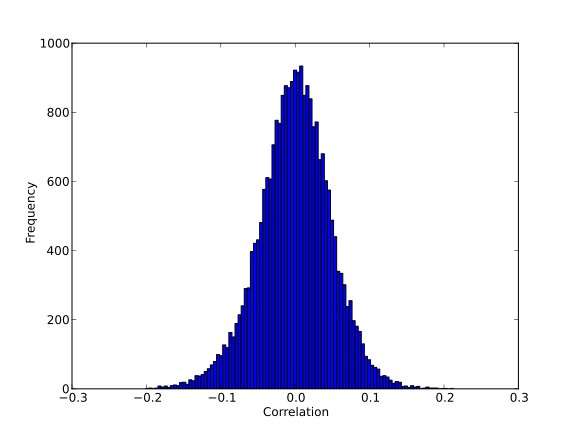
\includegraphics[width = 0.8 \columnwidth]{backchannel/correlationHist.pdf}

\caption[Histogram of correlation for corresponding algorithmic geometric features that originate from \textit{different} conversations.]{Histogram of correlation for corresponding algorithmic geometric features that originate from \textit{different} conversations. The standard deviation is 0.048 and the variance is 0.002.}
\label{FigureCorrelationHist}
\end{figure}

The statistical significance of the best correlated features can be confirmed by characterising the distribution of correlation performance scores for the null hypothesis and use it to calculate the p-value for the hypothesis of interest. The possibility of a null hypothesis can be discounted if this p-value is lower than the desired significance level $\alpha$ and can then be considered as statistically significant (see Hayes \cite{Hayes2005}). Because multiple hypothesises are tested, $\alpha$ is adjusted using the Bonferroni correction to account for the greater chance of finding coincidental patterns. Any correlations between feature pairs that originate from separate conversations are due to chance. The distribution of correlation scores for null hypothesis pairings is shown in Figure \ref{FigureCorrelationHist}. The standard deviation of correlation scores from null hypothesis pairings is $\sigma=0.048$ and the variance is $\sigma^2=0.002$. The chance correlation distribution is zero centred $\bar{\correlFunc}=0$. The p-value of a correlation score $\correlFunc$ is calculated by a z-test. A z-test is used because the standard deviation of all possible null hypothesis is known. For a single observation compared to a zero centred population $\bar{\correlFunc}=0$, the z-test score is defined as:

\begin{gather}
z = \frac{\correlFunc}{\sigma}
\end{gather}

For the highest correlation by chance, $\correlFunc=0.21$, the corresponding z-score is $z=-0.21/0.048=−4.4$ and p-value is $2\times\mathcal{N}(−4.4)=1.2\times10^{-5}$ where $\mathcal{N}$ is the cumulative normal distribution. The double tailed score is used because the modulus of the correlation is used to determine the largest magnitude correlation. The standard significance level $\alpha$ is usually chosen to be either $0.01$ or $0.05$. The more stringent level $\alpha=0.01$ is used in this chapter. Each of the correlation scores use the maximum value, based on 1035 comparisons (see Section \ref{SectionGenerateAlgorithmic}). The Bonferroni corrected $\alpha$ is calculated as $\alpha_{adjusted} = \frac{0.01}{1035}=9.7\times10^{-6}$. The p-value of $1.2\times10^{-5}$, observed in the validation experiments, is within this threshold and cannot be considered as a statistically significant finding, as should be expected. 

For pairings in which are engaged in the same conversation, patterns that are clearly statistically significant are expected. The correlation scores for these conversations vary from $\correlFunc=0.25$ to $\correlFunc=0.38$. This corresponds to p-values between $2\times\mathcal{N}(-0.25/0.048)=1.9\times10^{-7}$ and $2\times\mathcal{N}(-0.38/0.048)=2.4\times10^{-15}$, respectively. These are well below the Bonferroni corrected significance level of $9.7\times10^{-6}$. The null hypothesis may therefore be rejected for these tests and they are therefore statistically significant.

\begin{figure}[tb]
\centering
\includegraphics[width = 0.49 \columnwidth]{backchannel/1008.pdf}
\includegraphics[width = 0.49 \columnwidth]{backchannel/1011.pdf}

\includegraphics[width = 0.49 \columnwidth]{backchannel/3008.pdf}
\includegraphics[width = 0.49 \columnwidth]{backchannel/3011.pdf}
\caption[Corresponding facial distances found to be most coupled in natural conversation for two of the conversations, marked in green.]{Corresponding facial distances found to be most coupled in natural conversation for two of the conversations, marked in green. The top row is conversation 1008-1011. The bottom row is conversation 3008-3011.}
\label{BackChannelCoupledPose}
\end{figure}

\begin{figure}[tb]
\centering
\includegraphics[width = 0.49 \columnwidth]{backchannel/2008.pdf}
\includegraphics[width = 0.49 \columnwidth]{backchannel/2011.pdf}

\includegraphics[width = 0.49 \columnwidth]{backchannel/6008.pdf}
\includegraphics[width = 0.49 \columnwidth]{backchannel/6011.pdf}
\caption[Corresponding facial distances found to be most coupled in natural conversation for two of the conversations, marked in green.]{Corresponding facial distances found to be most coupled in natural conversation for two of the conversations, marked in green. The top row is conversation 2008-2011. The bottom row is conversation 6008-6011.}
\label{BackChannelCoupledMouth}
\end{figure}

The two areas of the face found to be coupled in natural conversation are shown in Figures \ref{BackChannelCoupledPose} and \ref{BackChannelCoupledMouth}. The areas shown in Figure \ref{BackChannelCoupledPose} seem to involve vertical distances which are generally rigid and likely encode head pitch. In contrast, the second group's relevant areas, shown in Figure \ref{BackChannelCoupledMouth}, are more related to the mouth and perhaps relate to mutual smiling or some other mouth related expression.
%1011,1008,0.248663511096,886,886 10045-488 P
%2011,2008,0.384282031869,903,903 10119-488 M
%3011,3008,0.343704739655,230,230 6249-1924 P
%6011,6008,0.375698211625,661,661 6718-488 M
The next section attempts to find patterns in facial behaviour that are not necessarily related to corresponding areas of the face.

\subsection{Coupling of Shape for Non-corresponding Facial Features}

\begin{table}[tb]
\centering
\caption[Maximum correlation $\dyadicCorrelation_{max}$ of \textbf{facial shape features} for different pairs of participants (including corresponding and non-corresponding features).]{Maximum correlation $\dyadicCorrelation_{max}$ of \textbf{facial shape features} for different pairs of participants (including corresponding and non-corresponding features). Pairs that were participating in the same conversation are highlighted.}
\begin{tabular}{ | c | c | c | c | c | c | c | c | c |}
\hline
& 1008 & 1011 & 2008 & 2011 & 3008 & 3011 & 6008 & 6011 \\
\hline
1008 & \cellcolor{orange} 1.00 & \cellcolor{orange} 0.30 & 0.18 & 0.15 & 0.23 & 0.22 & 0.15 & 0.18\\
1011 & \cellcolor{orange} & \cellcolor{orange} 1.00& 0.25& 0.22& 0.29& 0.23& 0.21& 0.23\\
2008 & & & \cellcolor{orange} 1.00& \cellcolor{orange} 0.43& 0.17& 0.23& 0.17& 0.18\\
2011 & & & \cellcolor{orange} & \cellcolor{orange} 1.00 & 0.22& 0.19&0.18 &0.19 \\
3008 & & & & & \cellcolor{orange} 1.00 & \cellcolor{orange} 0.49& 0.18& 0.29\\
3011 & & & & & \cellcolor{orange} & \cellcolor{orange} 1.00& 0.21& 0.16\\
6008 & & & & & & & \cellcolor{orange} 1.00& \cellcolor{orange} 0.42\\
6011 & & & & & & & \cellcolor{orange} & \cellcolor{orange} 1.00\\
\hline
\end{tabular}
\label{TableBackchannelShape}
\end{table}

The previous section considered the interpersonal coordination of facial behaviour for corresponding areas of the face. However, facial behaviour coupling between people may be expressed in different facial areas. This falls within the definition of synchrony, for which ``the important element is the timing, rather than the nature of the behaviours'' \cite{Delaherche2012}. Synchrony can involve coordinated times of different forms of behaviour, e.g. beginning to speak when another person stops speaking. This phenomena has been explored to some extent by Ramseyer and Tschacher \cite{Ramseyer2008}, who did not use corresponding parts of the body but instead searched entire images for any movement synchrony. To find correlations for this broader problem, the feature component $i$ for subject $A$ is compared to feature component $j$ for subject $B$. Because each feature component corresponds to a different area of the face, this searches for relationships in shape between non-corresponding facial areas. The correlation between facial components $i$ and $j$ ($i \in \{0...\numFeatures\}$ and $j \in \{0...\numFeatures\}$) defined as $\dyadicCorrelation^{A,B}_{i,j} \in \mathbb{R}$ for subject $A$ and $B$:

\begin{gather}
\dyadicCorrelation^{A,B}_{i,j} = \correlFunc(\frameFeatureMatrix^A_i, \frameFeatureMatrix^B_j) \\
(i_{max}, j_{max}) = \argmax_{i,j}{\dyadicCorrelation^{A,B}_{i,j}}
\end{gather}

Again, the components $i_{max}, j_{max}$ with the highest correlation $\dyadicCorrelation^{A,B}_{i,j}$ are determined. The result of this process is shown in Table \ref{TableBackchannelShape}. The correlation for pairs in the same conversation is consistently above the correlation of coincidence matches. The standard deviation of correlation scores from null hypothesis pairings is $0.047$ and the variance is $\sigma^2=0.002$, which is similar to the case of chance correlations if only corresponding features are considered (see Figure \ref{FigureCorrelationHist}). More comparisons are performed to obtain the maximum correlation for each pair of subjects. This results in a more stringent Bonferroni adjusted $\alpha$, which is calculated as $\alpha_{adjusted} = \frac{0.01}{T_{1035-1}}=1.87\times10^{-8}$ where $T_i$ is the $i$th triangular number. For pairs of subjects in engaged in conversation, the maximum correlation for each pair is 0.30, 0.43, 0.49 and 0.42. Based on the z-test, these correlations have a p-value of $1.7\times10^{-10}$, $5.75\times10^{-20}$, $1.90\times10^{-25}$ and $4.03\times10^{-19}$ respectively. The first is relatively near the significance boundary, while the latter three results are clearly statistically significant. There may be because the broader range of facial areas considered includes a wider range of human expression, so instead of just co-occurrence behaviours, other strongly coupled communication relationships can be detected. Because a greater number of feature components are compared, there is an increased possibility for coincidental matches. This is evident in the table because the off axis pairings show an increase in correlation compared to Table \ref{TableBackchannelShapePairs}. These results indicate that some facial behaviour is coupled and this coupling is stronger if non-corresponding facial areas are also considered. Although the correlation scores are above chance occurrence, they are not perfectly consistent patterns of human behaviour. This does not make this patterns uninteresting or insignificant because most inter-personal behaviours are only general patterns; identification of deterministic patterns in human behaviour are not the norm.

%So far in this chapter, coupling of face deformation has been investigated. The next section considers behaviour coupling based on variation of face shape in a sliding window.

\subsection{Coupling of Facial Shape Activity for Non-corresponding Facial Features}

\begin{table}[tb]
\centering
\caption[Maximum correlation $\dyadicCorrelation_{max}$ of sliding window \textbf{variance of facial shape}, for various pairs of participants (including corresponding and non-corresponding features).]{Maximum correlation $\dyadicCorrelation_{max}$ of sliding window \textbf{variance of facial shape}, for various pairs of participants (including corresponding and non-corresponding features). Pairs that were participating in the same conversation are highlighted.}
\begin{tabular}{ | c | c | c | c | c | c | c | c | c |}
\hline
& 1008 & 1011 & 2008 & 2011 & 3008 & 3011 & 6008 & 6011 \\
\hline
1008 & \cellcolor{orange} 1.00& \cellcolor{orange} 0.32& 0.13& 0.13& 0.29& 0.38& 0.16& 0.27\\
1011 & \cellcolor{orange} & \cellcolor{orange}1.00& 0.33& 0.21& 0.19& 0.16& 0.21& 0.18\\
2008 & & & \cellcolor{orange} 1.00& \cellcolor{orange}0.34& 0.11& 0.23&0.16 &0.21 \\
2011 & & & \cellcolor{orange} & \cellcolor{orange}1.00 & 0.12& 0.14& 0.26& 0.29\\
3008 & & & & & \cellcolor{orange}1.00& \cellcolor{orange}0.41& 0.47& 0.14\\
3011 & & & & & \cellcolor{orange} & \cellcolor{orange}1.00& 0.27& 0.25\\
6008 & & & & & & & \cellcolor{orange}1.00&\cellcolor{orange} 0.15\\
6011 & & & & & & & \cellcolor{orange} & \cellcolor{orange}1.00\\
\hline
\end{tabular}
\label{TableBackchannelVar}
\end{table}

The previous sections have examined coupling of face shape in natural, dyadic conversation. However, it may be that facial motion contains reliable patterns of human behaviour. For instance, head pitch activity might encode nodding in agreement and this may be related to mouth activity caused by talking. The variance of each feature component in a sliding window was calculated. The window was selected to be 1 second in duration (25 frames), because this is sensitive to \ac{NVC} signals of a relatively short duration. However, different \ac{NVC} signals may occur on other time scales which would not be detected. At sliding window position $\timeOffset$, the variance $\slidingWindowVar$ of a feature component in a sliding window of 25 frames duration is:

\begin{gather}
\label{EqnVarianceSlidingWindow}
\slidingWindowVar^A_{\timeOffset,i} = \frac{1}{25} \displaystyle\sum\limits^{12}_{a=-12} {\frameFeatureMatrix^A_{\timeOffset+a,i}}^2 - \left( \frac{1}{25}\displaystyle\sum\limits^{12}_{a=-12} {\frameFeatureMatrix^A_{\timeOffset+a,i}} \right)^2\\
\dyadicCorrelation^{A,B}_{i,j} = \correlFunc(\slidingWindowVar^A_i, \slidingWindowVar^B_j)
\end{gather}

The results of this method are shown in Figure \ref{TableBackchannelVar}. In this case, the correlations caused by coincidence (shown in the off axis pairings) are often higher than the correlations that might be expected to have coupling. The variance of correlations from null hypothesis pairings has a standard deviation of $0.034$. For subject pairs engaged in conversation, the maximum correlations were 0.32, 0.34, 0.41 and 0.15. Based on the z-test, the p-values for these results are $4.88\times10^{-21}$, $1.52\times10^{-23}$, $1.74\times10^{-33}$ and $1.03\times10^{-05}$ respectively. The first three pairings are well below the significance threshold $\alpha_{adjusted} = \frac{0.01}{T_{1035-1}}=1.87\times10^{-8}$ but the final pair is above the threshold and is more likely to be due to a null hypothesis. The highest correlation is for conversation 3008-6008 which has $\dyadicCorrelation=0.47$ and is caused by coincidental variation of the features (p-value $1.84\times10^{-43}$). This coincidental match is strangely below the significance threshold and may be due to the distribution of correlations being non-Gaussian. Since coupling cause by patterns in human behaviour cannot be distinguished from those cause by coincidence, more data is required to obtain results that can be confidently considered as statistically significant. An analysis of facial shape activity based on corresponding features resulted in a similar, non-significant result and has been omitted for brevity. This system was not compared to human performance for identifying interpersonal coordination because the resources required to collect such an annotation data set would be very resource intensive and this is beyond the scope of this thesis.
Facial shape in natural conversations exhibits interpersonal coordination. Given the relationship between people's behaviours, the next section uses backchannel information for automatic \ac{NVC} recognition. However, the following section considers all feature components rather than the components identified in earlier in the chapter. This allows features to be used in the classifier model that do not necessarily have a linear coupling with the forward channel behaviour.

\section{Classification Based on Backchannel Information}
\label{SectionClassificationBackchannel}

The previous chapter has investigated automatic methods to classify \ac{NVC} based on visual facial information. However, the corpus has two subjects interacting. The annotated subject is designated as the ``sender'' and the other conversation participant as the ``receiver''. 
The sender expresses in the forward channel and perceives the backchannel. The receiver expresses in the backchannel and perceives the forward channel. 
The previous section has discussed coupling of facial behaviour in natural conversation. This raises the possibility that a sender's \ac{NVC} signals may be inferred based on the receiver's visual information. Figure \ref{BackChannelFigure} shows the experimental arrangement to detect \ac{NVC} using backchannel signals. The videos of \ac{NVC} receiver participants are tracked and features extracted using \textit{geometric-a} features, as described in Section \ref{SectionGenerateAlgorithmic}. A classifier is trained on the sender \ac{NVC} labels and the receiver facial feature data. Testing is performed on a person independent basis, with only clear \ac{NVC} clips used in the test $\clearClipSet^{clear}_{\nvcCategory}$ (see Section \ref{SectionClearExamples}) based on annotation ratings of the \ac{NVC} sender. %Test features are used to train an \ac{SVM} classifier.

\begin{figure}[tb]
\centering
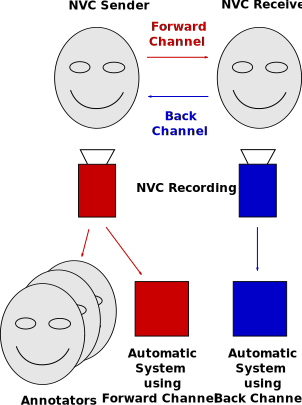
\includegraphics[width = 0.4 \columnwidth]{backchannel/figureforwardbackchannel.pdf}
\caption{Automatic \ac{NVC} classification can operate on either the forward or backchannel information.}
\label{BackChannelFigure}
\end{figure}

The experimental arrangement is almost identical to that presented in the previous chapter. The target classes and annotation data is described in Chapter \ref{ChapterCorpus}. \FeatureGeneration is performed as discussed in Section \ref{SectionFeatureGeneration}. Classification is performed as described in Section \ref{SectionClassificationMethods}. Eight fold cross validation is used on clear examples of \ac{NVC} (Section \ref{SectionClearExamples}) and performance is evaluated using \ac{AUC}, as described in Section \ref{SectionClassificationPerformance}. The only difference is the shape features used for training and testing are taken from the other person in the dyad (i.e. the person conversing with the subject that was shown to the annotators).

\subsection{Results and Discussion}

\thesisstatement{Classification of NVC is possible from backchannel signals but is more difficult than forward channel.}

\thesisstatement{Algorithmic features are good at generalising to the person independent NVC classification and regression (for forward and backchannel signals)}

The performance of automatic classification based on backchannel \ac{NVC} signals is shown in Table \ref{TableBackchannel}. If the performance for forward channel \ac{NVC} classification (Table \ref{TableCompareFeaturesAndClassifiers}) is compared to backchannel performance, it can be seen that the backchannel performance is equal or lower in every case. This is unsurprising, because backchannel information is only a behavioural response to forward channel communication. The results suggest that, for some methods of \featureGenerationComma the classifier is consistently performing at above chance level of 0.5. However, additional tests are required to establish if this result is statistically significant. If the performance for each of the \featureGeneration methods is compared, it can be seen that \textit{geometric-a} features are again the most effective. The majority of other feature sets have performance levels at or near chance level. Person independent testing is more challenging than multi-person testing in all cases. 
%The best performing features are geometric based with \textit{geometric-h} has a larger drop moving from multi-person to person independent. 
These observations have the same general pattern as the forward channel performance results.

\begin{table}[tb] % XIV, XII, XV, XIII
\centering
%\rowcolors[]{1}{white!20}{white!10} 
\caption{\ac{AUC} \ac{ROC} performance using backchannel features (clip level testing, person independent testing, average score of categories and average standard deviation from Tables \ref{BoostClipMultipersonReceiverTable} to \ref{SvmClipPersonindepReceiverTable} are shown).}
\begin{tabular}{ c | c | c | c | c }
\hline
Test & \multicolumn{2}{c|}{Multi-person} & \multicolumn{2}{c}{Person independent} \\
 & SVM & Adaboost & SVM & Adaboost \\
\hline
affine                           & 0.50 $\pm$ 0.04 & 0.53 $\pm$ 0.05 & 0.49 $\pm$ 0.05 & 0.50 $\pm$ 0.04 \\
deform-cubica                    & 0.51 $\pm$ 0.01 & 0.52 $\pm$ 0.05 & 0.50 $\pm$ 0.00 & 0.49 $\pm$ 0.06 \\
deform-fastica                   & 0.51 $\pm$ 0.01 & 0.52 $\pm$ 0.05 & 0.50 $\pm$ 0.00 & 0.49 $\pm$ 0.06 \\
deform-pca                       & 0.54 $\pm$ 0.04 & 0.62 $\pm$ 0.07 & 0.50 $\pm$ 0.00 & 0.52 $\pm$ 0.04 \\
geometric-h                      & 0.65 $\pm$ 0.05 & 0.66 $\pm$ 0.07 & 0.54 $\pm$ 0.04 & 0.59 $\pm$ 0.07 \\
\rowcolor[gray]{.95} geometric-a & 0.67 $\pm$ 0.03 & 0.68 $\pm$ 0.09 & 0.59 $\pm$ 0.08 & 0.59 $\pm$ 0.09 \\
lbp                              & 0.54 $\pm$ 0.05 & 0.58 $\pm$ 0.05 & 0.49 $\pm$ 0.07 & 0.48 $\pm$ 0.10 \\
lm                               & 0.55 $\pm$ 0.03 & 0.56 $\pm$ 0.06 & 0.48 $\pm$ 0.02 & 0.50 $\pm$ 0.05 \\
\hline
\end{tabular}
\label{TableBackchannel}
\end{table}

One difference between backchannel and forward channel is that \ac{SVM} classification has equal to or worse performance when compared to Adaboost. This may be due to over fitting of the SVM, which might be addressed by parameter tuning.

%The next section draws general conclusions based on the chapter's results.

\section{Conclusion}

This chapter has identified coupled behaviour in facial expression and described a study of backchannel features to classify forward channel \ac{NVC}. This was based on previous research that found many human behaviours are inter-personally coordinated in two person conversations. Coupled facial deformations were identified for both corresponding regions of the face, as well as non-corresponding regions. The corresponding areas are situated in the mouth area or were thought to relate to head pitch. Classification was also possible using backchannel features, although the performance is significantly lower if compared to forward channel features. 

This area of research is still at an early stage. There are many potential improvements and extensions to the work presented in this chapter. For instance, coupled behaviours were only examined in conversation pairs, which may lead to personal differences in behavioural patterns. It would be possible to modify the method to look for behavioural patterns that consistently occur across a larger group of conversation participants. Also, only instantaneous face deformations were considered. If an effective way of encoding face deformation or gesture was found, it may be possible to check for responses to stimuli that occur after a time delay, in a similar fashion to Richardson \etal \cite{Richardson2007}. Pearson's correlation coefficient is only sensitive to linear correlations between variables, but it is quite possible that non-linear behavioural patters may exist. Only facial deformation is considered in the features and it would be interesting to expand the behavioural encoding to verbal communication, as well as arm position and body pose. This would enable a much broader range of social phenomena to be studied.

There are also possible extensions to classification based on backchannel features. It should be possible to combine backchannel and forward channel features, either by feature or decision fusion, to improve performance. Also, many of the limitations of the previous chapter apply here: \ac{NVC} is not temporally modelled, and the social context and cultural background of the participants and annotators could be better controlled. To address the cultural differences of the annotators, the next section describes the collection of a \culturallySpecific annotation set for the TwoTalk corpus.



\begin{savequote}
There is no truth. There is only perception.
\qauthor{Gustave Flaubert}
\end{savequote}

\chapter[Multiple Culture Annotation]{Multiple Culture Annotation}
\label{ChapterAnnotation}

\thesiscomment{MAIN POINT: Because cultural perception differences are expected to exist, we collect a new cross culture annotation set using crowdsourcing and address the filtering issues to produce three distinct annotation sets that reflect individual annotator's ratings.}

\thesiscomment{WHAT we do}

\thesiscomment{HOW we do it}

\thesiscomment{RESULTS, IMPACT and NOVELTY}

\thesiscomment{Of course, we expect to find cultural differences. Make it clear why this work is necessary despite that.}

%The previous two chapters describe an automatic system that attempts to recognises \ac{NVC} as humans would rate the same signal. 
Humans often disagree as to the meaning that is expressed in a video clip of \ac{NVC}. As discussed in Section \ref{SectionAnalysisOfMeanRatings}, the statistical mean of ratings is used to form a single label for each video clip. If there is significant inter-annotator disagreement in the data, taking the mean is not necessarily valid because the resulting label does not correspond to any specific human or group of human annotators. One of the factors that affects \ac{NVC} signal perception by humans is the cultural background of the observer (see Section \ref{BackgroundWhatFactorsInfluenceNvc}). As the goal of automatic recognition of \ac{NVC} is to produce labels similar to those generated by humans, modelling the specific cultural perception of \ac{NVC} signals will lead to improvement over training a system in one culture and then applying it in a different culture.% that is not reflected in the training data.
%Using multiple groups of annotations, each which produce an independent subjective set of annotations. 

For the purposes of automatic recognition, all previous research has either gathered annotation data from a specific culture or merged annotations from multiple cultures. This is the first study using subjective annotation for machine learning so that cultures were kept as distinct annotation sets. 
%However, this is not the first to use machine learning on subjective data based on distinct annotators; Reidsma and op den Akker \cite{Reidsma2008b} trained annotator specific classifiers based on contextual addressing labels in a meeting social context.

The main contributions of this chapter are:
\begin{itemize}
 \item Annotation data, based on crowdsourcing, that is suitable basis for automatic recognition of human behaviour.
 \item A quantitative analysis of cross cultural annotation data. The data is analysed in terms of quantifying the possible existence and extent of differences between cultural specific perceptions.
\end{itemize}

Research relating to cultural differences and crowdsourcing are discussed in the next section. Section \ref{SectionCrowdSourceDataCollection} describes the Internet based collection of annotation data. This data is filtered to remove uncooperative workers; the filtering method is described in Section \ref{SectionNeedToFilter}. Section \ref{SectionAnalysisOfCultureAnnotation} describes an analysis of the filtered data.

\section{Related Research}
\label{BackgroundCrossCulture}

The field of cross cultural study of emotion was founded by Darwin in 1872 \cite{Darwin2002}, in which he was struck by the remarkable similarity in emotion expression styles across cultures. 
%The books impact was later assessed by Ekman \cite{Ekman2009}, who claimed that Darwin's key contributions were the emphasis of emotions that were discrete entities that were primarily expressed by the face and had limited universality across cultures and species. 
Darwin also pioneered the use of photographs in the study of emotion, and the assessment of emotion by judgement based studies \cite{Ekman2009}. The key role of culture in non-verbal communication was stressed by Hall \cite{Hall1959}, with particular attention to cultural influences of which the expresser is not consciously aware. Ekman modelled the process of differences in emotion expression by proposing culturally specific display rules \cite{Ekman1969}, but claimed that emotion was largely culturally universal, and this universality was particularly evident in a subset of emotions called ``basic emotions'' \cite{Ekman1972}.
% although he also uses the term ``basic emotions'' for his particular discrete emotion/evolutionary view of emotions \cite{Ekman99}. 
There is less evidence for the universality of non-verbal communication but emotion can be a form of communication \cite{Frith2009}, and that component of \ac{NVC} may be partly universal. %Cultural differences exist in both expression and perception of emotion. Experimental work that examines these differences will now be discussed.

% Possibly relevant? definition of basic emotions? \cite{Ortony1988}, 
Cultural differences in expression of emotion and \ac{NVC} have been studied and observed \cite{Matsumoto2006}. Extreme cases of cultural difference in perception include different head motions for agreement and disagreement \cite{Kassabova2008}, and differences in obscene gestures \cite{Knapp2009}. Gaze aversion direction while thinking has cultural differences \cite{McCarthy2006}. Backchannel signals are more frequent in Japanese culture than \acs{US} culture \cite{White1989}. These differences may be significant for an automatic system if it is trained for one culture and deployed in a different culture. Various cross cultural studies have collected observer judgements and each time have found cultural differences. This has included judgements of pictograms \cite{Cho2007} and emotional avatars \cite{Massaro96, Koda2007}. Marsh \etal found that observers could distinguish a person's nationality by their style of emotional expression \cite{Marsh2003}. Japanese observers were found to be more sensitive to context than Westerners in emotion recognition \cite{Masuda2008}. Some universality was found for non-verbal vocalisation of the common Ekman 6 basic emotions but cultural differences were found in non basic emotions \cite{Sauter2009}. Even the process of perception has been seen to have cultural differences: gaze during emotion recognition were found to have different patterns \cite{Jack2009}, which possibly leads to some cultures having difficulty distinguishing certain emotions. All these findings suggest that differences in expression and perception exist but also there is a great deal of commonality between cultures.

%A cross cultural study linked differences in display rule differences to cultural traits \cite{Matsumoto08}

Elfenbein and Ambady \cite{Elfenbein2002b, Elfenbein2002} argued that members of a cultural group are more accurate at recognising emotions in their group, when compared to an out-of-group observer. In response to this paper, Matsumoto argued that for the group hypothesis to be properly tested, the sample sizes needed to be balanced and the stimuli had to be equivalent \cite{Matsumoto2006} and this had not been done. The potential for culturally specific concepts can make \ac{NVC} and emotion words difficult to translate or transfer to new cultures (see Section \ref{SectionTranslationOfInstrument}). If an in-group advantage exists for \ac{NVC}, cultures that differ from the expresser's culture may annotate data differently. This may range from a reduction in inter-annotator agreement to significant misinterpretations of the \ac{NVC} meaning. %While there have been a vast number of cross cultural studies of human behaviour, none have been used as a basis for machine learning of human behaviour recognition.
% This may be that certain concepts are only meaningful within a culture (an ``emic'' account), which contrasts with an observer outside a culture that (an ``etic'' account) \cite{Headland1990}.

Various approaches exist to detect and remove outliers in questionnaire responses \cite{Zijlstra2011}. The method proposed in this chapter differs in that it considers each annotator response set as something to be accepted or rejected as an entirety. This property makes it more suitable to a crowdsourcing application.

%DISCUSS? Inter-annotator disagreements imply bad automatic results? \cite{Reidsma2008Thesis}

\subsection{Crowdsourcing of Annotation Data}

Crowdsourcing refers to the participation of a loosely defined group of people who work towards a common goal, often using the Internet to coordinate the work. Some scientific projects have used crowdsourcing and involving many workers from across the world, including Cooper \etal \cite{Cooper2010}, for ``foldit'' protein folding and Riddick \etal for ``Galaxy Zoo'' \cite{Raddick2010} which generated enough interest to not need payment to incentivise participation. Tarasov \etal \cite{Tarasov2010} proposed using crowdsourcing to gather emotional label annotation data. There are few or no previous works that use crowdsourcing for annotation of \ac{NVC} behaviour, for the purposes of automatic recognition. The next section describes how crowdsourcing was applied to annotation of \ac{NVC} samples.

\section{Data Collection Method}
\label{SectionCrowdSourceDataCollection}

The annotation task involves viewing a series of short views from the corpus (as described in Section \ref{SectionDescriptionOfTwoTalkCorpus}) and providing responses to the questions on \ac{NVC} signals (described in Section \ref{SectionDescribeQuestions}). Computer based annotation is commonly used for annotation because the annotation task can be precisely defined by the experimenter, and because of the convenience of collection and analysis of the results. Computer based annotation may also be conducted remotely, which is cost effective and convenient but provides less control on how the annotators complete the task. Differences in the equipment, the presence or absence of audio and a different physical environment may affect how an annotator perceives an \ac{NVC} signal. These factors could not be controlled using remote computer based annotation and may result in an increase of inter-annotator differences.

%Some tasks are sufficiently interesting as to not require a monetary incentive for annotators to participate. However, given our annotation task is relatively arduous (see Section \ref{BackgroundWhyNvcAnnotationIsBoring}), Internet crowdsourced workers were used and were paid a small fee to complete each annotation task. 
The annotation data was collected from multiple cultures.
Crowdsourced workers may be located anywhere in the world and they use any standards compliant web browser to complete tasks which have been defined by a work supplier. There is usually little screening of workers and no qualification or requirements beyond being able to access the Internet. A typical screen shot of the web page presented to the annotator is shown in Figure \ref{FigureAnnotationSurveyScreenshot}. Although it is quite possible to independently establish a website that enables annotation and payments, there are several web-based services that manage the website infrastructure for a fee. Crowdflower's web service\footnote{\scriptsize{http://crowdflower.com/}} was used to manage the annotation work. This service provides a high level interface to other crowdsourcing services, such as Amazon Mechanical Turk\footnote{\scriptsize{https://www.mturk.com/}} and Samasource\footnote{\scriptsize{http://samasource.org/}}. Each service has an associated worker pool with a distinct worker demographic. However, crowdsourcing has several issues that need consideration if high quality annotation is required.

As previously mentioned, the order of the questions presented to the annotators was randomised to reduce the effect of question order. It was impossible to insert a demographic survey before the users undertook the main task. This was unfortunate, because demographic information may be useful in accounting for inter-annotator differences. However, the IP address of each annotator was available, which was used to assign a rough geographic location of each Internet user. Also, Samasource specialises in refugee populations and an annotators physical location can differ from their cultural background. In particular, a significant response was received from annotators located in Kenya, but these people were likely to be Sudanese refugees. Also, an IP address is not a perfectly reliable method to localise users, given the existence of Internet proxy services. Despite these factors, an IP address based location was considered sufficient for our needs. In the case of refugees, it is not necessary to know the exact culture of origin, as long as the IP address location corresponds to multiple distinct cultural groups. 

Volunteers may be sampled from a sub-group within each culture and this effect is called ``sampling bias''. 
%Computer based tools are used to perform the annotation. 
The availability of skills and equipment varies in each population, therefore if computer use is required, sample bias is likely to occur. The extent of this bias is unknown. It is possible that there is no unified \ac{NVC} perception consensus in a single culture, if any intra-culture factor has a large effect on \ac{NVC} perception. It may therefore be undesirable to sample from an entire country's population, if the annotations within a group are not in agreement. However, using a sub-group of a culture is satisfactory, as long as the sample is not assumed to represent the culture as a whole. If the applications of this technology are to be adopted by a sub-group of a culture, such as those with easy access to computers, this bias may be beneficial in creating a system that operates well with potential users. In conventional surveys, various techniques can be used to improve annotator agreement, such as training, annotators previewing the corpus, panel-based ratings, repeat ratings of a clip by the same annotator. These were not used because of the technical limitations of the present crowd sourcing tools, for which work unit presentation is pseudo-random. Annotator normalisation was not used because the annotation data is sparse and  perception labels of individual annotators is not required for this study, but this technique may be adapted to this situation in future work.

The survey data described in Section \ref{SectionAnalysisOfHumanAnnotation} was collected using unpaid volunteers. This chapter relies on paid workers to provide annotation data. Given that it was possible for an annotator to provide random data in return for a monetary reward, there can be quality control issues which need to be managed. The process for filtering valid work from random annotation is described in Section \ref{SectionNeedToFilter}. The workers that accept to complete the task as instructed are designated as ``trusted'' workers, and annotators that respond with poor data or random data are designated as ``untrusted''. Crowdflower provides its own semi-automatic tool for identifying trusted workers called ``gold'', presumably from the term ``gold standard''. This gold tool was used to reduce expenditure on poor annotation data. However, this tool did not affect the final annotation data and both trusted and untrusted data was retained and filtered using the method described below.

\thesiscomment{Can a simple test question find random responders? Is this better than filtering?}

An alternative approach to identification of trusted workers is to introduce additional validation questions with a known answer. Unfortunately, there are several practical problems with this approach in a crowdsourcing environment. Additional questions increase the amount of work required of the annotators. Due to the current technical limitations of the annotation service, each annotation task or ``work unit'' must have the same number of responses for every question. The basic work unit requires the four \ac{NVC} signal ratings of the questionnaire. To add one more question would increase the workload by 25\%. Also, humans that intend to cheat will be able to identify any validation questions and simply answer them correctly, while randomly answering the \ac{NVC} questions. This possibility of circumventing the validation questions makes their usefulness questionable. The annotation data would still need to be analysed and filtered to provide confidence that the annotation data is valid. The next section discusses the issue of language in the context of \ac{NVC} signal perception ratings.

\subsection{Translation of Cross Cultural Instruments}
\label{SectionTranslationOfInstrument}

The design of the questionnaire was previously discussed in Section \ref{SectionDescribeQuestions} but previously only a single culture and a single language have been considered. 
Different languages are spoken throughout the world with English being the first language for approximately 380 million people \cite{Economist2001}. Second language speakers and learners of English outnumber first language users but the majority of people speak languages other than English. 
The questionnaire was applied to cultures that have significant differences, including language usage. The translation of survey instruments is used in many scientific fields to avoid the instrument being understood differently outside of its original culture. According to Geisinger \cite{Geisinger1994}, an instrument needs to be translated and the fact that the translated instrument measures the same constructs as the original version needs to be verified. A translation may lead to the instrument measuring something other than what was intended \cite{Poyatos1997}, and this makes comparison between cultures problematic. Translation of survey instruments is strongly recommended in medical surveys, using rigorous methods \cite{Gjersing2010, Beaton2000, Morales2001}. Medical surveys contain questions that refer to concepts that are labels for observable phenomena that exist separately from the observer. However, the \ac{NVC} questionnaire is quite different in that the concepts do not exist except as subjective interpretations. The questionnaire asks for an annotator's interpretation of \ac{NVC} signals which depends on their cultural background, etc. The term ``\ac{NVC}'' implies that these communication signals do not directly correspond to word based concepts. De Mendoza \cite{Mendoza2008} argues emotion labels used to express subjective interpretations are not ``defined by necessary and sufficient features'' but rather ``probabilistic concepts with an internal structure with better and worse examples of the category and fuzzy boundaries''. In this view, a particular instance of an emotion might be perceived as mostly agreeing, somewhat blaming, slightly surprised or any other combination of fuzzy overlapping labels. The same can be said of \ac{NVC} signal perception, in that the labels used in the questionnaire are interrelated, fuzzy, partly overlapping and not comprehensive.

% Fernandez-Dols2003 discusses affect to get away from the realism/nominalism problem
% \cite{Davaninezhad2009}
% Translation of survey \cite{Ekman1969} \cite{Haralick1989} \cite{Headland1990} \cite{Marin1991} \cite{Humphrey1993} \cite{Geisinger1994} \cite{Poyatos1997} \cite{Morales2001} \cite{Economist2001} \cite{Fernandez-Dols2003} \cite{Thirumalai2003} \cite{Matsumoto2006} \cite{Cho2007} \cite{Mendoza2008} \cite{Davaninezhad2009} \cite{Gjersing2010} \cite{Noproblem}

Given that an instrument is to be used in multiple cultures, the concepts referred to in the instrument should be consistently understood. There are two approaches that were considered: translating a questionnaire to cultures of interest or to present a single questionnaire in multiple cultures. These approaches will now be discussed in more detail.

If the concepts referred to exist only in the mind of an observer, these concepts might be ``cultural concepts'' that do not necessarily exist in another language or culture. Because no one-to-one mapping exists between different cultural concepts, the translation of instruments and cross culture recognition are problematic \cite{Elfenbein2002}. There are many examples of emotional concepts that do not have direct translations (\textit{verg\"{u}enza} from Spanish to English, \textit{shimcheong} from Korean to English \cite{Mendoza2008}). Applying this to \ac{NVC}, a particular communication action may be perceived in Spain as a particular combination of cultural concepts but in the United Kingdom, a different combination of cultural concepts. With this culturally specific mapping between concept labels and experiences, a perfect one-to-one mapping will be impossible. Therefore, cultural differences could be caused by imperfect translation leading to different cultural concepts used by the annotators or the way emotions are mapped onto the cultural concepts, with no easy way to distinguish these two effects. 

The other approach is to present the same questionnaire in multiple cultures. The words in the questionnaire would be interpreted by the annotators in relation to their own cultural concepts and this can change the basis by which an annotator perceives and evaluates \ac{NVC} signals. %Cultural differences could cause language understanding differences, in turn leading to differences the cultural concepts used by the annotators, or the way emotions are mapped onto the cultural concepts, and as with a translated survey, with no easy way to distinguishing between these two effects.

Given both approaches have problems, the latter option of having a single survey in one language presented to multiple cultures was used. This decision was based on the fact that, given the crowdsourcing tools available at the time, a specific group of annotators could not be targeted by a tailored questionnaire, although this was planned in a future version of the tools. It may be possible to create a questionnaire using word clouds that would lend themselves better to probabilistic translation (e.g. English word cloud to Spanish word cloud). Given all these considerations, the transfer of everyday concepts from one culture to another is complex and a subject worthy of further study. The next section takes the collected annotation data and considers how untrusted annotators can be identified and removed from the data set.

\section{Filtering Untrusted Workers}
\label{SectionNeedToFilter}

\thesisstatement{Internet worker annotation is noisy, but trusted workers can be found by filtering the data}

\begin{figure}
\centering
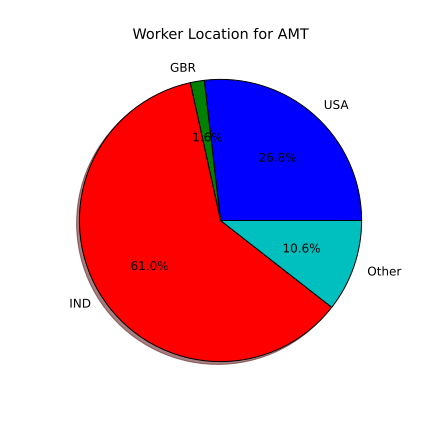
\includegraphics[width = 0.32 \columnwidth]{annotation/demog-amt.pdf}
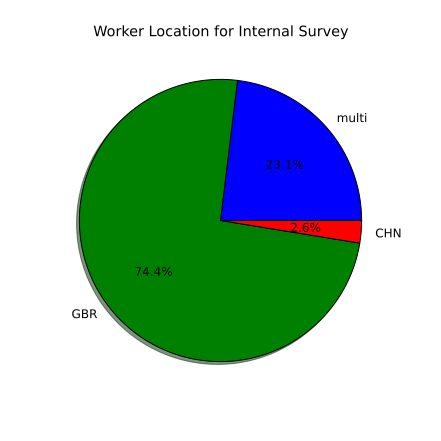
\includegraphics[width = 0.32 \columnwidth]{annotation/demog-internal.pdf}
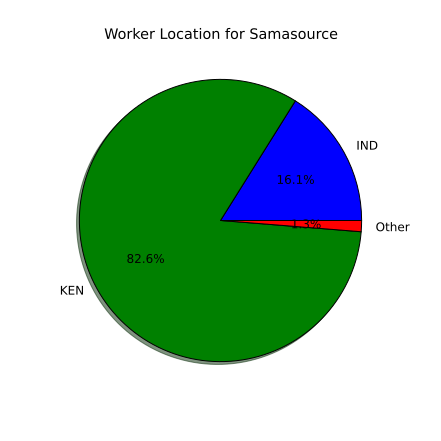
\includegraphics[width = 0.32 \columnwidth]{annotation/demog-sama.pdf}
\caption[Demographics of the worker pools.]{Demographics of the worker pools. AMT is Amazon Mechanical Turk. Each country has been abbreviated to its ISO 3166 code. GBR Great Britain, KEN Kenya, IND India, USA United States of America.}
\label{FigureCrowdDemographics}
\end{figure}

The annotation was performed by 711 participants who provided 79130 individual ratings. These were distributed across 527 video clips and 4 \ac{NVC} categories, with a total of 2108 questions. However, a significant proportion of the data was random, due to a significant proportion of uncooperative annotators. Three distinct worker pools were used. The internal worker pool is primarily the data previously collected and discussed in Section \ref{SectionAnalysisOfHumanAnnotation}, with the inclusion of further annotation by additional volunteers. In all, annotators from 33 countries participated in the annotation task. As can be seen in Figure \ref{FigureCrowdDemographics}, the demographics of each pool differ quite dramatically. Because the annotation data for a single annotator is usually sparse (meaning they are not required to complete every question in the survey), a significant amount of annotation is required for each culture before there is sufficient data to determine stable consensus vote ratings for every question. A considerable amount of annotation data was received from GBR (Great Britain), KEN (Kenya) and IND (India) and these cultures are used throughout the remainder of this thesis. The choice of these cultures is based on the need for distinct cultural groups of any origin, for which annotation data is available. The data from the USA was discarded, along with other cultures with a low level of participation, because the annotators of these cultures did not complete enough questions to form a complete set of results. With better targeting of annotation resources, it would be possible to greatly increase the number of distinct cultures.

The workers were divided into trusted and untrusted groups depending on their cooperation with the task. If the data is not filtered, the resultant labels are extremely noisy and are not appropriate for machine learning. The next section describes the filter method used to ensure the labels are of sufficient quality.

\subsection{Filtering Method}
\label{SectionAnnotationFilterMethod}

\begin{figure}
\centering
\includegraphics[width = 0.3 \columnwidth]{annotation/FlowAnnotationFiltering.pdf}
\caption[Flow chart of filtering method.]{Flow chart of filtering method. The statistical mode rating provides a robust standard by which annotators are assigned a trusted or untrusted score.}
\label{FigureFilterFlowChart}
\end{figure}

%There were three cultures for which a significant amount of data was collected: GBR, IND and KEN. 
Annotators were divided into two groups: trusted and untrusted. To achieve this, each worker's data $\singleAnnotatorRatings_{i, \nvcCategory} \in \mathbb{R}^{\numAnnotators \times 4}$ is compared to a robust rating standard $\robustAnnotation \in \mathbb{R}^{\numClips \times 4 \times 3}$. If a worker correlates with the robust standard to a sufficient degree, they are assigned to the trusted group and if not, the untrusted group (see Figure \ref{FigureFilterFlowChart}). The ratings for a single annotator $i \in \{0...\numAnnotators\}$ is found ($\clipId \in \{1...\numClips\}$):

\begin{gather}
\singleAnnotatorRatings_{i, \nvcCategory} = \{\ratingOfClip_j: (\ratingOfClip_j, \annotatorOfRating_j) \in \rawAnnotation_{\nvcCategory,\clipId}, \annotatorOfRating_j=i\} 
\end{gather}

Annotator $i$ is a member of culture $\textbf{c}_i \in \cultureList = \{GBR, KEN, IND\}$. In this chapter, the raw annotation data $\rawAnnotation$ refers to the cross cultural annotation data. The robust rating standard is based on the statistical mode $\modeFunc$ for clip $\clipId$ ratings, in \ac{NVC} category $\nvcCategory \in \setCategories$, $x \in \cultureList$:

\begin{gather}
\robustAnnotation_{\clipId,\nvcCategory,x} = \modeFunc(\{\ratingOfClip_i: (\ratingOfClip_i, \annotatorOfRating_i) \in \rawAnnotation_{\nvcCategory,\clipId}, \textbf{c}_i = x\})
\end{gather}

\begin{figure}
\centering
\includegraphics[width = 0.6 \columnwidth]{annotation/correlgbr.pdf}
\caption[Histogram of annotator correlation $\rho$ for GBR when compared to the robust ratings $\robustAnnotation$.]{Histogram of annotator correlation $\rho$ for GBR when compared to the robust ratings $\robustAnnotation$. Blue bars indicate annotators above the trusted threshold $\trustedThreshold$, and red bars indicate workers below. The majority of annotators in the GBR group have relatively good agreement with the robust rating.}
\label{FigureCorrelationHistOfGbr}
\end{figure}

\begin{figure}
\centering
\includegraphics[width = 0.6 \columnwidth]{annotation/correlind.pdf}
\caption[Histogram of annotator correlation $\rho$ for IND when compared to the robust ratings $\robustAnnotation$.]{Histogram of annotator correlation $\rho$ for IND when compared to the robust ratings $\robustAnnotation$. Blue bars indicate annotators above the trusted threshold $\trustedThreshold$, and red bars indicate workers below. A significant number of workers in the IND group were assigned to the untrusted group.}
\label{FigureCorrelationHistOfInd}
\end{figure}

\begin{figure}
\centering
\includegraphics[width = 0.6 \columnwidth]{annotation/correlken.pdf}
\caption[Histogram of annotator correlation $\rho$ for KEN when compared to the robust ratings $\robustAnnotation$.]{Histogram of annotator correlation $\rho$ for KEN when compared to the robust ratings $\robustAnnotation$. Blue bars indicate annotators above the trusted threshold $\trustedThreshold$, and red bars indicate workers below. The majority of annotators in the KEN group have relatively good agreement with the robust rating.}
\label{FigureCorrelationHistOfKen}
\end{figure}

The statistical mode is used because it is relatively robust to uniformly distributed noise. Note that the raw annotation $\rawAnnotation$ is usually considered as a interval-scale, dimensional variable but here it is considered as a quantised variable. This is possible because the annotators' responses used a Likert scale with a finite number of options. Histograms of annotator correlation from the three cultures of interest are shown in Figures \ref{FigureCorrelationHistOfGbr}, \ref{FigureCorrelationHistOfInd} and \ref{FigureCorrelationHistOfKen}. As can be seen, there are cultural differences in the proportion of annotators assigned to the trusted and untrusted groups $\workerSet$. IND had a significant proportion of untrusted workers, while GBR and KEN were largely assigned to the trusted group. These perceptual cultural differences are probably more associated with the crowdsourcing worker pools. The vast majority of untrusted workers were in the Amazon Mechanical Turk pool, while annotators from the Samasource and Internal pools were largely trusted. A specific annotator $i$ provided ratings for a set of clips $\clipIndexAnnotated_i$. 
%The ratings $\rawAnnotation_{i}$ for each annotator $i$, having $\numRatingsForAnnotator_i$ across the 4 \ac{NVC} categories, are concatenated to form a combined ratings matrix $\crossCategoryRatings \in \mathbb{R}^{4 \numRatingsForAnnotator_i}$ ($\numRatingsForAnnotator \in \mathbb{N}^{\numAnnotators}$). The combined ratings are $\crossCategoryRatings$ compared to the robust standard $\robustAnnotation$ using Pearson correlation coefficient $\correlFunc$, $i \in \{0...\numAnnotators\}$:
Annotators only usually rate a subset of the corpus. The matrix of ratings by annotator $i$ is designated as $\widehat{\singleAnnotatorRatings}_{i,\nvcCategory} \in \mathbb{R}^{\clipIndexAnnotated_i \times 4}$, and the robust ratings that correspond with this clip subset is designated $\widehat{\robustAnnotation}_{i,\nvcCategory,x} \in \mathbb{R}^{\clipIndexAnnotated_i \times 4 \times 3}$:

\begin{gather}
\widehat{\robustAnnotation}_{i,\nvcCategory,x} = \{\robustAnnotation_{\clipId,\nvcCategory,x}: \clipId \in \clipIndexAnnotated_{i}\} \\
\widehat{\singleAnnotatorRatings}_{i,\nvcCategory} = \{ \singleAnnotatorRatings_{\clipId, \nvcCategory}: \clipId \in \clipIndexAnnotated_{i}\}
\end{gather}

The annotator ratings are then compared to the robust standard using Pearson correlation coefficient $\correlFunc$, $i \in \{0...\numAnnotators\}$. In this case, a 2{D} matrix, element wise Pearson correlation function $\correlFunc'$ to find correlation $\textbf{a}_i \in \mathbb{R}$ is used for convenience:

\begin{gather}
%\hat{\robustAnnotation_i} = {\robustAnnotation_{\nvcCategory,i}: \nvcCategory \in \setCategories}
\textbf{a}_{i} = \correlFunc'(\widehat{\singleAnnotatorRatings},\widehat{\robustAnnotation}_{\textbf{c}_i}) 
\end{gather}

Annotators that have a correlation above threshold $\trustedThreshold \in \mathbb{R}$ are assigned to the trusted set of workers:

\begin{gather}
%i \in \begin{cases}
%\workerSet_{trusted} : a_i \ge \trustedThreshold \\
%\workerSet_{untrusted} : a_i < \trustedThreshold
%\end{cases}
\workerSet_{trusted} = (\workerSet_{all,i} : \textbf{a}_{i} \ge \trustedThreshold) \\
\workerSet_{untrusted} = (\workerSet_{all,i} : \textbf{a}_{i} < \trustedThreshold)
\end{gather}

%If the correlation is above the trusted threshold $\trustedThreshold$, it is included in the set of trusted annotators $\workerSet_{trusted}$. 
A threshold value of $\trustedThreshold = 0.2$ was determined based on the minimum correlation of cooperative annotators from the GBR culture (Figure \ref{FigureCorrelationHistOfGbr}).
The final filtered annotation $\filteredAnnotation$ is computed by taking the statistical mean of trusted annotators. Trusted annotator ratings for a single question form a distribution. The mode only considers the peak of this distribution but disregards the other samples. However, using the mean is more sensitive to the overall views of the annotators. The mean is not a robust measure, which is why it is applied after the data is filtered:

\begin{gather}
\filteredAnnotation^{\clipId, \nvcCategory}_{\cultureSelect} = \overline{\{ \ratingOfClip_i : (\ratingOfClip_i, \annotatorOfRating_i) \in \rawAnnotation^{\clipId}_{\nvcCategory}, i \in \workerSet_{trusted} \}}
\end{gather}

%\begin{table}
%\centering
%\caption{Number of annotators and votes for cultures included in the unfiltered and filtered $\filteredAnnotation$ data set.}
%\begin{tabular}{ | c | c  c | c  c | }
%\hline
%Annotator & \multicolumn{2}{c|}{Num. Annotators} & \multicolumn{2}{c|}{Num. Ratings}  \\
%Country & Unfilter & Filter & Unfilter & Filter \\
%\hline
%\hline
%India & 304 & 167 & 37147 & 22754 \\
%Kenya & 196 & 195 & 15452 & 15420 \\
%GBR & 36 & 26 & 8211 & 8167 \\
%\hline
%\end{tabular}
%\label{NumFilteredWorkersTable}
%\end{table}

\begin{table}
\centering
\caption{Number of annotators and votes for cultures included in the unfiltered and filtered $\filteredAnnotation$ data set.}
\begin{tabular}{ | c || c | c  c || c | c  c | }
\hline
Annotator & \multicolumn{3}{c||}{Num. Annotators} & \multicolumn{3}{c|}{Num. Ratings}  \\
Country & Total & Trusted & Untrusted & Total & Trusted & Untrusted \\
\hline
\hline
India & 304 & 167 (55\%) & 137 & 37147 & 22754 & 14393\\
Kenya & 196 & 195 (99\%) & 1   & 15452 & 15420 & 32\\
GBR   & 36  & 26  (72\%) & 10  & 8211  & 8167  & 44\\
\hline
Total & 536 & 388 (72\%) & 358 (28\%) & 60810 & 46341 & 14469\\

\hline
\end{tabular}
\label{NumFilteredWorkersTable}
\end{table}

where $\cultureSelect \in \cultureList$. The quantity of annotations in the unfiltered $\rawAnnotation$ and filtered $\filteredAnnotation$ annotation sets are shown in Table \ref{NumFilteredWorkersTable}. The 28\% of users that were assigned to the untrusted group accounted for 23\% of the unfiltered data. This implies the trusted annotators answered a greater number of questions on average. After filtering, a significant amount of data remains available for use in training and evaluating machine learning techniques. Each annotator was assigned to a single culture by \ac{IP} address. This information allows a \culturallySpecific robust \ac{NVC} perception rating ($\robustAnnotation_{GBR}$,$\robustAnnotation_{IND}$,$\robustAnnotation_{KEN}$), which are used to filter annotators to form a final, culture specific, filtered annotation sets $\filteredAnnotation^{\clipId, \nvcCategory}_{GBR}$, $\filteredAnnotation^{\clipId, \nvcCategory}_{KEN}$ and $\filteredAnnotation^{\clipId, \nvcCategory}_{IND}$.

\thesiscomment{Is consensus just an artefact of filtering? Hair colour?}

%A method of finding a subset of trusted workers based on their mutual agreement has been described. 
Untrusted annotators were expected to provide uniformly random responses. Filtering the annotators to remove these responses was expected to result in a reduction in variance in the filtered data $\filteredAnnotation$ when compared to the unfiltered data $\rawAnnotation$. There is a possibility that a minority subset of self consistent annotators being selected and this would not represent an overall consensus. However, Table \ref{NumFilteredWorkersTable} shows that the majority of annotators are retained in the trusted set, which shows that this is not the case.

%Given the filtered data $\filteredAnnotation_{GBR}$, $\filteredAnnotation_{KEN}$ and $\filteredAnnotation_{IND}$, cultural differences between the annotators can be analysed. This analysis is performed in the following section.

\section{Analysis of Annotations}
\label{SectionAnalysisOfCultureAnnotation}

The previous section has described how the annotation data was collected from Internet workers and filtering was applied to obtain a high quality set of \ac{NVC} annotations. This annotation data describes the \ac{NVC} content for either \textit{agree}, \textit{thinking}, \textit{question} or \textit{understand} as observed from a particular culture (GBR, KEN or IND). However it is well known that \ac{NVC} perception is dependent on cultural rules and the specifics of cultural factors on \ac{NVC} perception is not well understood. This section provides a quantitative analysis as to the nature and extent of the cultural differences in the annotation data.

\thesisstatement{Annotation of NVC has a low inter-annotator agreement}

\thesisstatement{Different cultures have distinct patterns in their annotation results}

\begin{table}
\centering
\caption{Inter-culture correlation of filtered consensus data for different culture pairs. $\rho_{IND,KEN} = \correlFunc(\filteredAnnotation^{\clipId, \nvcCategory}_{IND},\filteredAnnotation^{\clipId, \nvcCategory}_{KEN})$. Individual annotators are not compared in this calculation but rather the overall cultural consensus.}
\begin{tabular}{ | c | c c c | }
\hline
 & India & Kenya & GBR \\
\hline
\hline
India & 1 & 0.56 & 0.55\\
Kenya &  & 1 & 0.64 \\
GBR    &  &  & 1 \\
\hline
\end{tabular}
\label{InterCultureCorrelationTable}
\end{table}

As can be seen in Table \ref{InterCultureCorrelationTable}, the correlation of pairs of cultures is at an intermediate level. A correlation value of less than one (corresponding to perfect correlation) was expected, because previous studies of emotion have observed cultural differences (see Section \ref{BackgroundCrossCulture}). A Pearson correlation above zero (corresponding to no correlation) implies \ac{NVC} perception in different cultures is not totally independent and a degree of commonality exists. This confirms our suspicion that \ac{NVC} perception is similar to emotion perception in that cultural differences exist, but there remains a significant commonality between cultures. Another point that is illustrated by Table \ref{InterCultureCorrelationTable} is that cultures have varying degrees of similarity to other cultures for perception of \ac{NVC}. The KEN-GBR correlation is higher than either IND-GBR or IND-KEN ($0.64$ vs. $0.56$ or $0.55$). This suggests that IND is the most distinctive in \ac{NVC} perception, and KEN-GBR are relatively similar. It might be expected that other cultures are much more or much less similar than the three cultures studied. This work was restricted to annotators with access to computer and Internet resources, but a broader examination of cultural differences would be interesting.

Pearson's correlation coefficient ignores scaling differences when comparing data. If cultures differed by only scaling differences, this would be ignored by the correlation measure. This is a desirable property, because scaling differences between cultures are relatively trivial to understand and model. However, less than perfect correlation scores indicate that annotation differences exist and they are not merely scaling differences.

\begin{figure}
\centering
\includegraphics[width = 0.78 \columnwidth]{annotation/Sammon3Culture.pdf}
\caption[Sammon mapping of the filtered annotation responses.]{Sammon mapping of the filtered annotation responses. Each point represents the mean rating of a single clip within a single culture. The four \ac{NVC} categories are concatenated into a 4 component vector to enable distance pairs to be computed. GBR: red (.), IND: green (x), KEN: blue (+).}
\label{CultureSammonMapping}
\end{figure}

A way of visualising cultural differences in annotation of \ac{NVC} perception is the Sammon mapping \cite{Sammon1969}. This technique is a dimensionality reduction tool which maps high dimensional samples to a lower dimensional space while preserving inter-sample distances. For culture $\cultureSelect$, the filtered culture annotation $\filteredAnnotation^{\clipId, \nvcCategory}_{\cultureSelect}$ is a $527$ by $4$ matrix. The three filtered cultures  (GBR, IND, KEN) are combined into a $3 \times 527 = 1581$ by $4$ matrix. These points are transformed into a 2{D} space using Sammon mapping and plotted. This allows us to compare the distribution of annotation responses for different cultures. The result of this procedure is shown in Figure \ref{CultureSammonMapping}. This produces a complex distribution with some regions that are generally exclusive to a single culture, areas that are densely occupied by two overlapping cultures and one central zone where all cultures have a high density. The area of three culture overlap corresponds to annotation responses that appear in all cultures, the most common of which likely corresponds to ``no \ac{NVC} is being expressed''. Areas that are dominated by a single culture are interesting because they imply that for a subset of clips, a culture has provided a specific rating for the 4 \ac{NVC} categories that does not appear in the other cultures. This seems to be most apparent in the GBR annotations which has a significant proportion of points that are far from any other culture's points. This supports the idea that cultural differences in \ac{NVC} are not trivial to explain or model, and any mapping between \culturallySpecific annotation sets may be non-linear. 

\thesisstatement{People correlate better with their own culture consensus than with a global consensus}

\thesisstatement{Taking the global mean doesn't correspond to anything in real applications}

\begin{table}
\centering
\caption[Correlation of the mean annotator correlation within various cultures with their respective culture filtered annotation $\filteredAnnotation$ or the global Mean (taken as the combined India, Kenya and \ac{UK} ratings).]{Correlation of the mean annotator correlation within various cultures with their respective culture filtered annotation $\filteredAnnotation$ or the global Mean (taken as the combined India, Kenya and \ac{UK} ratings). Annotators correlate better on average with their own culture consensus than the global consensus $\globalAnnotation$.}
\begin{tabular}{ | c | c c c | }
\hline
 & India & Kenya & \ac{UK} \\
\hline
\hline
Own Culture Mean & 0.67 & 0.78 & 0.77 \\
Global Mean & 0.64 & 0.74 & 0.68 \\
\hline
\end{tabular}
\label{MeanAnnotatorCorrelationTable}
\end{table}

Because various filtering methods and mean ratings are used to arrive at the filtered annotations $\filteredAnnotation$, the extent the filtered annotations are representative of the individual annotator responses should be verified. Also, the validity of disregarding culture and the combining ratings to produce a global mean $\globalAnnotation$ can be considered.
%The filtered annotations is intended to represent the overall culture's \ac{NVC} perception and we should expect a annotator to be more similar to their respective culture, rather than a different culture. TESTS NOT DONE
These comparisons are shown in Table \ref{MeanAnnotatorCorrelationTable} and show an annotator's correlation to their own culture is relatively good. The lower correlation of IND may indicate a problem with data quality or perhaps there is greater perception individuality for this cultural group.
However, if cultural difference is ignored as in the case of global mean annotation $\globalAnnotation$, the individuals do not correlate as well as with their own culture consensus, in all three cases. Therefore, there is a divergence between individual annotators and the ratings that are intended to reflect them. Remember that taking a mean of a group of ratings is only valid if the annotators form a relatively self-consistent group. Therefore, ignoring culture produces a global annotation that has less validity. If global annotation data is used to train an automatic system, the labels that would be predicted would not necessarily correspond to any single annotator or any subset of annotators. This would not be compatible with the objective of producing an automatic system that would predict \ac{NVC} as a human would perceive \ac{NVC}.

\thesiscomment{DISCUSS differences exist other than culture and this is seen here, an area for further work}

\thesiscomment{DISCUSS When does the score converge? about 5 filtered votes?}

\thesiscomment{DISCUSS Any more ideas for analysis? Is there a way to map clusters from different cultures?}

%Conclusions are drawn in the next section, based on the experience of collecting data annotation and the results are analysed.

\subsection{Inter-annotator Agreement}
\label{SectionInterAnnotatorAgreement}

The annotation consensus score $\filteredAnnotation^{\clipId, \nvcCategory}_{\cultureSelect}$ is formed by taking the mean of trusted annotator ratings. This approach is only valid of sufficient annotators are in agreement with the label. Given that the annotator ratings are dimensional, the level of inter-annotator agreement can be determined by taking the standard deviation of ratings for each culture. A low standard deviation implies a high level of inter-annotator agreement. Figures \ref{FigureAgreementOfAnnotators1} and \ref{FigureAgreementOfAnnotators2} show the cumulative number of clips at various levels of agreement. As can be seen in these plots, some \ac{NVC} signals have a higher level of inter-annotator agreement (\textit{question}) and others have a lower level of agreement (such as \textit{thinking}). Different cultures are again seen to have an overall higher level of inter-annotator agreement (GBR) than others (IND). This may be caused by different levels of homogeneity in perception of \ac{NVC} for each culture.

A standard deviation of 0.289 corresponds to the level of agreement for random ratings (based on uniformly distributed ratings between 0 and 1). There are a significant number of \textit{thinking} \ac{NVC} examples that have a lower level of agreement than would be expected by change. This suggests that there may be more than one perception mode for \textit{thinking} \ac{NVC}, for at least some of the video clips in the corpus.

Section \ref{SectionRegressionHighAgreement} uses clips with a high level of inter-annotator agreement as the basis for regression. This addresses the issue that annotators sometimes do not agree enough to provide a meaningful label.

\begin{figure}
\centering
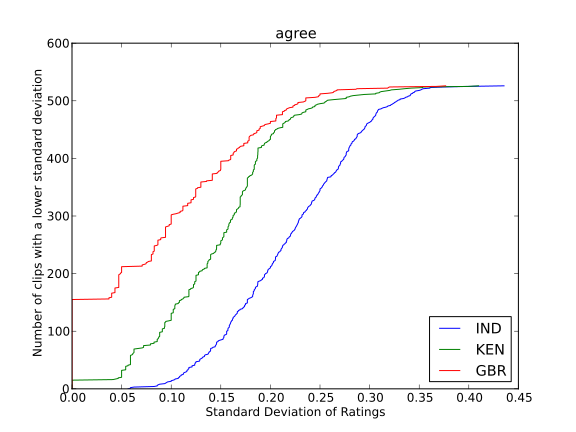
\includegraphics[width = 0.45 \columnwidth]{annotation/annotagree.pdf}
\includegraphics[width = 0.45 \columnwidth]{annotation/annotthinking.pdf}
\caption[Cumulative plot of the number of clips at various annotation standard deviations of annotator ratings.]{Cumulative plot of the number of clips at various annotation standard deviations of annotator ratings. Left plot shows \textit{agree} and the right plot shows \textit{thinking}.}
\label{FigureAgreementOfAnnotators1}
\end{figure}

\begin{figure}
\centering
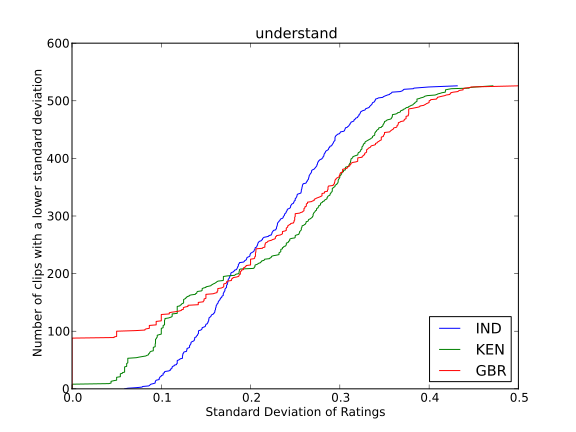
\includegraphics[width = 0.45 \columnwidth]{annotation/annotunderstand.pdf}
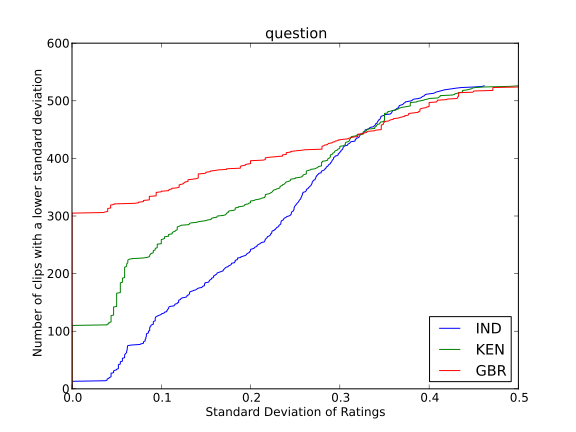
\includegraphics[width = 0.45 \columnwidth]{annotation/annotquestion.pdf}
\caption[Cumulative plot of the number of clips at various annotation standard deviations of annotator ratings.]{Cumulative plot of the number of clips at various annotation standard deviations of annotator ratings. Left plot shows \textit{understand} and the right plot shows \textit{question}.}
\label{FigureAgreementOfAnnotators2}
\end{figure}

\section{Conclusion}

\thesiscomment{DISCUSS If we have much more data, we could use unsupervised clustering without needing demographics. Or demographics can assist in semi-supervised clustering.}

This chapter has described the collection of cross cultural \ac{NVC} perception data. The data was collected based on paid Internet workers from multiple cultures. Because some workers did not cooperate with the task, the data was filtered to isolate the valid annotation data. The annotations were analysed and found to contain differences that were not merely linear scaling effects. This video annotation resulted in a new, cross cultural annotation of \ac{NVC} on natural informal conversations. The annotation data has been publicly released for further use. This helps to address the lack of publicly available \ac{NVC} annotation data. 

Crowdsourcing annotation data may prove to be a significant resource in human behaviour understanding if the quality issues can be addressed. The quality assurance tools that are currently available focus on annotation of discrete, objective labels. These objective labels are appropriate for computer vision tasks such as object recognition where the concepts are well defined. 
%An example question for object recognition can be as simple as a binary choice, e.g. ``Is there are car in this photograph?''. 
%Any disagreement in annotators usually indicates that the minority view is incorrect, based on the assumption that untrusted workers provide random responses rather than trying to sabotage the annotation exercise. 
However, discrete label filtering method is not useful in subjective tasks, such as \ac{NVC} annotation. In this case, inter-annotator disagreements do not necessarily imply that some of the annotators are wrong. Quality is still a significant concern and the filtering method proposed in this chapter is a step towards addressing this. The filtering method does rely on using the annotation mode, which depends on sufficient annotator participation to form a stable result. Also, the annotators are hard assigned to trusted and untrusted groups. It may be more efficient to use soft assignments for annotator trust.

The presence of cultural perception differences is not particularly surprising given a similar effect is often observed in emotion. The significance of the findings in this chapter is the confirmation of \ac{NVC} annotation differences and a quantitative analysis of the differences. The results suggest that different cultures have varying degrees of similarity. These perceptual cultural similarities might be exploited to reduce the number of \culturallySpecific perception models needed for \ac{NVC} recognition, possibly by treating actual annotator group perceptions as a mixture of two or more exemplar perception models.

There are significant shortcomings of Internet crowdsourcing for studying perception. The annotators are not screened and the environment in which the annotation is performed is not controlled. Each culture has a different availability of computer resources, different levels of computer literacy, different demographics that will undertake the task and the annotation is performed in different settings. These differences are known to be a factor in emotion perception and are likely to play a role in \ac{NVC} perception. The use of demographic questions may allow some of these variables to be controlled. This chapter has used English language questionnaires, but there can be cultural differences in the understanding of language. Given that perception differences in this chapter may be caused by either language perception differences or \ac{NVC} perception differences, it is hard to distinguish these effects. One possible method to check and possibly quantify language differences in crowdsource annotation is to conduct cross cultural annotation of data that has objective labels, using a single language questionnaire. If the annotators were consistent across cultures, this result would validate the approach of using a single language. Translation of \ac{NVC} survey instruments replaces the uncertainty of language perception with uncertainty over the validity of the translation of \ac{NVC} concepts, which by definition do not directly correspond to word based concepts.

%Emotion is studied by examining the response to an emotionally inducing stimuli. However, \ac{NVC} focuses on conscious action, rather than automatic reaction. It is possible that culturally equivalent stimuli do not exist for \ac{NVC}.

The next chapter uses this \continuous annotation data to approach the \ac{NVC} recognition problem by cross cultural regression.

\begin{savequote}
Behaviour is the mirror in which everyone shows their image.
\qauthor{Johann Wolfgang von Goethe}
\end{savequote}


\chapter[Multiple Culture NVC Regression]{Multiple Culture NVC Regression}
\label{ChapterNvcRegression}

\thesiscomment{MAIN POINT: Cultural differences make training and testing on different cultures problematic, and we solve this by having culture specific automatic systems to improve performance.}

\thesiscomment{WHAT we do}

\thesiscomment{HOW we do it}

\thesiscomment{RESULTS, IMPACT and NOVELTY}

The previous chapter has described the collection of \ac{NVC} signal annotations from three cultures: Great Britain (GBR), Kenya (KEN) and India (IND). This chapter will now apply this data to automatic \ac{NVC} regression. The three cultures present in the annotation data are treated as three separate ground truth sets. The annotation data is not combined into a global label set because this results in a label set that does not reflect the annotator perceptions (see Table \ref{MeanAnnotatorCorrelationTable}). This is because \culturallySpecific annotation data better reflects the annotator perception of \ac{NVC} used to create the data set (see Section \ref{SectionAnalysisOfCultureAnnotation}). Also, discrete groups of annotators enables us to train an \ac{NVC} recognition system with one culture's annotation set and test it using a different culture. This will experimentally show the performance of using training data that is dissimilar to the test culture. Most emotion and \ac{NVC} studies do not consider cultural differences but it is expected that the training and test data needs to culturally correspond to achieve good performance. This raises a potential problem, if current methods are deployed in different cultures without appropriately accounting for cultural difference. 
%This chapter demonstrates a possible solution to this issue: to train classifiers on a specific culture to better model that culture's specific properties. This will result in better performance in a wider range of potential applications.

The work builds upon the \ac{NVC} classifier described in Chapter \ref{ChapterClassification}, but changes are introduced to address some of the previous chapter's shortcomings. In summary, these improvements are:

\begin{itemize}
 \item use of \continuous labels, which makes this task a regression problem,
 \item use all the samples in the corpus, including intermediate intensity \ac{NVC} and examples of disagreement, rather than just the clear samples,
 \item use of a slightly different machine learning technique: $\nu$-SVR (pronounced nu-SVR),
 \item use of annotation data from three distinct cultures,
 \item the performance is evaluated by Pearson's correlation,
 \item only a single feature set is used (\textit{geometric-a}), 
 \item clips of various lengths are summarised into a fixed length ``digest'' vector by taking the feature mean and variance and
 \item only person independent testing is performed.
\end{itemize}

%These changes, their justifications and their implications will now be discussed.

In Chapter \ref{ChapterClassification}, the problem was simplified to two classes by considering only clear examples of each \ac{NVC} signal. This greatly reduces the amount of available training data. Every sample in the corpus is used in this chapter, with \continuous labels (see Section \ref{SectionSelectionOfNvcCategories}). This increases the difficulty of the task because intermediate strength \ac{NVC}s can be difficult to distinguish. This has previously been discussed, with respect to gaze and \textit{thinking}, in Section \ref{SectionVisualisingGaze}.

Because \ac{NVC} recognition is now expressed as a regression problem, different machine learning techniques must be used. Adaboost and standard \ac{SVM}s are binary classifiers and cannot be directly applied. Other techniques may be applied to regression, such as $\nu$-SVR \cite{Scholkopf2000} and this is described in the next section.

Three \culturallySpecific annotation sets are used, spanning four \ac{NVC} signals (\textit{agree}, \textit{thinking}, \textit{question} and \textit{understand}).
%Following from the definition of $\filteredAnnotation$ in the previous chapter, each video clip has a label matrix $\filteredAnnotation_{\cultureSelect} \in \mathbb{R}^{3 \times 4}$. 
%This significantly differs from most other supervised learning problems in that they are usually considered as a single value or class label. 
%This label matrix may be regressed by considering each component separately and training a regressor on each. For a label matrix of size $3$ by $4$, 
For the 3 cultures and 4 \ac{NVC} categories, $3\cdot4=12$ separate regression models are constructed and evaluated independently. It would be desirable achieve a good overall performance because an effective method should generalise to many different types of \ac{NVC} and operate in different cultures.

Feature tracking and feature extraction are used to transform digital frames into a form usable for effective machine learning. The method used is based on computing a statistical features based on the mean and variance of individual feature components. This encodes general activity level and facial expression without encoding the order of events. A statistical feature is a feature that is based on the statistical properties of a set of unordered observations. Statistical features are also known as temporal features \cite{Chantler1997, Meng2007, Mognon2010}, as well as ensemble features.
Only a single \featureGeneration approach is used in this chapter (\textit{geometric-a}), to limit the number of experiments to a manageable scale. This technique was selected because it had the highest overall performance and generalised well to unseen subjects in Chapter \ref{ChapterClassification}. 
%Polynomial \temporalFeatSingle were not used because they only provide a marginal improvement in classification performance (see Section \ref{SectionTemporalFeatures}). 
%Instead of using frame and clip level comparisons to measure a system's performance, a frame features from each clip are combined to form a clip digest vector of fixed length.

The approach involves \ac{NVC} regression of each label component based on a distinct, culture and \ac{NVC} specific models. There may be a wide range of possible interpretations for perceiving and interpreting \ac{NVC} (see Section \ref{BackgroundWhatFactorsInfluenceNvc}) because interpretation is dependent on context. 
%It is important to remember there is no ``wrong way'' to perceive \ac{NVC}. 
Given the number of potential factors that can affect perception, the number of specialised models may become too large to create or use in a practical application.
%To achieve a realistic model of human \ac{NVC} perception, it may be necessary to have person specific \ac{NVC} perception models. Given the vast resources required to construct billions of models, it is reasonable to ask if this approach is reasonable. A similar issue might be raise for automatic emotion recognition, if everyone expresses happiness in a slightly different fashion depending on many possible influences. 
However, the problem is not as insurmountable as it may at first appear. 
\begin{itemize}
 \item For a specific application of automatic \ac{NVC} recognition, there are probably a limited range of social and cultural situations which will be of interest.
 \item There are culturally and socially based similarities between humans, which greatly reduces the scale of the task.
 \item General models can be used as a basis and adapted to users during a brief, person specific training session. A similar approach is used in automatic speech recognition, in which a general model is adapted to a user's unique style of speaking.
\end{itemize}

Although it would be a vast undertaking to comprehensively solve the problem in every situation, \ac{NVC} recognition based on specific groups of annotators and in a specific application is feasible.

The main contributions of this chapter are:
\begin{itemize}
\item A study of recognition based on culturally distinct sets of annotators to better model \culturallySpecific \ac{NVC} perception. The automatic system uses \continuous \ac{NVC} labels which provide richer information content than discrete labels.
\item An analysis of the effect of training with one culture's annotations and testing on a different culture's annotation data.
\end{itemize}

The next section discusses the existing studies relevant to this work. Section \ref{SectionRegressionSystemOverview} provides an overview of the automatic system. Section \ref{SectionDigestVector} discusses how \temporalFeatSingle{ }are extracted and how regression is applied. Results are presented and discussed in Section \ref{SectionRegressionResultsAndDiscussion}.

\section{Related Research}
\label{BackgroundSupervisedRegression}

This section reviews the literature relating to facial analysis regression, temporal encoding by feature extraction and the use of multiple annotator groups. While there are many papers that use classification of emotion, there are relatively few that use regression. Many regression methods have been proposed but this section will focus on methods that have been applied to facial analysis. The most popular regression method is \ac{SVR} \cite{Drucker1997} that extended the \ac{SVM} algorithm, which was originally formulated as a binary classifier \cite{Vapnik1998}. 
%Using regression enables the use of continuous variable labels which provide a richer encoding of human behaviour. 
Emotion recognition has occasionally used \continuous labels such as valence, activation and dominance. Grimm \etal \cite{Grimm2007} used \ac{SVR} to predict these labels based on audio input. Kanluan \etal \cite{Kanluan2008} also used these labels for multimodal emotion recognition, with the modes combined by decision level fusion. They found that some label components were better recognized by audio and others by visual information. Some methods focus on modelling temporal variations while making \continuous predictions. Nicolaou \etal \cite{Nicolaou2011} used the related output associative \ac{RVM} technique for regression of valance-activation labels. W\"{o}llmer \etal \cite{Wollmer2008} found that neural networks can exceed the performance of \ac{SVR} for emotion regression. Both papers conclude that temporal modelling of features is important. Rudovic \etal \cite{Rudovic2012cvpr} used a prototypical emotion model to predict labels for different intensity emotions from the BU-4DFE dataset.

The previous paragraph has outlined papers that address emotion. There are few papers that use non-emotion labels based on facial analysis. Lucey \etal \cite{Lucey2009} used pain as a \continuous label of internal state. Savran \etal \cite{Savran2012} used regression for \ac{FACS} \ac{AU} regression using a hybrid {2D}/{3D} approach. Rudovic \etal used a  Laplacian-regularised Kernel Conditional Ordinal Random Field model for \ac{AU} intensity regression \cite{Rudovic2012}. Yang \etal \cite{Yang2009c} and Kim and Pavlovic \cite{Kim2010} approached the same problem using the concept of ranking of ordinal labels. Facial expression, pain, and emotion are often expressed without any conscious intention to communicate. Regression has not previously been applied to \ac{NVC} meaning.

As many authors have stressed, temporal encoding or modelling of human behaviour is critical to good recognition performance. One approach is to encode temporal variations by \featureGeneration. A simple way to achieve this is to calculate statistics of features in a temporal window. 
%Although many consider the fusion unordered temporal observations to not constitute ``temporal fusion'', this usage is consistent with the definition of temporal fusion given in Varshney\footnote{``Fusion of observations acquired at different times is referred to as temporal fusion.'' \cite{Varshney1997}} and Ko et al \cite{Ko2008}. 
Datcu and Rothkrantz \cite{Datcu2007} calculated variance of feature components in a sliding window and compared this to classification of individual frames, finding temporal encoding improves performance. Valstar \etal \cite{Valstar2006} used many forms of statistical measures, including symmetry. They found that measures that encoded maximal speed and displacement of the face, as well as order of co-occurrence were most useful in distinguishing posed from spontaneous brow movements. Petridis and Pantic used standard deviation and quadratic curve fitting of each of the feature components \cite{Petridis2008} in a temporal window. Grimm \etal \cite{Grimm2007} and W\"{o}llmer \etal \cite{Wollmer2008} computed statistical measures on audio features. Fang compares video sequences by using the mean of feature components \cite{Fang2009}. All these papers found that temporal encoding by \featureGeneration was an effective approach. However, the best encoding method may be task dependent. If many statistical measures are computed, the feature vector can become excessively large and this may require feature selection to isolate the important components.

%Perception modelling \cite{Massaro90}, \cite{Massaro96}

Several corpuses have used multiple annotators, as discussed in Section \ref{BackgroundMultipleAnnotation}. Typically, the annotation data is combined to form a single set of consensus labels. Hardly any studies consider groups of annotators as distinct and separate, and use this property in a machine learning context. Perhaps the only previous example of this is Reidsma's thesis \cite{Reidsma2008Thesis} which uses a subset of self-consistent annotators to train an automatic system that better reflects the perceptions of the annotator subset. However, this subset is not known to correspond to any particular meaningful group. Reidsma and op den Akker \cite{Reidsma2008b} considered each annotator separately and trained an independent model for each. Based on a test sample, each model votes to produce a final prediction by decision fusion. However, this approach is not used in this study because of the difficulty in motivating annotators to rate a significant proportion of the corpus which is required to train effective regression models. No existing work uses subjective labels from subsets of annotators that correspond to culturally or socially identifiable groupings, and then applies this as a basis for machine learning.

%The next section provides an overview of an automatic system that is trained on culturally distinct sets of annotators and uses regression of \ac{NVC} to provide continuous value predictions.

\section{Overview}
\label{SectionRegressionSystemOverview}

\begin{figure}
\centering
\includegraphics[width = 0.80 \columnwidth]{nvcregression/SystemOverview.pdf}
\caption{Overview of automatic system, showing filtering of annotations followed by training and testing on separate cultures.}
\label{SystemOverviewFigure}
\end{figure}

This section provides an overview of the automatic recognition system. The main steps are depicted in Figure \ref{SystemOverviewFigure}. \ac{LP} tracking is again used (see Section \ref{SectionLpTracking}). The tracking of each frame is then used to create a frame feature $\frameFeature_{alg}$ using the \textit{geometric-a} method (see Section \ref{SectionGenerateAlgorithmic}). The features are normalised on a per-subject basis, as defined in Equations \ref{EqnFeatureComponentMean} to \ref{EqnNormaliseFeatureRange}. For each annotated clip, these frame features are combined into a clip digest vector $\clipFeatureDigest$ using simple statistical measures. Each clip has a single digest vector and a matrix of labels $\filteredAnnotation$ (as described in Chapter \ref{ChapterAnnotation}). Eight fold cross validation is performed by dividing clips into person independent training and test sets. For each training fold, a $\nu$-SVR model is trained for each of the 12 components of $\filteredAnnotation$. The $\nu$-SVR models are then used to predict labels for the unseen samples in the test set. These predicted labels are compared to ground truth and the performance is evaluated by Pearson's correlation (in a similar fashion to \cite{Grimm2007, Kanluan2008}).

The details for feature extraction used to form the clip digest vector will be discussed in the next section, as well as some of the properties of $\nu$-SVR.

\section{\temporalFeatSingleCap{ }Extraction and Regression}
\label{SectionDigestVector}

This section describes the details of the regression system and the differences from the classification approach discussed in Chapter \ref{ChapterClassification}. Tracking and \featureGeneration is used to transform video frames into a form that can be used by standard machine learning techniques. As before, feature point tracking and \featureGeneration are performed by \acl{LP} trackers and \textit{geometric-a} features, previously introduced in Chapter \ref{ChapterClassification}. However these features consider individual frames separately and do not consider how the features vary over time. The clip digest vector, described below, encodes the feature variation over time.

%This section also outlines $\nu$-SVR as a regression technique. Regression is used because, unlike Chapter \ref{ChapterClassification}, the labels are considered as continuous variables.

%Feature generation encodes information about face deformation shape. We do not consider appearance based features, because they did not preform as well as shape features in classification. The LP flock tracking, previously discussed in Section \ref{SectionLpTracking}, is used. This provides position of facial features for the multi-culture annotated video clips (Section \ref{SectionMultiCultitureAnnotation}). We use either heuristic features (Section \ref{SectionGenerateHeuristic}) or algorithmic features (Section \ref{SectionGenerateAlgorithmic}) to create a feature vector which encodes information from a single frame.

\subsection{Computing the Clip Digest Vector by Feature Extraction}
\label{SectionClipFeatureExtraction}

Video clips in the corpus have variable lengths but an automatic system requires a way to compare the similarity of clips. Clip level and frame level performance measurement was introduced in Section \ref{SectionClassificationPerformance}. However, this approach was not particularly satisfactory because the frames were considered in isolation to produce a prediction by decision fusion. It would be preferable to consider how features vary across multiple frames. For this reason, the clip digest $\clipFeatureDigest$ is computed by taking the mean and variance of each feature component. The clip feature matrix $\clipFeature \in \mathbb{R}^{\numClipFrames \times \numFeatures}$, is summarised into a digest vector $\clipFeatureDigest \in \mathbb{R}^{2 \cdot \numFeatures}$. This fixed length vector $\clipFeatureDigest$ may then be used as an input to many standard machine learning tools, including $\nu$-SVR. For feature component $i$, 

\begin{gather}
 \clipFeatureDigest^{\clipId}_i = \overline{\clipFeature^{\clipId}_i}, i \in \{1...\numFeatures\} \\
 \clipFeatureDigest^{\clipId}_{i+\numFeatures} = \varFunc(\clipFeature^{\clipId}_{i+\numFeatures}), i \in \{1...\numFeatures\}
\end{gather}

where $\varFunc(\textbf{x})$ is the statistical variance of vector $\textbf{x}$. This is analogous to temporal quadratic features in Section \ref{SectionTemporalFeatures}, but instead of fitting a quadratic curve to a feature component, a Gaussian distribution is fitted to the frame samples. This decision was also based on the motion of eyes during thinking and the visualisation of feature space in Section \ref{SectionVisualisingGaze}. The main finding of that work was that there is little consistency in eye movement except for overall spread and offset from the origin, which can easily be encoded by taking the mean and variance of features. Neither this digest vector, nor the previous approaches of clip or frame level comparisons consider the order of the frames. However, it would be incorrect to say that these features are not temporal, because they do encode feature variation in multiple consecutive frames. Methods that consider the order of the frames have already been discussed elsewhere (e.g. polynomial features and Akak{\i}n and Sankur's work on \ac{HMM}s and \ac{CRF}s in Section \ref{SectionHmm}). Based on these findings, the claim that the frame order is a panacea for all \ac{NVC} and emotion recognition problems cannot be justified.

\thesiscomment{DISCUSS normalisation of features based on Equation \ref{EqnNormaliseFeatureRange}. This is applied to both feature sets?}

\thesiscomment{DISCUSS the drawbacks that mean and variance are not robust statistics}

\thesiscomment{DISCUSS is this approach only appropriate for clips of limited length?}

\subsection{Support Vector Regression and Performance Evaluation}
\label{SectionRegressionAndPerformanceEvaluation}

$\nu$-SVR \cite{Scholkopf2000} is used to perform regression of \ac{NVC} signals. 
%This technique is related to \ac{SVM}s previously used in Section \ref{SectionSupportVectorMachines}. 
$\nu$-SVR is similar to \ac{SVM}s in that it uses weighted kernels centred on sample points to specify a non-linear transform from feature space to a space that is more suitable. In the case of $\nu$-SVR, the distance from the feature space hyperplane is used to perform the regression, rather than just to separate the space into two regions as done by \ac{SVM}s. As in the case of classification, an \ac{RBF} kernel is used.

\thesiscomment{DISCUSS why RBF and the NU variant?}

%See also classification section \ref{SectionClassificationPerformance}

Because the labels are \continuous variables, the method used to assess performance must be considered. \ac{ROC} analysis, as used in previous chapters, only applies to two class problems. A performance metric that operates on \continuous variables is required. Pearson's correlation coefficient is used, as previously introduced in Section \ref{SectionAnalysisOfMeanRatings}. %This performance metric is sensitive to outliers but insensitive to scale differences between two compared variables. This is advantageous if robustness of the system is critical for an intended application but this measure may be over sensitive if this is not a priority. 
Person independent testing is conducted, rather than multi-person testing, because the person independent case has a broader range of applications than multi-person testing and because it is more challenging. 

\section{Results and Discussion}
\label{SectionRegressionResultsAndDiscussion}

This section discusses the experimental results of the automatic \ac{NVC} regression system. 
%The system was tested using eight fold, person independent cross validation. 
The parameters for $\nu$-SVR of $C = 1.0$ and $\nu = 0.5$ where found to be effective.

\thesisstatement{The NVC be regressed at above chance levels and the performance is comparable to humans(?)}

\begin{figure}
\centering
\includegraphics[width = 0.60 \columnwidth]{nvcregression/ScatterThinkUk.pdf}
\caption{Scatter plot of ground truth and automatically predicted \textit{thinking} \ac{NVC} intensities for the \ac{UK} culture. Each point corresponds to a single video clip.}
\label{ThinkScatterFigure}
\end{figure}

The predicted labels and ground truth labels are plotted in Figure \ref{ThinkScatterFigure} for a single \ac{NVC} category (\textit{thinking}) and for a single culture \textit{GBR}. A perfect system would have a linear arrangement of sample points. As can be seen, the distribution of points is certainly not linear, but an overall trend can be observed. 
%The density of points in the bottom left and top right are greater than the top left and bottom right quadrants. 
The Pearson correlation of this distribution is $0.46$ (a score of 1 being perfect correlation and 0 indicating no correlation). There are more samples on the left than on the right area of the plot. This is related to the annotated frequency of different intensity \ac{NVC} signals (see Figure \ref{RatingScoresFigure}). %There is a significant minority of samples that are outliers from the ideal distribution, which is likely to be penalised by Pearson's correlation. However 
The majority of points fall close to where a linear regression line would fall, which implies that most samples have a relatively good \ac{NVC} prediction.

\begin{table}
\centering
\caption[Correlation of automatic system for training and testing on a single culture.]{Correlation of automatic system for training and testing on a single culture. The error limits are one standard deviation of the individual cross validation correlation results. Figure \ref{ThinkScatterFigure} shows the individual ratings for \ac{UK} thinking \ac{NVC}. Note that this table uses a different performance metric than in Chapter \ref{ChapterClassification}, therefore the performance values cannot be directly compared.}
\begin{tabular}{|c| c c c c | c |}
\hline
%Culture & Agree & Thinking & Understand & Question \\
Culture & Agree & Question & Thinking & Understand & Average\\
\hline
\hline
India & 0.38$\pm$0.11 & 0.20$\pm$0.14 & 0.33$\pm$0.13 & 0.23$\pm$0.13 & 0.29\\
Kenya & 0.43$\pm$0.15 & 0.15$\pm$0.19 & 0.39$\pm$0.20 & 0.43$\pm$0.17 & 0.35\\
GBR & 0.27$\pm$0.08 & 0.16$\pm$0.21 & 0.46$\pm$0.20 & 0.37$\pm$0.13 & 0.32\\
\hline
Average & 0.36 & 0.17 & 0.39 & 0.34 & \\
%Global & 0.45$\pm$0.15 & 0.45$\pm$0.19 & 0.50$\pm$0.17 & 0.19$\pm$0.17 \\
\hline
\end{tabular}
\label{CultureCorrelationTable}
\end{table}

\thesisstatement{Different cultures have different NVC regression performances}

Figure \ref{ThinkScatterFigure} shows only one of the \ac{NVC} signals and in a single culture. With annotation data from multiple cultures on four \ac{NVC} categories, the performance of different \ac{NVC} signal regression models can be compared. As can be seen in Table \ref{CultureCorrelationTable}, the performance of some \ac{NVC} signals is low, particularly \textit{question} \ac{NVC}. The difficulty of \textit{question} recognition was previously seen for classification in Section \ref{SectionNvcClassificationResults}. Similarly, \textit{thinking} has the best performance in both regression and classification (see Table \ref{TableAlgorithmicFeatures}). This is unsurprising because both approaches use similar \featureGeneration and machine learning techniques. 
%This may be be caused by \ac{NVC} signals, such as \textit{question}, which rely on a verbal component which is not used in this system. 
Intense expressions of \textit{question} \ac{NVC} are relatively rare in this corpus and the regression algorithm may have difficulty learning a general model if insufficient positive samples are provided. In contrast, \textit{thinking} is relatively common and has a distinct visual appearance, making it easier for a visual system to recognise (see Section \ref{SectionVisualisingGaze}).

Each culture has a different average performance. This may be because one or both of:

\begin{itemize}
 \item the culture's annotators use facial features that are encoded with varying degrees of success by \textit{geometric-a} features.
 \item the quality of annotation varies across culture. IND culture had the largest proportion of untrusted annotators (see Section \ref{SectionAnnotationFilterMethod}) which might indicate a quality problem. It is also possible that different cultures may contain different levels of diversity in \ac{NVC} perception which may affect the validity of the consensus labels $\filteredAnnotation$.
\end{itemize}

%The performance may also be related to the quality of the annotation data.
The annotation labels are based on a mean consensus score $\filteredAnnotation$ for each question (described in Section \ref{SectionAnnotationFilterMethod}). However, individual annotators often differ from these consensus ratings. The human annotator correlation with the culture consensus is shown in Figure \ref{MeanAnnotatorCorrelationTable}. It is questionable if exceeding these performances would be meaningful, because the labels would not correspond to any specific, observable human perception of \ac{NVC}. The human correlation therefore provides an upper ceiling on the performance of our automatic system. This could be addressed by having a focused subset of annotators that have a higher inter-annotator agreement.

The performance of \ac{NVC} signal recognition is at an intermediate level and certainly far from being a reliable prediction. This is due to the extremely challenging nature of the task. The confounding factors include:

\begin{itemize}
 \item most \ac{NVC} signals are quite subtle and can be masked by larger face deformation cause by emotion and head pose changes,
 \item human behaviour in spontaneous conversations is much more variable than posed behaviour (Section \ref{BackgroundWhyIsNvcDifficult}), so the feature space to label partitioning is likely to be complex,
 \item spontaneous behaviour is hard to track, which increases input noise and
 \item some \ac{NVC} signals are based on verbal information which is not considered in this system.
\end{itemize}

\thesiscomment{DISCUSS variance error bars of scores?}

A system with a performance such as this may be useful for some applications where robustness is not a critical requirement. For example, in video retrieval, a list of candidates for clear examples of \ac{NVC} for a human to make a final section could use a noisy regression system to rank the examples. A wider range of applications could be addressed if better performance can be attained. 
%The issue of performance improvement of automatic systems is discussed again in the next chapter. This section returns to examining performance results, and other conclusions can be drawn from the experiments.

\begin{table}
\centering
\caption{Correlation of performance of the automatic system when training and testing on the same or different cultures.}
\begin{tabular}{ | c | c  c  c | }
\hline
Test & \multicolumn{3}{c|}{Train Culture} \\
Culture & India & Kenya & GBR \\
\hline
\hline
India & \cellcolor[gray]{0.9}0.29 & 0.27 & 0.24\\
Kenya & 0.27 & \cellcolor[gray]{0.9}0.35 & 0.33 \\
GBR & 0.25 & 0.33 & \cellcolor[gray]{0.9}0.32 \\
\hline
\end{tabular}
\label{CrossCulturePerformanceTable}
\end{table}

\thesisstatement{Cultural differences are significant in automatic NVC regression (training on the wrong culture results in worse performance)}

Table \ref{CrossCulturePerformanceTable} considers the case of training the automatic system on annotations from a single culture (either GBR, KEN or IND) and testing on annotations from a second culture (again either GBR, KEN or IND). The table diagonal, marked with a grey background, contain the performance of the system in the case where the training culture matches the test culture. For these tests, the results from different \ac{NVC} categories were combined by taking the average performance of the four \ac{NVC} signal performances. The most important point of this table is the diagonal performance values broadly exceed the performance values that are off diagonal. This shows that training a system in one culture's \ac{NVC} annotation and then testing on a different culture results in a performance loss. 
%This has implications for applications of automatic \ac{NVC} recognition. 
Current practice is to consider automatic \ac{NVC} and emotion recognition systems in a single culture and a single social situation. These results suggest this will not be an optimal approach if the culture specific model is intended to be used in a wider range of cultures. Although this result might be expected based on cross cultural research, this is the first quantitative measurement of the effect. This table also suggests a possible solution to the problem: to train specialised systems on appropriate cultural perception data to achieve better performance. The implementation of a cross culture \ac{NVC} recognition system is one of the primary contributions of this thesis.

\begin{figure}
\centering
\includegraphics[width = 0.15 \columnwidth]{nvcregression/clip_3dcfiL5Per_col_small.jpg}
\includegraphics[width = 0.65 \columnwidth]{nvcregression/clip_3dcfiL5Per.pdf}
\caption{Example frames, annotator ratings and predicted scores for corpus clip ``3dcfiL5Per'', in the GBR culture.}
\label{ExampleClipRatings1}
\end{figure}

\begin{figure}
\centering
\includegraphics[width = 0.15 \columnwidth]{nvcregression/clip_GyUrjdl6VT_col_small.jpg}
\includegraphics[width = 0.6 \columnwidth]{nvcregression/clip_GyUrjdl6VT.pdf}
\caption{Example frames, annotator ratings and predicted scores for corpus clip ``GyUrjdl6VT'', in the GBR culture}
\label{ExampleClipRatings2}
\end{figure}

To illustrate typical predictions that are made by the automatic system, two random video samples will be examined in more depth. The random video clips are shown in Figures \ref{ExampleClipRatings1} and \ref{ExampleClipRatings2}. The first ``3dcfiL5Per'' clip prediction shows that the predicted (blue) bars are in close agreement with the annotation ratings (red) in three of the \ac{NVC} categories (\textit{agree}, \textit{thinking} and \textit{understand}). However, the annotators have identified this clip as asking a question, resulting in a high score for \textit{question}. The automatic system, has in this case, failed to provide an appropriate prediction.

The second clip ``GyUrjdl6VT'' (Figure \ref{ExampleClipRatings2}) shows that all four predictions are at least approximately correct. The NVC categories \textit{agree} and \textit{question} are almost exactly correct, while the labels for \textit{thinking} and \textit{understand} are in rough agreement. These two figures imply the system is broadly making useful predictions but occasionally has significant errors. 
%This might indicate that some instances of \ac{NVC} are easier to identify than others.

\begin{figure}
\centering
\includegraphics[width = 0.85 \columnwidth]{nvcregression/PlotMeanOrVarianceOnlyFig.pdf}
\caption[The performance of the automatic system using either feature mean statistics or feature variance statistics or the original approach of using both mean and variance statistics.]{The performance of the automatic system using either feature mean statistics or feature variance statistics or the original approach of using both mean and variance statistics. The \ac{NVC} categories and cultures have been combined by taking the average performance.}
\label{FigureMeanOrVarianceCompared}
\end{figure}

As discussed in Section \ref{SectionClipFeatureExtraction}, \featureGeneration was performed by taking the clip mean and clip variance of each component of $\frameFeature_{alg}$. When either the mean features or variance features were disabled, the performance was reduced (see Figure \ref{FigureMeanOrVarianceCompared}). Using only mean based features resulted in a higher performance than just using the variance based features. The mean of features encodes facial expression shape, while variance of features encodes how much motion or activity there is in a local area of the face. This suggests that static face expression contains more information than facial activity for some \ac{NVC} signals. However, there may be more subtle temporal variations that contain relevant \ac{NVC} information. The best performance is when both of these approaches are combined and implies that facial expression and facial activity contain complementary information. Several papers have noted that temporal information is crucial in effective emotion recognition (see Section \ref{BackgroundSupervisedRegression}). Based on the results of this chapter, this holds true of \ac{NVC} as well as for emotion. Perhaps future work can find improved statistical measures that better encode the information to improve system performance.

\begin{figure}
\centering
\includegraphics[width = 0.85 \columnwidth]{nvcregression/MeanVarPlotWithCategories.png}
\caption[The performance of the automatic system using either feature mean statistics or feature variance statistics or the original approach of using both mean and variance statistics.]{The performance of the automatic system using either feature mean statistics or feature variance statistics or the original approach of using both mean and variance statistics. Each \ac{NVC} category is separately shown.}
\label{FigureMeanOrVarianceComparedWithCategories}
\end{figure}

The role of facial expression and facial activity can be investigated for individual \ac{NVC} categories. Each \ac{NVC} involves different gestures and different areas of the face. Figure \ref{FigureMeanOrVarianceComparedWithCategories} shows the performance of using only mean statistics or only variance statistics for each category. For most \ac{NVC} categories, both variance and mean statistics provide the best approach for automatic regression. However, the performance for \textit{understand} is approximately equal if the mean statistics approach is compared to the combined mean and variance approach performance. This implies that variance does not contain any complementary information for \textit{understand} \ac{NVC}. It is possible that some \ac{NVC} expressions may be recognized by purely static facial expressions. However, three \ac{NVC} signals require both facial expression and the temporal variation of expression for optimal performance.
%General conclusions are now drawn based on the findings of this chapter.

\section{Applying Digest Vector to \ac{NVC} Classification}
\label{SectionDigestVectorOnClassification}

The concept of encoding a video clip into a fixed length digest vector may also be applied to the person dependent classification problem discussed in Chapter \ref{ChapterClassification}. The approach described in the preceding section is slightly modified to make it suitable for binary class labels and \ac{AUC} performance evaluation. As in Chapter \ref{ChapterClassification}, only clear examples of \ac{NVC} are used, which is a less challenging problem than using all samples in the corpus.

Algorithmic features are generated on video frames and normalised as described in Section \ref{SectionGenerateAlgorithmic}. A digest vector is then computed for each video clip using the method described in Section \ref{SectionClipFeatureExtraction}. A $\nu$-SVC classifier \cite{Scholkopf2000} was trained using two fold cross validation of training and test data. As well as providing a conventional binary label prediction, $\nu$-SVC can provide a prediction of the class membership probability of an unseen sample. This was used in an \ac{ROC} analysis to determine the \ac{AUC} performance.

The performance is sensitive to the $\nu$-SVC cost parameter $C$. The parameter was determined for each fold of the training data independently. Parameter search of cost values of $\{10^{-2},$ $10^{-1},$ $10^{0},$ $10^{1},$ $10^{2}\}$ was performed on the training data on a leave one sample out basis. The cost parameter with the best \ac{AUC} performance was used to train a final classifier on the entire set of train data.

The performance of the system is shown in Table \ref{TableDigestMethodOnClassification}. The changes to \featureGeneration and classification result in a performance increase from 75\% to 85.4\%. This performance is an improvement on the previous state of the art, which was the overall performance of the \ac{HMM} approach proposed by Akak{\i}n and Sankur \cite{Akakin2011}. There are some \ac{NVC} signals, such as \textit{agree} and \textit{understand}, for which \ac{HMM} classification is still more effective than the method proposed here. The overall improvement in performance shows that for some \ac{NVC} signals, appropriate \featureGeneration can effectively encode temporal variations. In some cases, this can exceed the performance of some temporal classifier methods.

\begin{table}[tb]
\centering
\caption{\ac{AUC} performance, expressed as percentages. Testing is on a multi-person basis. The highlighted row corresponds to the method described in this chapter.}
\scriptsize 
\begin{tabular}{ c || c | c | c | c | c }
Method & Agree & Question & Thinking & Understand & Average \\
\hline
Akak{\i}n and Sankur, 2011 \cite{Akakin2011} & 85.9 & 78.2 & 83.8 & 83.6 & 82.9 \\
Sheerman-Chase \etal 2009 \cite{SheermanChase2009} & 70 & 73 & 81 & 80 & 76 \\
Result from Chapter \ref{ChapterClassification} & 70 & 70 & 83 & 75 & 75 \\
\hline
\cellcolor[gray]{0.8}Digest Vector, $\nu$-SVC & \cellcolor[gray]{0.8}81.4 & \cellcolor[gray]{0.8}89.7 & \cellcolor[gray]{0.8}95.8  & \cellcolor[gray]{0.8}74.8 & \cellcolor[gray]{0.8}85.4
\end{tabular}
\normalsize
\label{TableDigestMethodOnClassification}
\end{table}

\section{Regression on High Inter-annotator Agreement \ac{NVC} Signals}
\label{SectionRegressionHighAgreement}

The annotation consensus score $\filteredAnnotation^{\clipId}_{\nvcCategory}$ is formed by taking the mean of trusted annotator ratings. This assumes taking the mean of annotator ratings forms a meaningful \ac{NVC} label. However, the level of inter-annotator agreement, measured by rating variance, is different for each clip (see Section \ref{SectionInterAnnotatorAgreement}). By removal of clips of low inter-annotator agreement, it may be possible to remove data with meaningless labels from the corpus. However, if the filtering is too aggressive, useful and meaningful data may be discarded and the problem begins to become over-simplified.

Experiments were performed based on the method in Section \ref{SectionRegressionResultsAndDiscussion} except that only a subset of clips from the corpus was used for training and test. The subset was based on an inter-annotator threshold. Clips with a higher variance than the inter-annotator threshold were excluded. The system was tested with the inter-annotator threshold at various values. The correlation performance of these experiments are shown in Figures \ref{FigureInterannotatorFilteredPerformanceA} and \ref{FigureInterannotatorFilteredPerformanceB}.

\begin{figure}
\centering
\includegraphics[width = 0.49 \columnwidth]{nvcregression/interannotator/clipfilterperf-agree.pdf}
\includegraphics[width = 0.49 \columnwidth]{nvcregression/interannotator/clipfilterperf-thinking.pdf}
\caption[Correlation performance of automatic system after clips with a low inter-annotator agreement have been removed.]{Correlation performance of automatic system after clips with a low inter-annotator agreement have been removed. The left plot shows \textit{agree} and the right plot shows \textit{thinking}. Error bars of one standard deviation are shown.}
\label{FigureInterannotatorFilteredPerformanceA}
\end{figure}

\begin{figure}
\centering
\includegraphics[width = 0.49 \columnwidth]{nvcregression/interannotator/clipfilterperf-question.pdf}
\includegraphics[width = 0.49 \columnwidth]{nvcregression/interannotator/clipfilterperf-understand.pdf}
\caption[Correlation performance of automatic system after clips with a low inter-annotator agreement have been removed.]{Correlation performance of automatic system after clips with a low inter-annotator agreement have been removed. The left plot shows \textit{question} and the right plot shows \textit{understand}. Error bars of one standard deviation are shown.}
\label{FigureInterannotatorFilteredPerformanceB}
\end{figure}

As can be seen in these figures, reducing the threshold to focus on clips with higher inter-annotation agreement results in little overall change in performance. The greatest positive effect on performance is for \textit{thinking}, which may be due to the removal of ambiguous, multi-mode perceptions that may be present for this \ac{NVC} signal (see Section \ref{SectionInterAnnotatorAgreement}). The effect on \textit{agree} is detrimental, which suggests that the machine learning technique is robust to the label noise that is present, while inter-annotator agreement removes data that is useful for training. The other \ac{NVC} categories show no change or possibly a sight negative impact on performance.

Filtering the corpus based on inter-annotator agreement does not appear to be an effective way of improving performance in this case. It may be interesting to investigate the characteristics of \ac{NVC} samples that have higher and lower inter-annotator agreement, as well as the cause of agreement. The appropriateness of agreement metrics as the basis for machine learning could also be explored further \cite{Reidsma2008Thesis}. At present, we can say that the performance is relatively independent to the level of inter-annotator agreement filtering and this \ac{NVC} corpus contains some ambiguous label data which but this is not significantly detrimental to performance.

\section{Classification of Agreement and Disagreement in the Canal 9 Corpus}
\label{SectionCanal9}

The Canal 9 corpus comprises a series of Swiss/French TV studio political debates with a duration of 42 hours. The debates are between 2 to 4 participants and a moderator. The large number of subjects and the use of a single broadcasted view which has been edited from multiple cameras makes tracking more resource intensive. Having more than two participants and the TV cameras may result in increased head pose changes. The corpus has pre-existing annotation data which specifies the shot start/end and the identity of people in the shot. The quality is broadcast TV with interlaced frames. This annotation has been expanded to instances of agreement, disagreement and neutral by Bousmalis \etal \cite{Bousmalis2011} for a subset of shots that have a total duration of approximately 10 minutes and featuring 30 subjects. It is unclear if these annotations were intended to encode mental states or communicated meaning.

\begin{table}[tb]
\centering
\caption[Classification balanced accuracy performance for agreement and disagreement for the Canal 9 corpus.]{Classification balanced accuracy performance for agreement and disagreement for the Canal 9 corpus. The last two rows are the performance of the proposed method. Chance prediction performance is 50\% accuracy.}
\scriptsize 
\begin{tabular}{ c | c || c }
Classifier & Features & Balanced accuracy \\
\hline
SVM & hand/arm/shoulder gestures & 50\% \cite{Bousmalis2011}\\
SVM & prosody & 50\% \cite{Bousmalis2011}\\
SVM & hand/arm/shoulder gestures \& prosody & 52\% \cite{Bousmalis2011}\\
HMM & hand/arm/shoulder gestures & 43\% \cite{Bousmalis2011}\\
HMM & prosody & 51\% \cite{Bousmalis2011}\\
HMM & hand/arm/shoulder gestures \& prosody & 52\% \cite{Bousmalis2011}\\
HCRF & hand/arm/shoulder gestures & 51\% \cite{Bousmalis2011}\\
HCRF & prosody & 56\% \cite{Bousmalis2011}\\
HCRF & hand/arm/shoulder gestures \& prosody & 64\% \cite{Bousmalis2011}\\
\hline
NuSVC & facial \textit{geometric-h} & 50\% \\
NuSVC & facial \textit{geometric-a} & 51\% \\
\end{tabular}
\normalsize
\label{TableCanal9}
\end{table}

The problem is framed as a two class problem and evaluated in a five fold, ``leave one debate out'' cross validation by Bousmalis \etal \cite{Bousmalis2011}. They approached this problem by audio prosody feature extraction and manual hand/arm/shoulder gesture annotation, followed by training a temporal model classifier (\ac{HMM}s or \ac{HCRF}s) to provide automatic predictions. One static classifier was also used (\ac{SVM}). Their approach is similar to this thesis in that they do not use verbal information. Interestingly, they provide performance data for gestures, prosody and both combined. The performance metric used was balanced accuracy.

The method in this chapter is adapted to the Canal 9 data by using NuSVC\cite{Scholkopf2000} classification, which is closely related to the regression method used earlier. Faces were tracked using an extension of \ac{LP} tracking described in Sheerman-Chase \etal \cite{SheermanChase2013} and \textit{geometric-h}/\textit{geometric-a} geometric features are extracted (see Sections \ref{SectionGenerateHeuristic} and \ref{SectionGenerateAlgorithmic}). The features are normalised on a per-subject basis, as defined in Equations \ref{EqnFeatureComponentMean} to \ref{EqnNormaliseFeatureRange}. Multiple frames are combined by taking the feature component mean and variance as described in Section \ref{SectionClipFeatureExtraction}. NuSVR is used to provide a predicted class label.

The performance are shown in Table \ref{TableCanal9}. Just using the visual modality, including the method proposed in this chapter, results in chance level performance. Bousmalis \etal achieve the best results using prosody and arm gestures with \ac{HCRF}. This is likely to be the only result which is significantly above change, although this needs to be confirmed by more experiments. These results are surprising given the above chance classification and regression results using the TwoTalk corpus. There are a number of possible reasons for this result:

\begin{itemize}
 \item Visual features do not provide enough relevant information for humans or automatic methods to predict agreement and disagreement. (Although seeming not the case for TwoTalk)
 \item The facial area does contain relevant information, but the increase head pose changes and lower resolution of the face (typically 150 by 250 pixels in interlaced video) make tracking and extracting this information difficult.
 \item If relevant facial information is extracted, a non-dynamic model may not be suitable for classification. (Although it was suitable for TwoTalk.)
 \item The Canal 9 social context does not rely on facial behaviour for agreement and disagreement compared to the TwoTalk social context.
\end{itemize}

Judging by visual inspection, the tracking of the Canal 9 data seems to be relatively good. Either poor tracker of the different social context seems the most likely explanation for the poor performance. This raises the possibility that different social contexts require different approaches and even possibly different modalities to achieve effective behaviour or \ac{NVC} recognition. This may be an interesting area of future work.

%What about \cite{Bousmalis2012}?

\section{Classification of Mental States in the Mind Reading Corpus}
\label{SectionMindReading}

\begin{table}[tb]
\centering
\caption[Confusion matrix and classification accuracy of Mind Reading emotional states from el Kaliouby and Robinson \cite{ElKaliouby2004}, Figure 7.]{Confusion matrix and classification accuracy of Mind Reading emotional states from el Kaliouby and Robinson \cite{ElKaliouby2004}, Figure 7. Chance prediction performance is 17\%. Rows correspond to the true label, columns to predictions.}
\scriptsize 
\begin{tabular}{ c || c | c | c | c | c | c || c  }
\hline
mental state&agreeing&concentrating&disagreeing&interested&thinking&unsure&accuracy\\
\hline
agreeing	&\textbf{26}	&4	&0	&1	&0	&3	&76.5\%\\
concentrating	&1	&\textbf{16}	&0	&0	&0	&1	&88.9\%\\
disagreeing	&1	&1	&\textbf{17}	&0	&0	&2	&81.0\%\\
interested	&2	&2	&0	&\textbf{23}	&0	&3	&76.7\%\\
thinking	&1	&4	&0	&3	&\textbf{20}	&3	&64.5\%\\
unsure		&2	&3	&1	&0	&1	&\textbf{23}	&76.7\%\\
mean		&	&	&	&	&	&	&\textbf{77.4}\%\\
\end{tabular}
\normalsize
\label{TableMindReadingEK}
\end{table}

\begin{table}[tb]
\centering
\caption[Confusion matrix and classification accuracy of \textit{geometric-a} algorithmic features classified by NuSVC in one-against-all fashion.]{Confusion matrix and classification accuracy of \textit{geometric-a} algorithmic features classified by NuSVC in one-against-all fashion. Chance prediction performance is 17\%. Rows correspond to the true label, columns to predictions.}
\scriptsize 
\begin{tabular}{ c || c | c | c | c | c | c || c  }
\hline
mental state&agreeing&concentrating&disagreeing&interested&thinking&unsure&accuracy\\
\hline
agreeing	&\textbf{18}	&1	&6	&3	&6	&2	&50.0\%\\
concentrating	&2	&\textbf{2}	&1	&5	&3	&5	&11.1\%\\
disagreeing	&9	&0	&\textbf{3}	&1	&8	&3	&12.5\%\\
interested	&2	&2	&0	&\textbf{20}	&3	&3	&66.7\%\\
thinking	&6	&3	&4	&1	&\textbf{10}	&10	&27.8\%\\
unsure		&2	&1	&3	&3	&8	&\textbf{15}	&50.0\%\\
mean		&	&	&	&	&	&	&\textbf{36.3}\%\\
\end{tabular}
\normalsize
\label{TableMindReadingAlg}
\end{table}

\begin{table}[tb]
\centering
\caption[Confusion matrix and classification accuracy of \textit{geometric-h} heuristic features classified by NuSVC in one-against-all fashion.]{Confusion matrix and classification accuracy of \textit{geometric-h} heuristic features classified by NuSVC in one-against-all fashion. Chance prediction performance is 17\%. Rows correspond to the true label, columns to predictions.}
\scriptsize 
\begin{tabular}{ c || c | c | c | c | c | c || c  }
\hline
mental state&agreeing&concentrating&disagreeing&interested&thinking&unsure&accuracy\\
\hline
agreeing	&\textbf{19}	&1	&6	&3	&4	&3	&52.8\%\\
concentrating	&1	&\textbf{1}	&1	&4	&10	&1	&5.6\%\\
disagreeing	&7	&0	&\textbf{4}	&2	&8	&3	&16.7\%\\
interested	&4	&2	&1	&\textbf{19}	&0	&4	&63.3\%\\
thinking	&8	&5	&5	&1	&\textbf{8}	&9	&22.2\%\\
unsure		&2	&0	&2	&4	&12	&\textbf{10}	&32.3\%\\
mean		&	&	&	&	&	&	&\textbf{32.3}\%\\
\end{tabular}
\normalsize
\label{TableMindReadingHeur}
\end{table}

\begin{figure}
\centering
\includegraphics[width = 0.9 \columnwidth]{nvcregression/mindreadingperf.png}
\caption[Classification accuracy for Mind Reading mental states using various methods.]{Classification accuracy for Mind Reading mental states using various methods. Blue bars correspond to \textit{geometric-h} heuristic features classified by NuSVC in one-against-all fashion, orange bars correspond to \textit{geometric-a} algorithmic features classified by NuSVC in one-against-all fashion and yellow bars correspond to el Kaliouby and Robinson \cite{ElKaliouby2004}. Chance prediction performance is 17\%.}
\label{FigureMindReadingPerfSummary}
\end{figure}

Mind Reading Emotions Library is a commercial dataset that was originally developed for assisting those on the autism spectrum. The database comprises of 412 ``concepts'' or classes of mental states. Each concept has 6 silent videos of actors performing the mental state as well as 6 audio recordings. The database was published in 2004 and the video encoding is quite dated, with low quality compression and a small resolution of the face: typically 100 by 150 pixels. el Kaliouby and Robinson \cite{ElKaliouby2004} grouped some of these Mind Reading concepts into an arrangement of 6 classes (see Figure 3.2 in \cite{elKaliouby2005Thesis}). The mental states they studied were \textit{agreeing}, \textit{concentrating}, \textit{disagreeing}, \textit{interested}, \textit{thinking} and \textit{unsure}. This subset has 164 individual clips with a total duration of 19 minutes. These were used to train an automatic system based on a hybrid tracking and appearance features and a multi-scale temporal \ac{DBN} classifier. Ten sequences were discarded because the face tracker did not correctly initialise the head position for the first frame of the video clip. The particular clips excluded was not specified, making a replication of these experiments difficult. Performance evaluation was conducted on a ``leave one clip out'' basis and reported as classification accuracy. Their results are reproduced in Table \ref{TableMindReadingEK}. 

Although the labels in this corpus are superficially similar to the TwoTalk corpus used in this work, the labels of Mind Reading correspond to mental states and not to \ac{NVC} (see section \ref{BackgroundCompareContrastEmotionWithNvc}). However, it is possible to adapt the system proposed earlier in this chapter to the Mind Reading 6 class problem. As before,  features are tracked and \textit{geometric-h}/\textit{geometric-a} geometric features are extracted (see Sections \ref{SectionGenerateHeuristic} and \ref{SectionGenerateAlgorithmic}). The features are normalised on a per-subject basis, as defined in Equations \ref{EqnFeatureComponentMean} to \ref{EqnNormaliseFeatureRange}. Multiple frames are combined by taking the feature component mean and variance as described in Section \ref{SectionClipFeatureExtraction}. NuSVR in a one-vs-all arrangement is used to provide a predicted class label.

The confusion matrices of the proposed method are shown in Tables \ref{TableMindReadingAlg} and Table \ref{TableMindReadingHeur}. A class specific accuracy summary of these results and el Kaliouby and Robinson are shown in Figure \ref{FigureMindReadingPerfSummary}. As can be seen, the performance of the proposed method is significantly lower than that of el Kaliouby and Robinson. In particular, the mental state classes of \textit{concentrating} and \textit{disagreeing} are probably no better than chance predictions. \textit{thinking} is much better than chance, although further experiments are needed to establish the significance of most of these findings. \textit{unsure} and \textit{agreeing} are of intermediate performance but still far below el Kaliouby and Robinson's result. Only the \textit{interested} mental state is nearing el Kaliouby and Robinson's performance. As can be seen in the confusion matrices, \textit{unsure}, \textit{thinking} and \textit{concentrating} are often mistaken for one another. This is hardly surprising, since each of these mental states are very similar in outward behaviour and function. For the proposed method, the \textit{agreeing} accuracy exceeds the \textit{thinking} performance, while for \ac{NVC} the \textit{thinking} was recognized more consistently than \textit{agree} (see Figure \ref{CrossCulturePerformanceTable}). These effects many be cause by:

\begin{itemize}
 \item Acted behaviour is more intense and more consistent than spontaneous behaviour. This may be exploited by the temporal model used by el Kaliouby and Robinson to achieve a better result.
 \item \ac{NVC} and mental states are different concepts. The proposed system was developed for \ac{NVC} and el Kaliouby and Robinson's system was developed to address the Mind Reading corpus.
 \item There is less video data available for each class and more subjects in the Mind Reading corpus, which may affect which method is suitable. Specifically, the proposed method uses subject specific normalisation which can require a significant amount of data to reach a stable and robust model of facial behaviour.
 \item el Kaliouby and Robinson discarded video clips that were not tracked, while we consider all videos, which is a harder problem.
 \item The \featureGeneration technique used by each method is different, which may encode relevant information that is missed by other \featureGeneration approaches. Although the \textit{geometric-h} heuristic features are based on el Kaliouby and Robinson, it is not the same. They use appearance features that focus on mouth opening and teeth visible, which may be useful in distinguishing some of the classes.
\end{itemize}

The performance of the proposed system may be improved by feature selection or by the use of temporal model based classification. This is discussed in Section \ref{SectionMindReadingFeatureSelection}.

\section{Conclusion}

%As discussed in the previous chapter, there are cultural differences in \ac{NVC} perception. 
This chapter describes an automatic system that is trained on \culturallySpecific annotation data. This enables the automatic system to better model the cultural differences in \ac{NVC} perception. The predictions are \continuous labels, which provide richer information than using discrete \ac{NVC} class labels. All clips are used in this chapter, including examples of intermediate intensity \ac{NVC} and are tested in a person independent fashion. Simple geometric features are used, based on distances between pairs of trackers. Temporal information is encoded by taking simple statistical measures of feature components. %This results in an moderately effective \ac{NVC} regression system.

%\ac{NVC} is a subjective domain that is difficult to systematise without unintentionally over simplifying the problem. If a particular \ac{NVC} signal is expressed, it cannot be independently evaluated without human interpretation. 
Human interpretation can only be performed in a specific context. 
%It is difficult to separate cultural differences in expression from the effect of cultural perception with the limited data as used in this study. Also, 
It is difficult to determine if annotation differences are caused by perception differences, or cultural differences in the use of annotation tools. 
%\ac{NVC} signals do not precisely map on to word based concepts. This can make any attempt at translation questionable, if the \ac{NVC} concept being expressed is culturally specific. All these issues makes cross cultural study of \ac{NVC} challenging. 
There are a number of areas in which the current work could be improved. If natural conversations were recorded with \ac{NVC} encoders located in different cultures, effects of perceiving one's own culture vs. perceiving a different culture could be studied. Also, behaviour differences could be investigated, but it may be difficult to ensure each social situation is  equivalent across cultures to enable comparison. Better control of the annotators and encoders would also reduce the possibility that non-cultural effects being the dominant cause in differences of perception. Having the annotators work in a controlled environment and given the same instructions may perhaps improve consistency.

The general approach of specialised modelling of a culture's perception can be scaled to other cultures as long as training data is available. If every possible culture, social situation and personality requires a different model, the high resource requirements to produce these models makes this impractical. However, there are commonalities across social situations and cultures. Therefore, this commonality may be used to adapt an existing model to approximate a new culture or situation without retraining the system from scratch. This process may be similar to adaptation of a speech recognition system to a personalised accent.

Given the evidence that personality and gender affect emotion perception, it is possible these are factors in the perception of \ac{NVC}. Also, annotation data may be gathered without this information being available. It may still be possible to train a tailored system by unsupervised clustering of annotators based on their responses. This would make \ac{NVC} label predictions better reflect actual human responses but the personality type or gender of the annotators would be unknown. %This association between an annotator group and a specialised recognition system may be needed for some applications, but not in others.

The features used are based on an exhaustive extraction of distances between pairs of trackers. This can lead to the inclusion of irrelevant or redundant features, which can cause problems for machine learning algorithms. This can be addressed by feature selection and is discussed in the next chapter.

\begin{savequote}
Simplicity is the ultimate sophistication.
\qauthor{Leonardo da Vinci}
\end{savequote}

\chapter[Feature Selection for NVC Regression]{Feature Selection for NVC Regression}
\label{ChapterFeatureSelection}

\thesiscomment{WHAT we do}

\thesiscomment{HOW we do it}

\thesiscomment{RESULTS, IMPACT and NOVELTY}

%The previous chapter described an automatic system for \ac{NVC} regression. 
The features used in the two previous chapters were extracted based on distances between pairs of tracker positions. These features encoded local deformations of the face, with each feature component corresponding to a specific, local area. 
%The features were used to build a model of \ac{NVC} signals for recognition based on unseen samples. 
Expression of emotions or \ac{NVC} signals only involve part of the face but the features also encode areas of the face that are not involved in a specific \ac{NVC} expression. Therefore, the feature data contains irrelevant information. Redundant information is also present in the algorithmic features, with tracker motions in a local area of the face often being closely coupled. Training based on features that are largely irrelevant leads to over-fitting, in which the \ac{NVC} model is based on noise or incorrect features, rather than modelling the true underlying pattern. This results in poor generalisation and poor performance. This can be addressed by various means, including \featureGeneration that is focused on the task at hand, or by feature selection. 

Feature selection is the process of determining the relevance of features for a \ac{ML} task. Using a smaller subset of relevant features reduces the computational complexity of \ac{ML}. As the relevance of each feature is computed, this can give an insight to how \ac{NVC} is expressed. Feature selection provides a way to find associations between \ac{NVC} signals, relevant feature components and the associated areas of the face. Feature selection is a broad discipline with many approaches.
Features are either assigned a relevance weight or a subset of relevant features is found. This chapter uses an existing wrapper based approach which determines which subset of features is relevant. The selected feature subset can then be applied to \ac{NVC} recognition and the performance change can be evaluated.

An \ac{NVC} signal specific feature selection is computed for each culture. The performance contribution of each feature component is also evaluated. This results in a set of feature relevance weights for each \ac{NVC} signal. The feature weights can be visualised to show the involvement of facial areas in the expression of \ac{NVC} in an intuitive manner. This is based on segmenting a face using Voronoi tessellation around the position of trackers. Voronoi tessellation segments an image into cells based around seed positions; each point in the space is assigned to a cell based on the nearest seed position. This visualisation can either be used to check if the relevant facial areas conform to our expectation, or provide an indication as to the areas used by the automatic system. This in turn may provide clues as to human \ac{NVC} perception, although facial areas used in human perception of emotion may differ from an automatic approach.

The main contributions of this chapter are:

\begin{itemize}
 \item A method of feature selection to select subset of features that are relevant for \ac{NVC} recognition.
 \item A method of visualisation of the relevant features that is easy and intuitive to interpret.
\end{itemize}

The next section provides an overview of relevant existing research. Section \ref{SectionSbeFeatureSelection} discusses feature selection for the purposes of improving performance.

\section{Related Research}

There are many approaches to feature selection, which vary in performance, computational cost and restrictions on the type of input data. There are three general types of feature selection (see Saeys \etal for a review \cite{Saeys2007}):

\begin{itemize}
 \item filter methods, that consider feature components either individually or in groups, but do not consider the \ac{ML} method used to make the final prediction. This scales to large sets of features. These methods do not consider effect of the \ac{ML} method and may ignore the effects of combining groups of features.
 \item wrapper methods, that consider sets of features in conjunction with an \ac{ML} method. They do consider groups of features in context with \ac{ML} but they tend to be computationally intensive, they are classifier specific and are prone to over fitting.
 \item embedded methods, which are combined with \ac{ML} methods to select features. This makes the feature selection methodology and results specific to the \ac{ML} method used.
\end{itemize}

Existing papers that use feature selection for facial analysis will now be discussed. The use of an embedded feature selection, such as a boosting classifier, can be used to weight a set of features based on relevance. This feature subset can then be used by a second, more sophisticated classifier. This approach was used by Valstar \cite{Valstar2006} to select shape features by Gentleboost, and Petridis and Pantic \cite{Petridis2008} used Adaboost to select relevant audio and visual features. However, performing feature selection in this way, assumes there is similarity in the optimal set of features for both methods, which might not be the case. Yang \etal \cite{Yang2009} propose a feature selection method based on rough set theory on audio visual features. This avoids discretisation of feature values, as required by Adaboost, which may result in a loss of information. Filter based feature selection appears to have been largely avoided, probably because the number of feature components in the original feature vector is relatively low (usually thousands of feature components at most), and the interaction between features is often significant for emotion and \ac{NVC} recognition.

Wrapper based methods include randomised feature selection approaches such as simulated annealing and genetic approaches, but these have not been popular in facial analysis. Deterministic wrapper based approaches have been applied to emotion recognition: Grimm \cite{Grimm2007} used \ac{SFS} to isolate relevant audio features. This method begins with an empty set and incrementally adds features that produce the greatest performance increase, in a greedy fashion. An alternative, called \acf{SBE}, is to start with a full set of features and incrementally eliminate features that result in the best performance \cite{Kittler1978}. The \ac{SBE} approach was used by el Kaliouby and Robinson \cite{ElKaliouby2004} to find the most relevant geometric features.

There are several existing papers that identify which features have been selected for emotion or \ac{NVC} recognition, but it is less common to attempt to visualise which features have been selected. If features are shown, they are often visualised individually (e.g. \cite{Yang2009}), which can make comprehension of the overall distribution difficult. In experimental psychology, gaze patterns in perception have been visualised \cite{Jack2009}. Busso and Narayanan visualised areas of the face that were correlated with prosodic and vocal tract features for different emotions \cite{Busso2007}. It would be beneficial to have a method that is similar to these approaches for visualisation of feature selection results in a way that can be intuitively understood. 
%The next section will apply feature selection to the problem of \ac{NVC} recognition.

\section{\acs{SBE} Feature Selection}
\label{SectionSbeFeatureSelection}

%The previous chapter used geometric features to transform feature point tracking into a form that can be used by conventional \ac{ML} techniques. The geometric features (\textit{geometric-a}) are based on the distance between pairs of feature point trackers. However, this feature is likely to contain a great deal of redundant information. These features also contain noise from tracking drift and occasional occlusions. These noisy, redundant features result in a lower performance, as the regression model can have difficulty determining which features are relevant. This is addressed by using a technique to select the relevant features and remove those that are noisy or redundant. 
The approach used is a greedy \ac{SBE} of the features \cite{Kittler1978}. This section describes the method in detail and the resulting performance impact. 
%The advantage of \ac{SBE} is that interactions between subsets of variables are exploited. The main disadvantages of the method are possible over-fitting and a high computational cost.
Backward searching was thought to be preferable to forward searching because the interaction of features can be found and exploited. Forward search, particularly in the first few iterations, adds features without the benefit of other complimentary features. In contrast, a backward search allows irrelevant features to be eliminated while retaining features that contain complementary information. Also, it is possible to accelerate the backward search by removing more than one feature at each iteration, which reduces the computational cost.
Some feature component subsets are more effective than others. Unfortunately, \ac{SBE} may not find a globally optimal feature subset. If all possible feature subsets are considered as a space, \ac{SBE} performs a gradient descent to minimise error. 
%This type of search is not guaranteed to find a global optimum. 
% Alternative approaches, such as a forward-backwards search and exhaustive search were not used because they require higher computational resources and it is difficult to find approximations that reduce the computational cost to a practical level. The next section describes feature selection by \ac{SBE}.

\subsection{Method}

Feature selection occurs within a person independent, cross validation framework. There are eight folds in cross validation, resulting in eight different partitionings of seen and unseen data sets. Feature selection is applied to the seen data of a specific cross validation fold, to determine a relevant feature subset. \ac{SVR} is then applied to the feature subset to produce a model suitable for prediction.

%\begin{figure}[tb]
%\centering
%\includegraphics[width = 0.7 \columnwidth]{featureselection/feature-select.pdf}
%\caption{High level overview of feature selection. Features are selected by a greedy backward elimination, beginning with a %feature set that contains all possible features. The feature set at each stage is stored for later use. The detail of the ``select features for removal'' block is shown in Figure \ref{FigureFeaturesToRemove}.}
%\label{FigureFeatureSelectOverview}
%\end{figure}

\begin{algorithm}
\scriptsize 
\lstset{language=Python}
\begin{lstlisting}[frame=single]
def PerformFeatureSelection(data, labels):

   #The current mask begins with every feature enabled
   currentMask = np.ones((data.shape[1]), dtype=np.bool)

   #For storing the intermediate steps during feature selection
   allMasks = []

   #While more than one feature remains in the current mask
   while currentMask.sum() > 1:

      #Evaluate which features to remove
      toRemove = EvaluateRemainingFeatures(currentMask, data, labels)

      #Update the current mask and remove features
      for featToRemove in toRemove:
         currentMask[featToRemove[1]] = False

      #Store mask for later analysis
      allMasks.append(currentMask)

   return allMasks
\end{lstlisting}
\normalsize
\caption{Features are selected by a greedy backward elimination, beginning with a feature set that contains all possible features. The feature set at each stage is stored for later use. The algorithm is expressed as Python 2.7 code. The function \textit{EvaluateRemainingFeatures} is defined in Algorithm \ref{AlgFeaturesToRemove}.}
\label{AlgFeatureSelectOverview}
\end{algorithm}

The procedure for \acs{SBE} is shown in Algorithm \ref{AlgFeatureSelectOverview}. %Figure \ref{FigureFeatureSelectOverview}.
The search begins with a current set $\currentFeatureSet = \{1...\numFeatures\}$ which is initialised to include all possible feature components. The components to be removed from $\currentFeatureSet$ at each iteration is then determined. The current set $\currentFeatureSet$ is then updated and the process continues until the current set $\currentFeatureSet$ is empty. For the large number of components, it is too time consuming to remove components at a rate of 1 per iteration. To accelerate the process, multiple feature components are removed nearer the start of the \ac{SBE} process. As the number of components in the current set approaches zero, the rate of feature elimination returns to the standard 1 feature component per iteration. This produces a significant speed increase, but risks the removal of non-optimal components and this may result in a sub-optimal final feature set. The number of feature components removed from the current feature set at each iteration is denoted $\numToRemoveInMask$. This depends on the number of feature components $\numFeaturesInMask$ in the current set $\currentFeatureSet$ as follows:

\begin{gather}
\label{EquationNumFeaturesToRemove}
\numToRemoveInMask = \begin{cases}
200 : \numFeaturesInMask > 1000 \\
100 : \numFeaturesInMask > 400, \numFeaturesInMask \le 1000 \\
1 : \numFeaturesInMask \le 400
\end{cases}
\end{gather}

These thresholds were based on an intuitive expectation that only a small subset of features are required for accurate recognition.

%\begin{figure}[tb]
%\centering
%\includegraphics[width = 0.9 \columnwidth]{featureselection/select-features-to-remove.pdf}
%\caption{Each feature in the current feature set is tested. The features that cause the best performance are retained and the %features that worsen performance are preferred for removal. The detail for block marked ``test single feature'' is shown in Figure \ref{FigureTestSingleFeature}}
%\label{FigureFeaturesToRemove}
%\end{figure}

\begin{algorithm}
\scriptsize 
\lstset{language=Python}
\begin{lstlisting}[frame=single]
def EvaluateRemainingFeatures(mask, data, labels):

   #Determine how many components to remove, based on the mask
   numToRemove = CalcNumToRemove(mask.sum()) 

   #Initalise an empty list, based on the number of components in the mask
   scores = [None for count in range(mask.sum())] 

   #For each remaining component in the mask
   for count, featNum in enumerate(np.where(mask == True)[0]):

      #Create a test mask with a single component disabled
      testMask = np.copy(currentMask)
      testMask[featNum] = False

      #Evaluate the perfomance of the test mask and store the score
      scores[count] = (TestPerf(data[:, testMask], labels), featNum)

   #Return a list of features to remove
   scores.sort()
   scores.reverse()
   return scores[:numToRemove]
\end{lstlisting}
\normalsize
\caption{Each feature in the current feature set is tested. The features that cause the best performance are retained and the features that worsen performance are preferred for removal. The function \textit{TestPerf} is defined in Algorithm \ref{AlgTestSingleFeature}.}
\label{AlgFeaturesToRemove}
\end{algorithm}

To find an appropriate subset of features for removal from the current feature set, the contribution of each feature component needs to be assessed. An overview of this process is shown in Algorithm \ref{AlgFeaturesToRemove}. %Figure \ref{FigureFeaturesToRemove}. 
Each feature component in the current feature set $\currentFeatureSet$ is selected as the test component and the performance impact of the removal of the component is evaluated. The features are then prioritised, with the feature components resulting in the lowest performance preferred for removal. This process becomes progressively faster as the current feature set becomes smaller.

%\begin{figure}[tb]
%\centering
%\includegraphics[width = 0.7 \columnwidth]{featureselection/test-single-feature.pdf}
%\caption{The feature being tested is temporarily removed from the feature set. The system is then tested to check what effect this has on overall performance. This is carried out in another inner, ``feature selection'' cross validation loop.}
%\label{FigureTestSingleFeature}
%\end{figure}

\begin{algorithm}
\scriptsize 
\lstset{language=Python}
\begin{lstlisting}[frame=single]
def TestPerf(maskedData, labels):

   #Prepare cross validation sets
   kf = cross_validation.KFold(len(maskedData), numFolds)

   #Create an empty list for predictions
   allPredictions = [] 
   allLabels = []

   for train, test in kf: #For each cross validation fold

      #Fit a regression model on the training data
      regressor.fit(maskedData[train,:], labels[train])

      #Store the predictions based on the test data
      allPredictions.extend(regressor.predict(maskedData[test,:])) 

      #Store the test labels in this fold
      allLabels.extend(labels[test]) 

   #Calculate the overall correlation of predictions and test labels
   return np.corrcoef(allPredictions, allLabels)[0,1]
\end{lstlisting}
\normalsize
\caption{Testing the performance of a test set of feature components. The regression can use any suitable method, but in this study $\nu$-SVR is used.}
\label{AlgTestSingleFeature}
\end{algorithm}

To test a specific feature component, regression models are trained and tested to assess the performance of the remaining feature components as shown in Algorithm \ref{AlgTestSingleFeature}. %Figure \ref{FigureTestSingleFeature}. 
A temporary set $\tempFeatureSet$ is created which creates a copy of the current set $\currentFeatureSet$ except for the removal of the test component $i$:

\begin{gather}
\tempFeatureSet = \{j: j \in \currentFeatureSet, j \ne i\}
\end{gather}

The feature data is split into cross validation folds. These ``feature selection'' folds are distinct from the ``system'' cross validation folds discussed earlier, so that each fold contains data from multiple human subjects.

This produces a series of sets $\{\currentFeatureSet^\numFeatures..\currentFeatureSet^1\}$ that correspond to each stage in the progressive removal of features. Each set contains a different number of feature components. The performance of the feature set on the unseen data can then be determined. The expectation is for an increase in performance as poor features are removed. As the \ac{SBE} process is nearing termination, some features that are critical to \ac{NVC} regression are removed and the performance sharply declines. The performance of the feature subset at each stage is evaluated and retained for later analysis.

Because this process results in multiple sets which are used to create multiple \ac{NVC} models, it is not obvious which feature set to use and how many feature components are optimal. Simply selecting the peak performance when evaluating feature sets on unseen data violates the separation of seen and unseen data. For simplicity, this section uses the feature set $\currentFeatureSet^{unseen}$ having the peak performance for unseen test data to determine the number of feature components. It is likely that different \ac{NVC} signals require a specific set of geometric features to be effective. Therefore, feature selection is computed for a specific \ac{NVC} category and using a specific culture's annotation data. The processing of test set $\tempFeatureSet$ has been parallelized in this implementation, resulting in a speed increase. The next section uses the set $\currentFeatureSet^{seen}$ having the highest performance on seen training data only.

\subsection{Results}
\label{SectionFeatureSelectionUnseenPeak}

\begin{figure}[tb]
\centering
\includegraphics[width = 0.7 \columnwidth]{featureselection/shuffle-gbr-think/shufflefs-reverse-GBR-thinking-3008.pdf}
\caption[The performance of the system progressively improves as backward feature selection eliminates poor features.]{The performance of the system progressively improves as backward feature selection eliminates poor features. The upper line shows the seen data, which is used in the feature selection algorithm. The lower line shows the performance of the unseen data. The unseen data corresponds to subject 3008.}
\label{FigureShuffleGbrThink}
\end{figure}

%\ac{SBE} feature selection is performed by progressively removing features based on their effect on \ac{NVC} regression performance. 
A typical plot of performance against the number of feature components in the subset is shown in Figure \ref{FigureShuffleGbrThink}. As expected, the performance of predicting unseen test data increases as features are removed until performance suffers a sharp decline. The far left starting point of the lower curve corresponds to the performance of the system discussed in the previous chapter (i.e. without feature selection). In this example, feature selection results in a significant increase in performance. A feature set containing between 10 to 275 features encompasses the highest performance, with the peak performance requiring only 10 features. This feature set is smaller than the terse $\frameFeature_{geometric-h}$ features (Section \ref{SectionGenerateHeuristic}). However, it is unlikely that this feature set will be effective for other non-\textit{thinking} \ac{NVC} regression. This can be a disadvantage because the \ac{SBE} method is \ac{NVC} category specific and a great deal of computation is required to retrain the system for a different \ac{NVC} signal.

The feature selection curves are relatively linear until approximately 400 features remain. This corresponds to the threshold in Equation \ref{EquationNumFeaturesToRemove}. The change in the curve behaviour at this point suggests that a different set of thresholds might result in a higher peak, although this was not investigated.

\begin{figure}[tb]
\centering
\includegraphics[width = 0.49 \columnwidth]{featureselection/shuffle-gbr-think/shufflefs-reverse-GBR-question-1011.pdf}
\includegraphics[width = 0.49 \columnwidth]{featureselection/shuffle-gbr-think/shufflefs-reverse-KEN-agree-1011.pdf}
\caption[Additional examples of performance increases as feature selection progresses.]{Additional examples of performance increases as feature selection progresses. The left plot shows GBR \textit{question} performance. The right plot shows KEN \textit{agree} performance. Both unseen data folds correspond to subject 1011.}
\label{FigureShuffleFeatureSelect}
\end{figure}

This pattern is repeated for most other \ac{NVC} categories and in different cultures. While almost every test fold subject benefits from the feature selection process, not all system cross validation folds yield the same level of performance increase. The left plot of Figure \ref{FigureShuffleFeatureSelect} shows an instance in which feature selection was not effective. The performance is low before feature selection begins, which might indicate a problem with the approach in recognizing this subject performing \textit{question} \ac{NVC} signals. The right curve shows typical feature selection behaviour in a different culture (KEN in this case). A typical gradual improvement in performance can be seen, as features are removed before a sharp decline.

%Use of unseen data to determine FS termination, which is kind of cheating, shuffled sets
\begin{table}[htb]
\centering
\caption[System performance with termination of features selection based on the peak of unseen performance.]{System performance with termination of features selection based on the peak of unseen performance. This violates the separation of training and test data but this shows the performance with an ideal termination point.}
\begin{tabular}{ | c | c | c | }
\hline
Area & NVC      & Terminate \\
     & Category & By Unseen \\
     &          & Peak \\
\hline
GBR & Agree & 0.588 \\
GBR & Question & 0.453 \\
GBR & Thinking & 0.617 \\
GBR & Understand & 0.640 \\
\hline
IND & Agree & 0.627 \\
IND & Question & 0.534 \\
IND & Thinking & 0.638 \\
IND & Understand & 0.647 \\
\hline
KEN & Agree & 0.648 \\
KEN & Question & 0.453 \\
KEN & Thinking & 0.654 \\
KEN & Understand & 0.636 \\
\hline
All & Average & 0.586 \\
\hline
\end{tabular}
\label{TableShuffledFoldsTerminationOnUnseenCheat}
\end{table}

The optimal number of features is not known before feature selection begins. 
%The peaks for the unseen and seen performance curves in Figure \ref{FigureShuffleGbrThink} correspond to different numbers of features. 
The peak of unseen performance is 10 features, while the peak for seen performance is at approximately 125 features (see Figure \ref{FigureShuffleGbrThink}). A simple approach to determine the optimal number of features is to use the peak performance of unseen data. The performance for this method is shown in Table \ref{TableShuffledFoldsTerminationOnUnseenCheat}. However, this method violates the separation of training and unseen test data. Therefore, the results should not be directly compared to performance results in the previous chapter. The table shows the performance with the ideal termination of feature selection. This table implies that if terminated at an appropriate point, \ac{SBE} can result in a significant performance gain. 
%The next few sections consider approaches to automatically determine the number of features at termination using only seen data.

\subsection{Terminate \acs{SBE} Based on Seen Training Data}
\label{SectionFeatureSelectionSeenPeak}

\begin{table}[htb]
\centering
\caption[Comparison of various approaches of termination of the feature selection process, along with the performance without feature selection from the previous chapter.]{Comparison of various approaches of termination of the feature selection process, along with the performance without feature selection from the previous chapter. Termination using the unseen peak, as discussed in Section \ref{SectionFeatureSelectionUnseenPeak}, is the upper limit for performance based on \ac{SBE}. Termination based on peak seen performance (highlighted) is discussed in Section \ref{SectionFeatureSelectionSeenPeak}.}
\begin{tabular}{ | c | c | c | c | c | }
\hline
Area & NVC       & Terminate & \cellcolor[gray]{0.8}Terminate & Without  \\
     & Category  & By Unseen & \cellcolor[gray]{0.8}By Seen   & Feature \\
     &           & Peak      & \cellcolor[gray]{0.8}Peak      & Selection \\
\hline
GBR & Agree      & 0.588 & \cellcolor[gray]{0.8}0.523 & 0.340 \\
GBR & Question   & 0.453 & \cellcolor[gray]{0.8}0.385 & 0.188 \\
GBR & Thinking   & 0.617 & \cellcolor[gray]{0.8}0.556 & 0.440 \\
GBR & Understand & 0.640 & \cellcolor[gray]{0.8}0.605 & 0.389 \\
\hline
IND & Agree      & 0.637 & \cellcolor[gray]{0.8}0.600 & 0.400 \\
IND & Question   & 0.534 & \cellcolor[gray]{0.8}0.458 & 0.236 \\
IND & Thinking   & 0.638 & \cellcolor[gray]{0.8}0.588 & 0.363 \\
IND & Understand & 0.547 & \cellcolor[gray]{0.8}0.498 & 0.257 \\
\hline
KEN & Agree      & 0.648 & \cellcolor[gray]{0.8}0.604 & 0.462 \\
KEN & Question   & 0.453 & \cellcolor[gray]{0.8}0.358 & 0.162 \\
KEN & Thinking   & 0.654 & \cellcolor[gray]{0.8}0.600 & 0.363 \\
KEN & Understand & 0.636 & \cellcolor[gray]{0.8}0.595 & 0.431 \\
\hline
All & Average    & 0.586 & \cellcolor[gray]{0.8}0.531 & 0.336 \\
\hline
\end{tabular}
\label{TableShuffledFoldsTerminationOnSeenComparison}
\end{table}

The number of features for termination of the feature selection process should be determined based on seen training data. This restriction represents a system which is less reliant on manual tuning of parameters. The peak training data performance can be used to determine when to terminate the feature selection process. This is likely to select a non-optimal number of features, but this approach respects seen and unseen data separation. The results may be compared to the regression system in the previous chapter. The performance of this method is shown in the highlighted column of Table \ref{TableShuffledFoldsTerminationOnSeenComparison}. Feature selection produces a large increase in performance over the method described in the previous chapter. Therefore, feature selection is beneficial for \textit{geometric-a} features because it removes irrelevant features and results in a feature subset that is more suited for the specific \ac{NVC}. The next section changes the feature selection folds to be person independent, rather than multi-person.

\subsection{Terminate \acs{SBE} on Person-Independent Folds}
\label{SectionPersonIndependentFeatureSelection}

Feature selection in this chapter uses multiple folds to determine the performance as features are eliminated (Algorithm \ref{AlgTestSingleFeature}). Previously, each fold contained multi-person data in which every subject in the seen data was present in each feature selection fold. This does not affect the overall system testing, which remains person independent throughout. This change may be advantageous because feature elimination would be based on a system that had been trained and tested on different subjects and may improve the generalisation. However, as feature selection is run iteratively, the system may begin to over fit the training data.

\begin{table}[htb]
\centering
\caption[Performance of the system using person independent feature selection folds (highlighted, Section \ref{SectionPersonIndependentFeatureSelection}), compared to feature selection on multi person folds (Section \ref{SectionFeatureSelectionSeenPeak}).]{Performance of the system using person independent feature selection folds (highlighted, Section \ref{SectionPersonIndependentFeatureSelection}), compared to feature selection on multi person folds (Section \ref{SectionFeatureSelectionSeenPeak}). There is little overall difference in performance.}
\begin{tabular}{ | c | c | c | c | c | }
\hline
Area & NVC       & \cellcolor[gray]{0.8}Person      & Multi- \\
     & Category  & \cellcolor[gray]{0.8}Independent & Person \\
     & Category  & \cellcolor[gray]{0.8}Folds       & Folds \\
\hline
GBR & Agree      & \cellcolor[gray]{0.8}0.492 & 0.523\\
GBR & Question   & \cellcolor[gray]{0.8}0.341 & 0.385\\
GBR & Thinking   & \cellcolor[gray]{0.8}0.581 & 0.556\\
GBR & Understand & \cellcolor[gray]{0.8}0.599 & 0.605\\
\hline
IND & Agree      & \cellcolor[gray]{0.8}0.571 & 0.600\\
IND & Question   & \cellcolor[gray]{0.8}0.522 & 0.458\\
IND & Thinking   & \cellcolor[gray]{0.8}0.554 & 0.588\\
IND & Understand & \cellcolor[gray]{0.8}0.487 & 0.498\\
\hline
KEN & Agree      & \cellcolor[gray]{0.8}0.630 & 0.604\\
KEN & Question   & \cellcolor[gray]{0.8}0.393 & 0.358\\
KEN & Thinking   & \cellcolor[gray]{0.8}0.598 & 0.600\\
KEN & Understand & \cellcolor[gray]{0.8}0.591 & 0.595\\
\hline
All & Average    & \cellcolor[gray]{0.8}0.530 & 0.531\\
\hline
\end{tabular}
\label{TableFeatureSelectionPersonIndependent}
\end{table}

The performance of termination based on person independent folds is shown in Table \ref{TableFeatureSelectionPersonIndependent}. Although there are minor differences in performance for \ac{NVC} categories, the overall performance is relatively unchanged. Using either of these methods, feature selection finds a subset of features that are specialised in recognition of a specific \ac{NVC} signal. The next section provides a method for visualising the feature subset and an interpretation of the visualisations.

\section{Visualising Selected Feature Subsets}
\label{SectionVisualiseFeatureSelection}

%The previous section has described the use of \ac{SBE} to find a subset of geometric features that are specialised for a particular \ac{NVC} signal. 
Each feature component in the feature selection subset corresponds to a pair of trackers. This provides information about which facial regions are used by the regression model for \ac{NVC} recognition. It is useful to know which areas of the face are involved in \ac{NVC} expression: to assist understanding of human behaviour and to develop effective feature extraction methods. 
%The original annotation data does not directly give us this information. However, by visualising the feature selection results, the areas of the face are involved in \ac{NVC} expression recognition can be seen.
In order to visualise areas of the face relevant to \ac{NVC} expression, each feature component of the \textit{geometric-a} feature is assigned a weight based on the contribution that the feature component makes to the performance. As feature component $i$ is removed at \ac{SBE} iteration $j$, an increase $\weightSingleFeature_j$ in performance from $\systemPerformance_{j-1}$ to $\systemPerformance_{j}$ where $(\systemPerformance_{j} > \systemPerformance_{j-1})$ indicates the component was detrimental and is ignored ($\weightSingleFeature \in \mathbb{R}^{\numFeatures}, \systemPerformance \in \mathbb{R}^{\numFeatures}$). If a component is removed and the performance drops, this indicates the component was relevant. 

\begin{gather}
\label{EquationWeightTracker}
\weightSingleFeature_{j} = \begin{cases}
|\systemPerformance_{j} - \systemPerformance_{j-1}| : \systemPerformance_{j} - \systemPerformance_{j-1} > 0 \\
0 : \systemPerformance_{j} - \systemPerformance_{j-1} \le 0
\end{cases}
\end{gather}

The modulus of the performance drop $\weightSingleFeature$ is added to the weight of the two trackers $\trackerWeight^a_{j}$ and $\trackerWeight^b_{j}$ that correspond to the component $i$ ($\trackerWeight \in \mathbb{R}^{\numTrackers \times \numFeatures}$). 

\begin{gather}
\trackerWeight^a_{j-1} = \trackerWeight^a_{j} + \weightSingleFeature_{j} \\
\trackerWeight^b_{j-1} = \trackerWeight^b_{j} + \weightSingleFeature_{j} \\
\end{gather}

After the \ac{SBE} process is run to completion, the tracker weights are normalised to form normalised weight $\trackerWeightNorm$ which makes the tracker maximum weight equal to one ($\trackerWeightNorm \in \mathbb{R}^{\numTrackers}$).

\begin{gather}
\trackerWeightNorm^x = \frac{\trackerWeight^x_{j=0}}{max(\trackerWeight)}
\end{gather}

\begin{figure}[tb]
\centering
\includegraphics[width = 0.49 \columnwidth]{featureselection/TrackerPositions.pdf}
\caption[Manual division of tracker points into a flexible and rigid sets.]{Manual division of tracker points into a flexible and rigid sets. Flexible points are shown in green. Rigid points are shown in cyan. Humans have relatively little ability to move these rigid facial points relative to the skull.}
\label{FigureRigidTrackers}
\end{figure}

\begin{figure}[tb]
\centering
\begin{tabular}{ cc }
Agree & Question \\
\includegraphics[width = 0.49 \columnwidth]{featureselection/baragree.pdf} &
\includegraphics[width = 0.49 \columnwidth]{featureselection/barquestion.pdf} \\
\includegraphics[width = 0.49 \columnwidth]{featureselection/barthinking.pdf} & 
\includegraphics[width = 0.49 \columnwidth]{featureselection/barunderstand.pdf}\\
Thinking & Understand \\
\end{tabular}
\caption[Bar charts showing the normalised weights of tracking features for the four \ac{NVC} categories.]{Bar charts showing the normalised weights of tracking features for the four \ac{NVC} categories. Rigid and non-rigid trackers are shown as different colours, which indicate the relative importance of expression vs. head pose in recognition. The tracker ID numbers correspond to the numbering in Figure \ref{FigureRigidTrackers}. Results are from GBR culture, with person independent folds in feature selection. Visualisation areas have been averaged across test folds.}
\label{FigureFeatureWeightBarCharts}
\end{figure}

To investigate the relative importance of head pose when compared to the role expression, the trackers have been manually divided into rigid and non-rigid facial points. The manual division of trackers is shown in Figure \ref{FigureRigidTrackers}. However, it is possible to automatically separate points into rigid and flexible sets, as described by Del Bue \etal \cite{DelBue2005}. The normalised tracker weights for each of the four \ac{NVC} categories are shown in Figure \ref{FigureFeatureWeightBarCharts}. All \ac{NVC} categories have significant weights assigned to trackers on flexible parts of the face, which implies expression is significant for \ac{NVC} recognition. The weights assigned to rigid trackers are relatively low for \textit{question} \ac{NVC} and to some extent in \textit{thinking}. This suggests that these \ac{NVC} signals are largely conveyed by expression, with head pose having little importance. In contrast, the rigid tracker weights have higher weights in \textit{agree}, which suggests that head pose has a role in the automatic recognition process. This confirms our expectation that agreement is often expressed by the nodding of the head. The weightings also show that the trackers that have low weightings for all of the studied \ac{NVC} signals. The lowest weighted tracker overall was number 22, which corresponds to a part of the eyebrow. This may indicate a problem with this tracker or this area is redundant for recognizing these types of \ac{NVC} signals.

Although each tracker weight corresponds to a specific area of the face, it is difficult to form an overall impression of which areas of the face are involved, based on these bar charts. A better approach is to visualise the relevant areas in relation to an actual face. However, the visualisation process is complicated by the head pose. 
%If features for head pose where included in the visualisation, they would emphasis areas of the face which are rigid.
Head pose changes are not localised to an specific area of the face and should be removed. The head pose is generally encoded by the distance between two rigid points on the face. Facial deformations can either be encoded by distances which are either between rigid to flexible facial points or between flexible to flexible facial points.
%Position and weight information for rigid points was discarded. 
The remaining non-rigid points correspond to the flexible regions of the face and are responsible for facial deformations. The facial areas are based on a Voronoi tessellation of the face \cite{Dirichlet1850}, based on tracker positions on a manually selected frontal view of the face. The normalised weights of each tracked point are used to control the saturation of the local area in the image. Relevant areas are shown as normal saturation. Irrelevant areas are shown as desaturated, which makes the colour tend to pure white for low weights. This enables an intuitive way to visualise relevant areas for \ac{NVC} expression around the face.

\begin{figure}[tb]
\centering
\begin{tabular}{ cc }
Agree & Question \\
\includegraphics[width = 0.39 \columnwidth]{featureselection/visoutput-agree-crop-bng.png} &
\includegraphics[width = 0.39 \columnwidth]{featureselection/visoutput-question-crop-bng.png} \\
\includegraphics[width = 0.39 \columnwidth]{featureselection/visoutput-thinking-crop-bng.png} & 
\includegraphics[width = 0.39 \columnwidth]{featureselection/visoutput-understand-crop-bng.png}\\
Thinking & Understand \\
\end{tabular}
\caption[Visualising the areas of face used for \featureGeneration.]{Visualising the areas of face used for \featureGeneration. The face is segmented based on Voronoi tessellation. More saturated areas indicate the importance of an area, less saturated areas are not relevant for a particular \ac{NVC}. Results are from GBR culture, with person independent folds in feature selection. Visualisation areas have been averaged across test folds.}
\label{FigureFeatureSelectionVis}
\end{figure}

The results of the visualisation are shown in Figure \ref{FigureFeatureSelectionVis}. The clearest example of facial areas corresponding to our expectation is for \textit{thinking}. The eyes are prominently selected and gaze is already thought to play a role in this \ac{NVC}, as discussed in Section \ref{SectionVisualisingGaze}. The other features provide an indication into less well understood \ac{NVC}. The brow region seems important for \textit{question} \ac{NVC}. When intense examples of \textit{question} are viewed, there is generally consistent brow lowering (action unit 4) lasting for less than a second which occurs at or near the end of a question sentence (see Figure \ref{FigureBrowLoweringQuestion}). The feature selection seems to be using this behaviour as the basis for recognition. This connection between verbal questioning and brow lowering has not been previously reported in published research, although Ekman mentions unpublished experiments which found this association \cite{Ekman1979}. Brow raising and lowering has also been documented in sign language but in this context, the direction of raising or lowering has a distinct semantic meaning, depending on the type of question that is being asked \cite{Ekman1999}. For \textit{agree} and \textit{understand}, the areas selected are less specific but generally indicate that the eyes and mouth are involved and the brow area is not used. While the visualisation shows areas that are involved in \ac{NVC} recognition by \ac{ML}, it does not necessarily imply that humans use these areas for recognition, but shows that information is present in these areas. However, there is a strong possibility that humans also use this information during \ac{NVC} perception.

\begin{figure}[tb]
\includegraphics[width = 0.49 \columnwidth]{featureselection/question-clip_1HTGE8FuGw.jpg}
\includegraphics[width = 0.49 \columnwidth]{featureselection/question-clip_4bg18VX1W3.jpg} \\
\caption{Brow lowering (action unit 4), lasting for less than a second, often occurs at or near the end of a question sentence.}
\label{FigureBrowLoweringQuestion}
\end{figure}

This approach could be improved by additional trackers, would would improve the spatial resolution of the visualisation. %Determining the relative importance of head pose might also be useful, particularly for \textit{agree} which can involve head nodding. %Visualisation of feature selection can provide clues as to how human perception operates.

\section{Applying Feature Selection to the Mind Reading Corpus}
\label{SectionMindReadingFeatureSelection}

Classification of mental states in the Mind Reading corpus was previously discussed in Section \ref{SectionMindReading}. This section applies feature selection to the algorithmic geometric features in an attempt to improve classification performance. The motivation is the save as in the case of TwoTalk: the feature vector contains irrelevant or redundant information which can reduce the performance of recognition. The experimental arrangement used is the same as described in Section \ref{SectionMindReading}, except for only a subset of features are used, as determined by Algorithm \ref{AlgFeatureSelectOverview}. Because cross validation evaluation is performed on a leave-one-clip-out basis, it is not computationally feasible to perform a separate feature selection for each of the 174 folds. In this case, feature selection is conducted on a two fold basis on the entire corpus. As the feature selection removes features by \ac{SBE}, the performance based on two fold classification accuracy rises. The change in performance during the \ac{SBE} process is shown in Figure \ref{FigureMindReadingPerfFeatureSbe}. The resultant masks are then evaluated using the standard level-one-clip-out; the classification accuracy of this is shown in Figure \ref{FigureMindReadingSbeTestPerf}. As usual, the performance gradually increases as unnecessary or detrimental features are removed, before a sudden reduction in performance. Peak performance for the feature selection occurs for between 50 and 90 feature components. A set of 88 feature components is manually selected, based on it having the best classification accuracy. The number of features removed at each stage is as follows:

\begin{gather}
\label{EquationNumFeaturesToRemoveMindReading}
\numToRemoveInMask = \begin{cases}
4 : \numFeaturesInMask > 1000 \\
2 : \numFeaturesInMask > 500, \numFeaturesInMask \le 1000 \\
1 : \numFeaturesInMask \le 500
\end{cases}
\end{gather}

This removes features more slowly than in the previous section, which should help prevent useful features being eliminated. However, this results in the system being evaluated at more stages during the \ac{SBE} process.

\begin{figure}
\centering
\includegraphics[width = 0.8 \columnwidth]{featureselection/mindreading-fs.pdf}
\caption{Classification accuracy of two-fold cross validation on the Mind Reading corpus as features are eliminated by \ac{SBE}.}
\label{FigureMindReadingPerfFeatureSbe}
\end{figure}

\begin{figure}
\centering
\includegraphics[width = 0.8 \columnwidth]{featureselection/mindreading-test.pdf}
\caption{Classification accuracy of level-one-clip-out cross validation on the Mind Reading corpus as features are eliminated by \ac{SBE}, based on the previously selected feature sets.}
\label{FigureMindReadingSbeTestPerf}
\end{figure}

\begin{figure}
\centering
\includegraphics[width = 0.8 \columnwidth]{featureselection/MindReadingFeatureSelectPerf.png}
\caption[Performance of various classification methods based on the Mind Reading Corpus.]{Performance of various classification methods based on the Mind Reading Corpus. Orange corresponds to algorithmic geometric features without feature selection (method described in Section \ref{SectionMindReading}). Green corresponds to the algorithmic geometric feature selection method proposed in this section, with 88 components. Yellow corresponds to el Kaliouby and Robinson \cite{ElKaliouby2004}. Chance prediction performance is 17\%.}
\label{FigureMindReadingAlgFs}
\end{figure}

\begin{table}[tb]
\centering
\caption[Confusion matrix of mental state classification using geometric algorithmic features with feature selection on the Mind Reading corpus.]{Confusion matrix of mental state classification using geometric algorithmic features with feature selection on the Mind Reading corpus. Feature selection resulted in a set of 88 feature components which are more effective at classification.}
\scriptsize 
\begin{tabular}{ c || c | c | c | c | c | c || c  }
\hline
mental state&agreeing&concentrating&disagreeing&interested&thinking&unsure&accuracy\\
\hline
agreeing	&\textbf{20}	&0	&4	&2	&5	&5	&55.6\%\\
concentrating	&0	&\textbf{0}	&2	&7	&3	&6	&0.0\%\\
disagreeing	&7	&0	&\textbf{8}	&2	&3	&4	&33.3\%\\
interested	&2	&2	&0	&\textbf{20}	&2	&4	&66.7\%\\
thinking	&5	&3	&2	&2	&\textbf{21}	&3	&58.3\%\\
unsure		&1	&2	&2	&2	&5	&\textbf{18}	&60.0\%\\
mean		&	&	&	&	&	&	&\textbf{45.6}\%\\
\end{tabular}
\normalsize
\label{TableMindReadingAlgFs}
\end{table}

The use of feature selection results in a significant performance increase but is still not as effective as el Kaliouby and Robinson \cite{ElKaliouby2004}. Classification for \textit{concentrating} is worse than chance classification and is often mislabelled as \textit{interested} or \textit{unsure}, which are arguable closely related to \textit{concentrating}. There are less examples of \textit{concentrating} in the corpus, which may be a factor in poor recognition performance for this class. Other reasons for the lower performance include:

\begin{itemize}
 \item Acted behaviour is more intense and more consistent than spontaneous behaviour. This may be exploited by the temporal model used by el Kaliouby and Robinson to achieve a better result.
 \item \ac{NVC} and mental states are different concepts. The proposed system was developed for \ac{NVC} and el Kaliouby and Robinson's system was developed to address the Mind Reading corpus.
 \item There is less video data available for each class and more subjects in the Mind Reading corpus, which may affect which method is suitable. Specifically, the proposed method uses subject specific normalisation which can require a significant amount of data to reach a stable and robust model of facial behaviour.
 \item el Kaliouby and Robinson discarded video clips that were not tracked, while we consider all videos, which is a harder problem.
 \item The \featureGeneration technique used by each method is different, which may encode relevant information that is missed by other \featureGeneration approaches. Although the \textit{geometric-h} heuristic features are based on el Kaliouby and Robinson, it is not the same. They use appearance features that focus on mouth opening and teeth visible, which may be useful in distinguishing some of the classes.
 \item Feature selection on geometric algorithmic features was conducted based on the performance of all classes. However, it may be more effective to have a one-vs-one class basis for feature selection, to better isolate features that distinguish each class.
\end{itemize}

\section{Conclusion}

%As seen in the previous chapter, features generated based on tracker distances can encode facial deformation as a step in \ac{NVC} recognition. 
Geometric features used in the previous chapter contain a great deal of redundant and irrelevant components. This chapter describes an \ac{SBE} based method to find a subset of features that are relevant for a specific \ac{NVC} signal. This removes feature components that are not relevant for \ac{NVC} recognition and this results in a significant performance increase. The feature subset is then visualised to show the facial areas used by the automatic system. This provides evidence of which facial areas are involved in the expression of each \ac{NVC} signal. Knowing the areas of the face used for \ac{NVC} can suggest feature types that better encode these local areas, avoids computation of irrelevant or redundant features, as well as improving our understanding of human behaviour.

The areas of the face that are used by the system either correspond to the expected areas, or for \ac{NVC} signals that are less well understood, they give an indication as to the facial areas that are involved. The areas used for each \ac{NVC} are different, which implies that the feature selection has isolated feature components that are specific to each \ac{NVC}. Thinking is known to involve gaze aversion and this is clearly seen in that feature components that encode eye movement are retained by the feature selection process. Based on reviewing corpus videos, it was manually observed that a sentence ending with a question is often accompanied by a brief brow lowering and this is also consistent with the visualisation of questioning \ac{NVC}.

\ac{SBE} feature selection was based on multiple folds of the seen data. Using folds that were either person-independent or person-dependent did not make a significant performance difference. The termination of the \ac{SBE} process was based on the peak performance of the training data used in the optimisation. This does not select the optimal number of features but it still resulted in a significant performance increase. If a system can be manually tuned, a slightly better performance can be achieved but the number of features that is optimal depends on the specific \ac{NVC}.

The visualisation of the feature selection subsets used annotation data from a single culture. It may be possible to investigate whether other cultures use different areas of the face for \ac{NVC} perception, based on feature selection. Gaze patterns are culturally dependent for emotion recognition \cite{Jack2009}. However, humans may be using different areas of the face for recognition, compared to an automatic system. This may be due to the feature extraction process not being as comprehensive as human perception. The areas used by an automatic system may provide indirect clues as to the way human perception operates. This cross cultural visualisation is not attempted in this thesis, because this would require a larger video corpus, more comprehensive facial encoding and additional annotation data to provide a reliable result.

Head pose has a role in \ac{NVC} but the visualisation in this chapter is focused on local facial deformations. The features are only considered as simplistic temporal variations. The temporal encoding currently considers an entire clip, so cannot temporally localise relevant motion in \ac{NVC} expression. However, with more detailed temporal encoding, which might consider variation in a sliding window, a particular time and area of the face could be identified as important for \ac{NVC} automatic regression. The feature selection framework also might provide a framework to extend the existing automatic system to other feature types. Considering many different areas of the face (or holistic facial features) over multiple time scales and temporal offsets will result in a vast number of potential features. For this reason, techniques that are suitable for spotting patterns in large data sets, such as data mining, may be relevant to facial analysis. %Also techniques that separate relevant features from irrelevant ones, such as feature selection, will reduce the quantity of features to a practical level.

The feature selection method presented here is a simple but computationally intensive approach. The removal of many features during the early iterations was necessary to make the approach practical but the performance implications of this approximation are not well understood. Other feature selection methods may be investigated to reduce the computation requirements and improve performance.

%The final chapter draws broad conclusions for the overall thesis and discusses the work in context.

\include{conclusion/conclusion}

%\appendix

%\appendix
\begin{appendices}
\chapter{Additional Classification Results}
\label{ChapterAdditionalClassificationResults}
\newpage
%Extracts from Tables \ref{SvmWindowPersonindepTable} and \ref{SvmClipPersonindepTable} were used in Tables \ref{TableAlgorithmicFeatures} and \ref{TabelHeuristicFeatures}. 
%Tables \ref{BoostWindowMultipersonTable} and \ref{SvmWindowMultipersonTable} contain additional sliding window, multi-person results and are included for completeness.


\begin{table}[H]
\centering
\caption{Adaboost, Multi-person testing, classification of sliding window examples. Mean and standard deviation performance is shown.}
\resizebox{0.6 \columnwidth}{!}{
\begin{tabular}{ c | c | c | c | c }
\hline
Test & Agree & Question & Think & Understand\\
\hline
affine & 0.62$\pm$0.09 & 0.52$\pm$0.03 & 0.53$\pm$0.06 & 0.64$\pm$0.03\\
deform-cubica & 0.51$\pm$0.11 & 0.60$\pm$0.04 & 0.57$\pm$0.03 & 0.51$\pm$0.06\\
deform-fastica & 0.51$\pm$0.11 & 0.60$\pm$0.04 & 0.57$\pm$0.03 & 0.51$\pm$0.06\\
deform-pca & 0.59$\pm$0.07 & 0.65$\pm$0.05 & 0.70$\pm$0.06 & 0.65$\pm$0.05\\
geometric-h & 0.64$\pm$0.09 & 0.69$\pm$0.04 & 0.60$\pm$0.07 & 0.65$\pm$0.05\\
geometric-a & 0.65$\pm$0.03 & 0.62$\pm$0.07 & 0.67$\pm$0.03 & 0.71$\pm$0.01\\
lbp & 0.57$\pm$0.08 & 0.67$\pm$0.03 & 0.57$\pm$0.04 & 0.59$\pm$0.04\\
lm & 0.56$\pm$0.11 & 0.66$\pm$0.03 & 0.59$\pm$0.04 & 0.46$\pm$0.05\\
\hline
affine-t & 0.62$\pm$0.09 & 0.52$\pm$0.03 & 0.53$\pm$0.06 & 0.64$\pm$0.03\\
deform-cubica-t & 0.52$\pm$0.12 & 0.60$\pm$0.04 & 0.58$\pm$0.03 & 0.51$\pm$0.06\\
deform-fastica-t & 0.46$\pm$0.13 & 0.61$\pm$0.05 & 0.58$\pm$0.03 & 0.49$\pm$0.06\\
deform-pca-t & 0.59$\pm$0.07 & 0.65$\pm$0.05 & 0.70$\pm$0.06 & 0.65$\pm$0.05\\
geometric-h-t & 0.64$\pm$0.09 & 0.69$\pm$0.04 & 0.60$\pm$0.07 & 0.65$\pm$0.05\\
lm-t & 0.56$\pm$0.11 & 0.66$\pm$0.03 & 0.60$\pm$0.03 & 0.46$\pm$0.05\\
\hline
\end{tabular}
}
\label{BoostWindowMultipersonTable}
\end{table}

\begin{table}[H]
\centering
\caption{Adaboost, Multi-person testing, classification of video clips}
\resizebox{0.6 \columnwidth}{!}{
\begin{tabular}{ c | c | c | c | c }
\hline
Test & Agree & Question & Think & Understand\\
\hline
affine & 0.59$\pm$0.08 & 0.54$\pm$0.03 & 0.51$\pm$0.03 & 0.60$\pm$0.02\\
deform-cubica & 0.50$\pm$0.11 & 0.61$\pm$0.05 & 0.59$\pm$0.02 & 0.49$\pm$0.04\\
deform-fastica & 0.50$\pm$0.11 & 0.61$\pm$0.05 & 0.59$\pm$0.02 & 0.49$\pm$0.04\\
deform-pca & 0.61$\pm$0.05 & 0.68$\pm$0.03 & 0.70$\pm$0.07 & 0.72$\pm$0.05\\
geometric-h & 0.64$\pm$0.09 & 0.71$\pm$0.04 & 0.66$\pm$0.08 & 0.69$\pm$0.04\\
geometric-a & 0.70$\pm$0.03 & 0.68$\pm$0.11 & 0.75$\pm$0.01 & 0.75$\pm$0.01\\
lbp & 0.58$\pm$0.06 & 0.68$\pm$0.04 & 0.60$\pm$0.06 & 0.62$\pm$0.05\\
lm & 0.55$\pm$0.06 & 0.65$\pm$0.02 & 0.59$\pm$0.03 & 0.46$\pm$0.05\\
\hline
affine-t & 0.59$\pm$0.08 & 0.54$\pm$0.03 & 0.53$\pm$0.05 & 0.59$\pm$0.03\\
deform-cubica-t & 0.51$\pm$0.12 & 0.61$\pm$0.05 & 0.59$\pm$0.02 & 0.49$\pm$0.04\\
deform-fastica-t & 0.45$\pm$0.14 & 0.64$\pm$0.05 & 0.60$\pm$0.00 & 0.48$\pm$0.04\\
deform-pca-t & 0.61$\pm$0.05 & 0.68$\pm$0.03 & 0.70$\pm$0.07 & 0.72$\pm$0.05\\
geometric-h-t & 0.64$\pm$0.07 & 0.71$\pm$0.04 & 0.66$\pm$0.08 & 0.69$\pm$0.03\\
lm-t & 0.55$\pm$0.06 & 0.65$\pm$0.02 & 0.60$\pm$0.02 & 0.46$\pm$0.05\\
\hline
\end{tabular}
}
\label{BoostClipMultipersonTable}
\end{table}

\begin{table}[H]
\centering
\caption{\ac{SVM}, Multi-person testing, classification of sliding window examples}
\resizebox{0.6 \columnwidth}{!}{
\begin{tabular}{ c | c | c | c | c }
\hline
Test & Agree & Question & Think & Understand\\
\hline
affine & 0.47$\pm$0.03 & 0.52$\pm$0.02 & 0.48$\pm$0.04 & 0.51$\pm$0.01\\
deform-cubica & 0.50$\pm$0.00 & 0.50$\pm$0.00 & 0.50$\pm$0.00 & 0.50$\pm$0.00\\
deform-fastica & 0.50$\pm$0.00 & 0.50$\pm$0.00 & 0.50$\pm$0.00 & 0.50$\pm$0.00\\
deform-pca & 0.50$\pm$0.02 & 0.54$\pm$0.02 & 0.53$\pm$0.03 & 0.54$\pm$0.01\\
geometric-h & 0.58$\pm$0.04 & 0.57$\pm$0.02 & 0.61$\pm$0.01 & 0.63$\pm$0.02\\
geometric-a & 0.66$\pm$0.06 & 0.67$\pm$0.05 & 0.74$\pm$0.01 & 0.73$\pm$0.03\\
lbp & 0.57$\pm$0.04 & 0.58$\pm$0.04 & 0.55$\pm$0.02 & 0.58$\pm$0.07\\
lm & 0.50$\pm$0.03 & 0.58$\pm$0.03 & 0.56$\pm$0.04 & 0.50$\pm$0.01\\
\hline
affine-t & 0.47$\pm$0.04 & 0.52$\pm$0.03 & 0.48$\pm$0.04 & 0.52$\pm$0.01\\
deform-cubica-t & 0.50$\pm$0.00 & 0.50$\pm$0.00 & 0.50$\pm$0.00 & 0.50$\pm$0.00\\
deform-fastica-t & 0.50$\pm$0.00 & 0.50$\pm$0.00 & 0.50$\pm$0.00 & 0.50$\pm$0.00\\
deform-pca-t & 0.50$\pm$0.04 & 0.61$\pm$0.03 & 0.55$\pm$0.06 & 0.54$\pm$0.02\\
geometric-h-t & 0.60$\pm$0.04 & 0.57$\pm$0.03 & 0.63$\pm$0.02 & 0.64$\pm$0.02\\
lm-t & 0.51$\pm$0.04 & 0.60$\pm$0.02 & 0.59$\pm$0.04 & 0.50$\pm$0.03\\
\hline
\end{tabular}
}
\label{SvmWindowMultipersonTable}
\end{table}

\begin{table}[H]
\centering
\caption{\ac{SVM}, Multi person testing, classification of video clips}
\resizebox{0.6 \columnwidth}{!}{
\begin{tabular}{ c | c | c | c | c }
\hline
Test & Agree & Question & Think & Understand\\
\hline
affine & 0.49$\pm$0.05 & 0.56$\pm$0.03 & 0.49$\pm$0.07 & 0.54$\pm$0.05\\
deform-cubica & 0.51$\pm$0.01 & 0.50$\pm$0.00 & 0.50$\pm$0.00 & 0.50$\pm$0.00\\
deform-fastica & 0.51$\pm$0.01 & 0.50$\pm$0.00 & 0.50$\pm$0.00 & 0.50$\pm$0.00\\
deform-pca & 0.50$\pm$0.02 & 0.61$\pm$0.02 & 0.56$\pm$0.07 & 0.49$\pm$0.03\\
geometric-h & 0.71$\pm$0.05 & 0.69$\pm$0.04 & 0.73$\pm$0.03 & 0.77$\pm$0.03\\
geometric-a & 0.70$\pm$0.06 & 0.70$\pm$0.06 & 0.83$\pm$0.01 & 0.75$\pm$0.03\\
lbp & 0.57$\pm$0.05 & 0.60$\pm$0.03 & 0.54$\pm$0.03 & 0.59$\pm$0.09\\
lm & 0.50$\pm$0.08 & 0.58$\pm$0.07 & 0.57$\pm$0.04 & 0.45$\pm$0.03\\
\hline
affine-t & 0.49$\pm$0.06 & 0.55$\pm$0.01 & 0.47$\pm$0.07 & 0.55$\pm$0.05\\
deform-cubica-t & 0.51$\pm$0.01 & 0.50$\pm$0.00 & 0.50$\pm$0.00 & 0.50$\pm$0.00\\
deform-fastica-t & 0.51$\pm$0.01 & 0.50$\pm$0.00 & 0.50$\pm$0.00 & 0.50$\pm$0.00\\
deform-pca-t & 0.55$\pm$0.02 & 0.65$\pm$0.03 & 0.57$\pm$0.06 & 0.55$\pm$0.04\\
geometric-h-t & 0.71$\pm$0.04 & 0.67$\pm$0.04 & 0.73$\pm$0.05 & 0.76$\pm$0.04\\
lm-t & 0.53$\pm$0.09 & 0.67$\pm$0.07 & 0.60$\pm$0.06 & 0.47$\pm$0.04\\
\hline
\end{tabular}
}
\label{SvmClipMultipersonTable}
\end{table}

\begin{table}[H]
\centering
\caption{Adaboost, Person independent testing, classification of sliding window examples}
\resizebox{0.6 \columnwidth}{!}{
\begin{tabular}{ c | c | c | c | c }
\hline
Test & Agree & Question & Think & Understand\\
\hline
affine & 0.61$\pm$0.02 & 0.42$\pm$0.09 & 0.50$\pm$0.03 & 0.55$\pm$0.04\\
deform-cubica & 0.55$\pm$0.07 & 0.52$\pm$0.08 & 0.55$\pm$0.06 & 0.45$\pm$0.04\\
deform-fastica & 0.55$\pm$0.07 & 0.52$\pm$0.08 & 0.55$\pm$0.06 & 0.45$\pm$0.04\\
deform-pca & 0.61$\pm$0.06 & 0.47$\pm$0.04 & 0.64$\pm$0.03 & 0.57$\pm$0.02\\
geometric-h & 0.66$\pm$0.06 & 0.61$\pm$0.06 & 0.52$\pm$0.06 & 0.56$\pm$0.06\\
geometric-a & 0.66$\pm$0.02 & 0.52$\pm$0.04 & 0.65$\pm$0.02 & 0.68$\pm$0.05\\
lbp & 0.57$\pm$0.04 & 0.53$\pm$0.13 & 0.49$\pm$0.07 & 0.44$\pm$0.05\\
lm & 0.56$\pm$0.03 & 0.54$\pm$0.10 & 0.50$\pm$0.14 & 0.41$\pm$0.04\\
\hline
affine-t & 0.62$\pm$0.02 & 0.47$\pm$0.04 & 0.49$\pm$0.03 & 0.55$\pm$0.03\\
deform-cubica-t & 0.59$\pm$0.01 & 0.56$\pm$0.06 & 0.51$\pm$0.02 & 0.47$\pm$0.01\\
deform-fastica-t & 0.55$\pm$0.07 & 0.52$\pm$0.08 & 0.55$\pm$0.06 & 0.45$\pm$0.04\\
deform-pca-t & 0.61$\pm$0.06 & 0.47$\pm$0.04 & 0.64$\pm$0.03 & 0.57$\pm$0.02\\
geometric-h-t & 0.66$\pm$0.06 & 0.61$\pm$0.06 & 0.53$\pm$0.08 & 0.56$\pm$0.06\\
lm-t & 0.57$\pm$0.03 & 0.56$\pm$0.09 & 0.50$\pm$0.14 & 0.41$\pm$0.04\\
\hline
\end{tabular}
}
\label{BoostWindowPersonindepTable}
\end{table}

\begin{table}[H]
\centering
\caption{Adaboost, Person independent testing, classification of video clips}
\resizebox{0.6 \columnwidth}{!}{
\begin{tabular}{ c | c | c | c | c }
\hline
Test & Agree & Question & Think & Understand\\
\hline
affine & 0.62$\pm$0.05 & 0.39$\pm$0.07 & 0.50$\pm$0.03 & 0.53$\pm$0.09\\
deform-cubica & 0.52$\pm$0.05 & 0.56$\pm$0.11 & 0.55$\pm$0.07 & 0.42$\pm$0.04\\
deform-fastica & 0.52$\pm$0.05 & 0.56$\pm$0.11 & 0.55$\pm$0.07 & 0.42$\pm$0.04\\
deform-pca & 0.68$\pm$0.05 & 0.50$\pm$0.09 & 0.69$\pm$0.08 & 0.60$\pm$0.04\\
geometric-h & 0.65$\pm$0.07 & 0.64$\pm$0.07 & 0.55$\pm$0.09 & 0.57$\pm$0.08\\
geometric-a & 0.70$\pm$0.03 & 0.58$\pm$0.08 & 0.74$\pm$0.03 & 0.71$\pm$0.06\\
lbp & 0.57$\pm$0.07 & 0.49$\pm$0.16 & 0.48$\pm$0.09 & 0.39$\pm$0.08\\
lm & 0.56$\pm$0.02 & 0.51$\pm$0.10 & 0.48$\pm$0.15 & 0.46$\pm$0.04\\
\hline
affine-t & 0.65$\pm$0.04 & 0.39$\pm$0.07 & 0.49$\pm$0.02 & 0.58$\pm$0.05\\
deform-cubica-t & 0.56$\pm$0.01 & 0.62$\pm$0.07 & 0.52$\pm$0.04 & 0.45$\pm$0.03\\
deform-fastica-t & 0.53$\pm$0.05 & 0.56$\pm$0.11 & 0.55$\pm$0.07 & 0.43$\pm$0.05\\
deform-pca-t & 0.68$\pm$0.05 & 0.50$\pm$0.09 & 0.69$\pm$0.08 & 0.60$\pm$0.04\\
geometric-h-t & 0.65$\pm$0.07 & 0.64$\pm$0.07 & 0.55$\pm$0.10 & 0.56$\pm$0.09\\
lm-t & 0.56$\pm$0.02 & 0.54$\pm$0.07 & 0.46$\pm$0.13 & 0.44$\pm$0.04\\
\hline
\end{tabular}
}
\label{BoostClipPersonindepTable}
\end{table}

\begin{table}[H]
\centering
\caption{\ac{SVM}, Person independent testing, classification of sliding window examples.
%\ref{TableAlgorithmicFeatures} and \ref{TabelHeuristicFeatures}.
}
\resizebox{0.6 \columnwidth}{!}{
\begin{tabular}{ c | c | c | c | c }
\hline
Test & Agree & Question & Think & Understand\\
\hline
affine & 0.49$\pm$0.03 & 0.51$\pm$0.04 & 0.45$\pm$0.04 & 0.50$\pm$0.03\\
deform-cubica & 0.50$\pm$0.00 & 0.50$\pm$0.00 & 0.50$\pm$0.00 & 0.50$\pm$0.00\\
deform-fastica & 0.50$\pm$0.00 & 0.50$\pm$0.00 & 0.50$\pm$0.00 & 0.50$\pm$0.00\\
deform-pca & 0.50$\pm$0.00 & 0.50$\pm$0.00 & 0.50$\pm$0.00 & 0.50$\pm$0.00\\
\rowcolor[gray]{.95} geometric-h & 0.59$\pm$0.02 & 0.51$\pm$0.02 & 0.52$\pm$0.02 & 0.56$\pm$0.02\\
\rowcolor[gray]{.95} geometric-a & 0.66$\pm$0.03 & 0.54$\pm$0.01 & 0.70$\pm$0.03 & 0.70$\pm$0.02\\
lbp & 0.55$\pm$0.05 & 0.51$\pm$0.11 & 0.49$\pm$0.08 & 0.47$\pm$0.08\\
lm & 0.50$\pm$0.00 & 0.51$\pm$0.01 & 0.49$\pm$0.01 & 0.51$\pm$0.00\\
\hline
affine-t & 0.49$\pm$0.03 & 0.52$\pm$0.04 & 0.46$\pm$0.04 & 0.50$\pm$0.03\\
deform-cubica-t & 0.50$\pm$0.00 & 0.50$\pm$0.00 & 0.50$\pm$0.00 & 0.50$\pm$0.00\\
deform-fastica-t & 0.50$\pm$0.00 & 0.50$\pm$0.00 & 0.50$\pm$0.00 & 0.50$\pm$0.00\\
deform-pca-t & 0.50$\pm$0.00 & 0.51$\pm$0.01 & 0.50$\pm$0.00 & 0.50$\pm$0.00\\
\rowcolor[gray]{.95} geometric-h-t & 0.60$\pm$0.02 & 0.51$\pm$0.02 & 0.55$\pm$0.02 & 0.58$\pm$0.02\\
lm-t & 0.51$\pm$0.00 & 0.51$\pm$0.01 & 0.48$\pm$0.01 & 0.50$\pm$0.01\\
\hline
\end{tabular}
}
\label{SvmWindowPersonindepTable}
\end{table}

\begin{table}[H]
\centering
\caption{\ac{SVM}, Person independent testing, classification of video clips. %\ref{TableAlgorithmicFeatures} and \ref{TabelHeuristicFeatures}.
}
\resizebox{0.6 \columnwidth}{!}{
\begin{tabular}{ c | c | c | c | c }
\hline
Test & Agree & Question & Think & Understand\\
\hline
affine & 0.53$\pm$0.05 & 0.56$\pm$0.07 & 0.48$\pm$0.02 & 0.56$\pm$0.04\\
deform-cubica & 0.50$\pm$0.00 & 0.50$\pm$0.00 & 0.50$\pm$0.00 & 0.50$\pm$0.00\\
deform-fastica & 0.50$\pm$0.00 & 0.50$\pm$0.00 & 0.50$\pm$0.00 & 0.50$\pm$0.00\\
deform-pca & 0.50$\pm$0.00 & 0.50$\pm$0.00 & 0.50$\pm$0.00 & 0.50$\pm$0.00\\
\rowcolor[gray]{.95} geometric-h & 0.73$\pm$0.04 & 0.54$\pm$0.08 & 0.58$\pm$0.00 & 0.68$\pm$0.08\\
\rowcolor[gray]{.95} geometric-a & 0.67$\pm$0.02 & 0.64$\pm$0.05 & 0.77$\pm$0.04 & 0.71$\pm$0.05\\
lbp & 0.60$\pm$0.02 & 0.51$\pm$0.12 & 0.47$\pm$0.07 & 0.49$\pm$0.06\\
lm & 0.50$\pm$0.02 & 0.50$\pm$0.03 & 0.47$\pm$0.01 & 0.49$\pm$0.01\\
\hline
affine-t & 0.55$\pm$0.04 & 0.55$\pm$0.06 & 0.49$\pm$0.03 & 0.54$\pm$0.07\\
deform-cubica-t & 0.50$\pm$0.00 & 0.50$\pm$0.00 & 0.50$\pm$0.00 & 0.50$\pm$0.00\\
deform-fastica-t & 0.50$\pm$0.00 & 0.50$\pm$0.00 & 0.50$\pm$0.00 & 0.50$\pm$0.00\\
deform-pca-t & 0.50$\pm$0.01 & 0.50$\pm$0.01 & 0.50$\pm$0.01 & 0.50$\pm$0.00\\
\rowcolor[gray]{.95} geometric-h-t & 0.74$\pm$0.03 & 0.57$\pm$0.05 & 0.60$\pm$0.02 & 0.69$\pm$0.06\\
lm-t & 0.50$\pm$0.03 & 0.50$\pm$0.06 & 0.44$\pm$0.01 & 0.47$\pm$0.03\\
\hline
\end{tabular}
}
\label{SvmClipPersonindepTable}
\end{table}

\section{Performance of NVC Using Various Backchannel Features and Classifiers}

Row averages from Tables \ref{BoostClipMultipersonReceiverTable} to \ref{SvmClipPersonindepReceiverTable} were used to generate Table \ref{TableBackchannel}.

\begin{table}[H]
\centering
\caption{Boost, multi-person testing, classification of video clips, receiver features}
\resizebox{0.6 \columnwidth}{!}{
\begin{tabular}{ c | c | c | c | c }
\hline
Test & Agree & Question & Think & Understand\\
\hline
affine & 0.46$\pm$0.10 & 0.63$\pm$0.06 & 0.53$\pm$0.07 & 0.49$\pm$0.04\\
deform-cubica & 0.44$\pm$0.06 & 0.67$\pm$0.03 & 0.51$\pm$0.02 & 0.45$\pm$0.07\\
deform-fastica & 0.44$\pm$0.06 & 0.67$\pm$0.03 & 0.51$\pm$0.02 & 0.45$\pm$0.07\\
deform-pca & 0.51$\pm$0.02 & 0.70$\pm$0.04 & 0.68$\pm$0.02 & 0.59$\pm$0.02\\
geometric-h & 0.58$\pm$0.03 & 0.69$\pm$0.01 & 0.73$\pm$0.05 & 0.62$\pm$0.04\\
geometric-a & 0.67$\pm$0.03 & 0.62$\pm$0.05 & 0.72$\pm$0.06 & 0.70$\pm$0.04\\
lbp & 0.51$\pm$0.05 & 0.69$\pm$0.04 & 0.58$\pm$0.05 & 0.54$\pm$0.01\\
lm & 0.48$\pm$0.06 & 0.68$\pm$0.04 & 0.55$\pm$0.05 & 0.51$\pm$0.09\\
\hline
affine-t & 0.46$\pm$0.10 & 0.63$\pm$0.06 & 0.52$\pm$0.06 & 0.47$\pm$0.06\\
deform-cubica-t & 0.45$\pm$0.05 & 0.67$\pm$0.03 & 0.51$\pm$0.02 & 0.47$\pm$0.07\\
deform-fastica-t & 0.45$\pm$0.05 & 0.67$\pm$0.03 & 0.51$\pm$0.02 & 0.47$\pm$0.07\\
deform-pca-t & 0.51$\pm$0.02 & 0.70$\pm$0.04 & 0.68$\pm$0.02 & 0.59$\pm$0.02\\
geometric-h-t & 0.58$\pm$0.03 & 0.69$\pm$0.01 & 0.73$\pm$0.05 & 0.61$\pm$0.04\\
lm-t & 0.48$\pm$0.06 & 0.68$\pm$0.04 & 0.55$\pm$0.05 & 0.48$\pm$0.08\\
\hline
\end{tabular}
}
\label{BoostClipMultipersonReceiverTable}
\end{table}

\begin{table}[H]
\centering
\caption{Boost, person-independent testing, classification of video clips, receiver features}
\resizebox{0.6 \columnwidth}{!}{
\begin{tabular}{ c | c | c | c | c }
\hline
Test & Agree & Question & Think & Understand\\
\hline
affine & 0.43$\pm$0.05 & 0.57$\pm$0.05 & 0.53$\pm$0.02 & 0.46$\pm$0.04\\
deform-cubica & 0.41$\pm$0.03 & 0.60$\pm$0.06 & 0.45$\pm$0.08 & 0.51$\pm$0.04\\
deform-fastica & 0.41$\pm$0.03 & 0.60$\pm$0.06 & 0.45$\pm$0.08 & 0.51$\pm$0.04\\
deform-pca & 0.48$\pm$0.02 & 0.60$\pm$0.07 & 0.47$\pm$0.04 & 0.53$\pm$0.07\\
geometric-h & 0.61$\pm$0.06 & 0.57$\pm$0.11 & 0.59$\pm$0.06 & 0.58$\pm$0.04\\
geometric-a & 0.63$\pm$0.04 & 0.43$\pm$0.04 & 0.65$\pm$0.13 & 0.64$\pm$0.06\\
lbp & 0.46$\pm$0.06 & 0.54$\pm$0.13 & 0.45$\pm$0.10 & 0.45$\pm$0.06\\
lm & 0.45$\pm$0.07 & 0.64$\pm$0.03 & 0.42$\pm$0.04 & 0.49$\pm$0.07\\
\hline
affine-t & 0.44$\pm$0.04 & 0.52$\pm$0.10 & 0.49$\pm$0.04 & 0.45$\pm$0.05\\
deform-cubica-t & 0.41$\pm$0.02 & 0.60$\pm$0.06 & 0.45$\pm$0.08 & 0.51$\pm$0.03\\
deform-fastica-t & 0.40$\pm$0.02 & 0.62$\pm$0.03 & 0.47$\pm$0.10 & 0.52$\pm$0.03\\
deform-pca-t & 0.48$\pm$0.02 & 0.60$\pm$0.07 & 0.47$\pm$0.04 & 0.53$\pm$0.07\\
geometric-h-t & 0.61$\pm$0.06 & 0.57$\pm$0.11 & 0.59$\pm$0.06 & 0.54$\pm$0.03\\
lm-t & 0.45$\pm$0.07 & 0.64$\pm$0.03 & 0.42$\pm$0.05 & 0.49$\pm$0.06\\
\hline
\end{tabular}
}
\label{BoostClipPersonindepReceiverTable}
\end{table}

\begin{table}[H]
\centering
\caption{\ac{SVM}, multi-person testing, classification of video clips, receiver features}
\resizebox{0.6 \columnwidth}{!}{
\begin{tabular}{ c | c | c | c | c }
\hline
Test & Agree & Question & Think & Understand\\
\hline
affine & 0.46$\pm$0.05 & 0.59$\pm$0.02 & 0.47$\pm$0.05 & 0.46$\pm$0.03\\
deform-cubica & 0.51$\pm$0.01 & 0.50$\pm$0.00 & 0.51$\pm$0.01 & 0.50$\pm$0.00\\
deform-fastica & 0.51$\pm$0.01 & 0.50$\pm$0.00 & 0.51$\pm$0.01 & 0.50$\pm$0.00\\
deform-pca & 0.53$\pm$0.02 & 0.59$\pm$0.04 & 0.52$\pm$0.06 & 0.51$\pm$0.02\\
geometric-h & 0.64$\pm$0.05 & 0.69$\pm$0.03 & 0.65$\pm$0.04 & 0.63$\pm$0.06\\
geometric-a & 0.67$\pm$0.04 & 0.58$\pm$0.03 & 0.72$\pm$0.04 & 0.71$\pm$0.02\\
lbp & 0.61$\pm$0.01 & 0.59$\pm$0.05 & 0.51$\pm$0.07 & 0.46$\pm$0.05\\
lm & 0.54$\pm$0.02 & 0.63$\pm$0.02 & 0.53$\pm$0.03 & 0.50$\pm$0.05\\
\hline
affine-t & 0.45$\pm$0.05 & 0.57$\pm$0.02 & 0.47$\pm$0.06 & 0.45$\pm$0.02\\
deform-cubica-t & 0.51$\pm$0.01 & 0.50$\pm$0.00 & 0.51$\pm$0.01 & 0.50$\pm$0.00\\
deform-fastica-t & 0.51$\pm$0.01 & 0.50$\pm$0.00 & 0.51$\pm$0.01 & 0.50$\pm$0.00\\
deform-pca-t & 0.52$\pm$0.03 & 0.62$\pm$0.04 & 0.55$\pm$0.05 & 0.53$\pm$0.03\\
geometric-h-t & 0.65$\pm$0.04 & 0.70$\pm$0.04 & 0.66$\pm$0.04 & 0.61$\pm$0.04\\
lm-t & 0.56$\pm$0.05 & 0.66$\pm$0.03 & 0.54$\pm$0.04 & 0.50$\pm$0.07\\
\hline
\end{tabular}
}
\label{SvmClipMultipersonReceiverTable}
\end{table}

\begin{table}[H]
\centering
\caption{\ac{SVM}, person-independent testing, classification of video clips, receiver features}
\resizebox{0.6 \columnwidth}{!}{
\begin{tabular}{ c | c | c | c | c }
\hline
Test & Agree & Question & Think & Understand\\
\hline
affine & 0.43$\pm$0.03 & 0.57$\pm$0.07 & 0.46$\pm$0.07 & 0.48$\pm$0.04\\
deform-cubica & 0.50$\pm$0.00 & 0.50$\pm$0.00 & 0.50$\pm$0.00 & 0.50$\pm$0.00\\
deform-fastica & 0.50$\pm$0.00 & 0.50$\pm$0.00 & 0.50$\pm$0.00 & 0.50$\pm$0.00\\
deform-pca & 0.50$\pm$0.00 & 0.50$\pm$0.00 & 0.50$\pm$0.00 & 0.50$\pm$0.00\\
geometric-h & 0.59$\pm$0.04 & 0.55$\pm$0.04 & 0.49$\pm$0.03 & 0.54$\pm$0.03\\
geometric-a & 0.64$\pm$0.07 & 0.43$\pm$0.06 & 0.60$\pm$0.12 & 0.67$\pm$0.06\\
lbp & 0.54$\pm$0.07 & 0.51$\pm$0.11 & 0.43$\pm$0.05 & 0.47$\pm$0.06\\
lm & 0.47$\pm$0.04 & 0.49$\pm$0.02 & 0.48$\pm$0.01 & 0.48$\pm$0.01\\
\hline
affine-t & 0.41$\pm$0.05 & 0.57$\pm$0.08 & 0.46$\pm$0.08 & 0.48$\pm$0.05\\
deform-cubica-t & 0.50$\pm$0.00 & 0.50$\pm$0.00 & 0.50$\pm$0.00 & 0.50$\pm$0.00\\
deform-fastica-t & 0.50$\pm$0.00 & 0.50$\pm$0.00 & 0.50$\pm$0.00 & 0.50$\pm$0.00\\
deform-pca-t & 0.49$\pm$0.01 & 0.50$\pm$0.01 & 0.50$\pm$0.00 & 0.50$\pm$0.01\\
geometric-h-t & 0.62$\pm$0.05 & 0.55$\pm$0.09 & 0.54$\pm$0.02 & 0.56$\pm$0.03\\
lm-t & 0.47$\pm$0.04 & 0.47$\pm$0.05 & 0.46$\pm$0.02 & 0.45$\pm$0.04\\
\hline
\end{tabular}
}
\label{SvmClipPersonindepReceiverTable}
\end{table}

\chapter{Linear Predictor Feature Tracking}
\label{BackgroundLpTracking}

Natural conversations contain wide range of head poses, which may be subject to sudden and rapid pose change. This work uses a pre-existing tracking method proposed by Ong \etal \cite{Ong2009}, called \ac{LP} feature tracking. This section introduces the theory of \ac{LP} trackers because it has not previously been applied to emotion or \ac{NVC} recognition.

\def\supportOffset{\textbf{c}}
\def\numSupportPixels{m}
\def\imageIntensityDifference{\delta \textbf{p}}
\def\imageIntensity{\textbf{V}}
\def\predictedMotion{\textbf{t}}
\def\numTrainingOffsets{h}
\def\lpTrainingIntensity{\textbf{T}}
\def\lpTrainOffsets{\delta \textbf{P}}
\def\linearPredictorMapping{\textbf{H}}
\def\numShapeComponents{r}

\begin{figure}[tb]
\centering
\includegraphics[width = 0.5 \columnwidth]{litreview/lptracker.pdf}
\caption[The basic structure of an LP is shown, with the position of interest marked in red.]{The basic structure of an LP is shown, with the position of interest marked in red. There are four support pixels with offsets, $\supportOffset_1$ to $\supportOffset_4$. The image intensity for support pixel 1 is shown ($\imageIntensity^I_1$). The square shows the area from which the support pixels are sampled.}
\label{FigureLinearPredictorTrain}
\end{figure}

An \ac{LP} tracker is associated with $\numSupportPixels$ ``support pixels'', where $\numSupportPixels \geq 1$. Each support pixel has a fixed 2{D} offset $\supportOffset$ from the \ac{LP} tracker position. Support pixels surrounding the \ac{LP} position is depicted in Figure \ref{FigureLinearPredictorTrain}. Also, each support pixel is assigned an initial pixel intensity at training time. Point trackers are required to predict a point of interest's motion in a series of frames. This can be expressed as the tracker providing a prediction to move from the position on the previous frame $\rawTracking^{n-1}$ to the position of interest's location on the current frame $\rawTracking^{n}$. An \ac{LP} makes the motion prediction based on the difference $\imageIntensityDifference$ between the initial support pixel intensities $\imageIntensity^I$ and the support pixel intensities on the current frame $\imageIntensity$. Typically, images are converted to grey-scale, since the hue of the face is approximately uniform and therefore not useful for tracking. The predicted motion from the previous frame to the current frame $\predictedMotion$ is a simple linear mapping $\linearPredictorMapping$:

\begin{gather}
\label{LinearPredictionMapping}
\predictedMotion = \linearPredictorMapping \imageIntensityDifference \\
\label{LinearPredictionIntensity}
\imageIntensityDifference = \imageIntensity - \imageIntensity^I
\end{gather}

\begin{figure}[tb]
\centering
\includegraphics[width = 0.5 \columnwidth]{litreview/lptracker2.pdf}
\caption[The \ac{LP} is offset by $\predictedMotion$, which results in changes in intensity for all the support pixels.]{The \ac{LP} is offset by $\predictedMotion$, which results in changes in intensity for all the support pixels. The intensity change for support pixel 1 is shown. The object of linear predictors is to find a linear mapping $\linearPredictorMapping$ between position offset and the change in support pixel intensities.}
\label{FigureLinearPredictorOffset}
\end{figure}

Training an \ac{LP} is based on one or more frames in which the position of interest has been manually specified. Multiple frames are used because it enables the \ac{LP} tracker to generalise to multiple head poses. $\numSupportPixels$ support pixel offsets are uniformly sampled from a square centred on the tracker position. The initial support pixel intensities $\imageIntensity^I$ are set to the average pixel intensity of the support pixel locations in the training frames. Training examples are generated synthetically, based on offset the tracker by a known offset $\predictedMotion$ and storing the pixel intensity differences at the offset position. Many synthetic offsets can be generated for each training frame, resulting in $\numTrainingOffsets$. The training intensity differences stored in a matrix $\lpTrainingIntensity$ of size $\numTrainingOffsets$ by $\numSupportPixels$. The training offset matrix $\lpTrainOffsets$ is of size $\numTrainingOffsets$ by $2$. The mapping $\linearPredictorMapping$ can be found by taking the pseudo-inverse of the training intensities.

\begin{gather}
\linearPredictorMapping = \lpTrainOffsets \lpTrainingIntensity^{+}
\end{gather}

Applying \ac{LP}s to an unseen sequence involves finding the pixel intensities $\imageIntensity$ at the current tracker position and applying equations \ref{LinearPredictionMapping} and \ref{LinearPredictionIntensity} to find the predicted motion.

One common failure mode of the tracking is for a single tracker to drift, while the others track correctly. These errors can often be corrected by using shape constraints, which restrict face deformations to be similar to previously observed configurations. This was a common technique that provides the basis for \ac{ASM}s \cite{Cootes1992}. The technique is applied by learning a PCA shape model from the training frames and then modifying the feature tracking procedure, so each frame is processed as follows:

\begin{enumerate}
 \item track new frame based on position from previous frame,
 \item project tracking positions into PCA space,
 \item retain the first $\numShapeComponents$ eigenvalues and discard the rest,
 \item reconstruct the tracking positions, then
 \item perform tracking as further refinement, starting at the reconstructed tracker positions.
\end{enumerate}

The number of eigenvalues to retain $\numShapeComponents$ is normally selected to preserve 90\% (or some other manually specified proportion) of the variation of the training data.

Section \ref{SectionLpTracking} describes how this method is applied to \ac{NVC} classification.

\chapter{Photograph Permissions}
\label{AppendixPhotoPermissions}

Photos used in Figure \ref{FigureManualGestureNvc}:

``Waving goodbye after the ceremony'' \copyright Jonathan Elderfield, \newline
https://secure.flickr.com/photos/heatheranneulrich/3420075962/ \newline
Used by permission, under the terms of the Creative Commons Attribution-NonCommercial-NoDerivs 2.0 Generic License \newline
https://creativecommons.org/licenses/by-nc-nd/2.0/

``Bank of America security trying to prevent me from taking a photo during the Iraq war protest'' \copyright Steve Rhodes \newline
https://secure.flickr.com/photos/ari/2347593532/ \newline
Used by permission, under the terms of the Creative Commons Attribution-NonCommercial-ShareAlike 2.0 Generic License \newline
https://creativecommons.org/licenses/by-nc-sa/2.0/

Photos used in Figure \ref{FigureGazeNvc}:

``Eye contact'' \copyright Jessie Reeder \newline
https://secure.flickr.com/photos/elizacole/2503079623/ \newline
Used by permission, under the terms of the Creative Commons Attribution-NonCommercial-NoDerivs 2.0 Generic License \newline
https://creativecommons.org/licenses/by-nc-nd/2.0/

``Wink'' \copyright Dave77459 \newline
https://secure.flickr.com/photos/dave77459/3083102723/ \newline
Used by permission, under the terms of the Creative Commons Attribution-NonCommercial-ShareAlike 2.0 Generic License \newline
https://creativecommons.org/licenses/by-nc-sa/2.0/

\chapter{Questionnaire}
\label{ChapterQuestionnaire}

\Large
Rate Communication Signals in Human Conversation

\large
Instructions

\normalsize 
View the video sequences with audio turn on and answer the following questions.

Videos are displayed in this page (for your convenience) if you use a browser that supports the latest video standards (Firefox 3.5, etc) or Flash.

Does this person disagree or agree with what is being said?(required)

\includegraphics[width = 0.9 \columnwidth]{corpus/questionagree.png}

A score of 5 is neutral or not applicable.

Is this person thinking hard?(required)

\includegraphics[width = 0.9 \columnwidth]{corpus/questionthinking.png}

Is this person asking a question?(required)

\includegraphics[width = 0.9 \columnwidth]{corpus/questionquestion.png}

Is this person indicating they understand what is being said to them?(required)

\includegraphics[width = 0.9 \columnwidth]{corpus/questionunderstand.png}

\chapter{Behaviour Mimicry and Pearson's Correlation}
\label{ChapterMimicryColleration}

Section \ref{SectionMirrorBehaviour} describes a method for automatically identifying some types of behaviour including some types of synchrony and mimicry. Detecting behaviour by comparing simulations frames recorded on two cameras of two different subjects may seem counter intuitive because mimicry occurs in response to another behaviour. Although it is true that samples are paired in terms of observation time, the correlation coefficient is based on the overall video. This allows coupled variations to be identified, particularly if they are slowly varying.

A simple synthetic illustrative example of mimicry will now be discussed to demonstrate that Pearson's correlation is sensitive to mimicry in this case. Imagine two people in conversation with their behaviours being monitored. Assume we have a single behaviour measure for each person; what this represents is totally arbitrary but it could be some measure of body pose or facial expression. In a simple case, one person repeatedly changes behaviour and the other person mimics this after a time delay. For simplicity, person A changes their behaviour at 1Hz (the period is 0.5Hz). The time delay of person B's mimicked behaviour to be 0.3 sec. Of course, most behaviours are not this regular or rapid but this is just a simple illustration of the principle. The variation of the behaviour is shown in Figure \ref{FigureMimicryCorellation}.

\begin{figure}
\centering
\includegraphics[width = 0.80 \columnwidth]{conclusion/mimicry-pearsons.png}

\caption[Synthetic example of mimicry]{A synthetic example of mimicry: person A changes their behaviour at 1Hz (the period is 0.5Hz). The time delay of person B's mimicked behaviour is 0.3 sec.}
\label{FigureMimicryCorellation}
\end{figure}

When using the method proposed in Section \ref{SectionMirrorBehaviour}, the Pearson correlation of these two components is 0.46. This demonstrates that for this type of mimicry, the method can find measurable linear coupling between these two variables. As long as there is some overlap in behaviours, the approach is sensitive and therefore suitable. This method is not suitable for certain types of rapid behaviours. For example, if blinking was coupled, this approach would not be suitable because the behaviour of Person A would likely have ended before Person B would have started to mimic it.

\end{appendices}

% use this line if you want bibs to appear in table of contents:
\backmatter
\addcontentsline{toc}{chapter}{Bibliography} 

%\nocite{*}
{
\scriptsize
\bibliography{references} % put your favourite Bibtex archive references here
\bibliographystyle{plain}
\normalsize
}
\end{document}

